% Way of execution: LaTeX, BibTeX, 2times pdfLaTeX

% \listfiles    % Erstellt eine Liste von allen benutzten Dateien
% zusammen mit ihrer Versionen
% und ggf. einer kurzen Beschreibung
% Sie wird in die log-Datei geschrieben

% Packages and doc-intro ------------------------------------------------------

\documentclass[english,
	a4paper,
	pagesize,
	pdftex,
	12pt,
	twoside, % + BCOR darunter: für doppelseitigen Druck aktivieren, sonst beide deaktivieren
	BCOR=5mm, % Dicke der Bindung berücksichtigen (Copyshop fragen, wie viel das ist)
	%ngerman,
	%fleqn,
	final,
	xcolor=dvipsnames,
	bibliography=totoc,
	]{scrartcl}
\usepackage[top=2cm, bottom=2.5cm, left=3cm, right=3cm]{geometry}

%notwendige Pakete
\usepackage[english]{babel}    % mehrsprachiger Textsatz
% babel: letzte Sprache in Optionen zeigt die Sprache des Dokumentes
% und kann durch den Befehl \selectlanguage{} geaendert werden
% Passen Sie die Optionen des babel-Paketes nach Bedarf an! darf geändert werden
\usepackage{graphicx}                       % zum Einbinden von Grafiken
%\usepackage{subfig}
\usepackage{lmodern}                        % Ersatz fuer Computer Modern-Schriften
                                            % zum besseren Aussehen am Bildschirm
\usepackage{listings}						%einbinden von .dat und .m dateien
%\usepackage{fancyhdr}						%für kopf/fußzeile und anderes zeug
\usepackage{amsmath}%\numberwithin{equation}{chapter}				
\usepackage{amsthm}						% theorems, definitions
\usepackage{amssymb}
\usepackage{ mathrsfs }

%Anführungszeichen
\usepackage{textcmds}
% for mathbb
\usepackage{mathtools}						%klammer drüber/drunter
\usepackage{ulem}							%für unterstreichen
%\usepackage{subfigure} 						%mehrere plots nebeneinan
\usepackage{extarrows}						%fuer langes == zeichen
\usepackage{comment}						%kommentarregion
\usepackage[colorinlistoftodos]{todonotes}  %todo notes mit farbe
%\usepackage{color}							%farben: wikibooks.org/wiki/LaTeX Wörterbuch:_textcolor
%\usepackage{bbold}
\usepackage{standalone}
\usepackage{calrsfs}

%Caption definitions
\usepackage[labelfont=bf,figurename=Figure,tablename=Table]{caption}
\captionsetup{format=plain}

%Bibliography settings
\usepackage{cite}							
\RequirePackage{doi}
% \AtEveryBibitem{\clearfield{month}} % Show no month



\usepackage{pdfpages}					% zum einbinden von pdfs
\usepackage{float}						% figure placement
\usepackage{subcaption}					% captions in subfigures
\usepackage[titletoc]{appendix}			%appendices
\usepackage{physics}
\usepackage{tikz}
\usetikzlibrary{arrows,decorations.markings,plotmarks}
\usepackage[compat=1.1.0]{tikz-feynman}%highlight in mathmode
\tikzfeynmanset{every vertex/.style={dot},warn luatex=false}
\numberwithin{equation}{section}
\numberwithin{figure}{section}
\numberwithin{table}{section}
\usepackage{bbold}

\usepackage{glossaries} 					% make glossar
\makeglossaries

\usepackage{mdframed}					% make theorem boxes
\usepackage{lipsum}
   
\newmdtheoremenv{theo}{Theorem}
   
\usepackage{printlen}
\usepackage{layouts}
%No space after paragraph
\setlength{\parindent}{0em}
\setlength{\parskip}{1em}

%Titel format
\usepackage{titlesec}
\titleformat{\section}
{\normalfont\LARGE\sffamily\bfseries}{\thesection}{1em}{}
\titleformat{\subsection}
{\normalfont\large\sffamily\bfseries}{\thesubsection}{1em}{}
\titleformat{\subsubsection}
{\normalfont\normalsize\sffamily\bfseries}{\thesubsubsection}{1em}{}
%Spacing after Tiles
\titlespacing*{\section}     {0pt}{3cm}{1cm}
\titlespacing*{\subsection}   {0pt}{1cm}{.25cm}
\titlespacing*{\subsubsection} {0pt}{1cm}{.25cm}

%Footnote
\usepackage[symbol,hang,flushmargin]{footmisc}
\renewcommand{\thefootnote}{\fnsymbol{footnote}}
%Tables
\usepackage{array}
\newcolumntype{Y}{>{\centering\arraybackslash}X}

\newcommand*\widefbox[1]{\fbox{\hspace{2em}#1\hspace{2em}}}
\usepackage[utf8x]{inputenc} % Eingabekodierung: UTF-8
%\usepackage{fixltx2e} % Schickere Ausgabe
\usepackage[T1]{fontenc} % ordentliche Trennung
\usepackage{lmodern} % ordentliche Schriften
\usepackage[unicode=true]{hyperref}
\usepackage{setspace,tikz,tabularx}% für Elemente der Titelseite und Flowchart
%Row height in tabularx
\setlength{\extrarowheight}{3pt}
\usepackage[draft=false,babel,tracking=true,kerning=true,spacing=true]{microtype} % optischer Randausgleich etc.
\tikzstyle{fundamental} = [rectangle,line width = 1.2pt, rounded corners, minimum width= 12cm,minimum height=1cm, text centered, draw=purple ]
\tikzstyle{fundamentalnew} = [rectangle,line width = 1.2pt, rounded corners, minimum width= 12cm,minimum height=1cm, text centered, draw=orange]
\tikzstyle{process} = [rectangle, line width = 1.2pt, rounded corners, minimum width= 4cm,minimum height=1cm, text centered, draw=purple]
\tikzstyle{processnew} = [rectangle, line width = 1.2pt, rounded corners, minimum width= 4cm,minimum height=1cm, text centered, draw=orange]
\tikzstyle{arrow} = [ very thick,->,>=Triangle]
\tikzstyle{line} = [ very thick]
\usetikzlibrary{arrows}
\newcommand{\fullarrow}{\tikz \draw[-triangle 45, line width = 2pt] (0,0) -- +(.5,0);}
\newcommand{\nonintarrow}{\tikz \draw[-triangle 45, line width = 1pt] (0,0) -- +(.5,0);}
\usepackage{hhline}
%double underline
\def\doubleunderline#1{\underline{\underline{#1}}}

\newcommand{\exciting}{{\usefont{T1}{lmtt}{b}{n}exciting}}

\usepackage{lscape}	%erlaube querformat mit \begin{landscape}SEITE IM QF\end{landscape}
\usepackage{afterpage} % avoid blankspace due to lscape

% Further formal stuff ------------------------------------------

\newcommand{\tsc}[1]{\textsuperscript{\cite{#1}}}
 %Commands
\def\k{\mathbf{k}}
\def\q{\mathbf{q}}
\def\G{\mathbf{G}}
\def\r{\mathbf{r}}
\def\R{\mathbf{R}}				% new cmds

\include{formal/metadata}                % Bitte ALLE Angaben erfüllen!
\include{formal/compatibility}

\include{formal/glossary}

%-Eigene Trennregeln*---------------------------------------------
% Define paragraph
% \setlength{\parindent}{0em}
% \setlength{\parskip}{1em}
% \include{hyphenations}

%-Dokument--------------------------------------------------------

\begin{document}

% Es muss zitiert werden können! Im Vorspann roemisch,
% Im Hauptteil benutzt man arabische Nummerierung.
\pagenumbering{roman}

%-Titelblatt------------------------------------------------------

% Beispielhafte Nutzung der Vorlage für die Titelseite (bitte anpassen):
% LaTeX-Vorlage für die Titelseite und Selbständigkeitserklärung einer Abschlussarbeit
% basierend auf der vorigen Institutsvorlage des Instituts für Informatik
% sowie der Vorlage für Promotionsarbeiten.
%
% erweitert: 2014-06-12 Dennis Schneider <dschneid@informatik.hu-berlin.de>

% gepunktete Linie unter Objekt:
\newcommand{\TitelPunkte}[1]{%
  \tikz[baseline=(todotted.base)]{
    \node[inner sep=1pt,outer sep=0pt] (todotted) {#1};
    \draw[dotted] (todotted.south west) -- (todotted.south east);
  }%
}%

% gepunktete Linie mit gegebener Länge:
\newcommand{\TitelPunktLinie}[1]{\TitelPunkte{\makebox[#1][l]{}}}

\makeatletter

\newcommand*{\@titelTitel}{Titel der Arbeit}
\newcommand{\titel}[1]{\renewcommand*{\@titelTitel}{#1}} % Titel der Arbeit
\newcommand*{\@titelArbeit}{Arbeitstyp}
\newcommand{\typ}[1]{\renewcommand*{\@titelArbeit}{#1}} % Typ der Arbeit
\newcommand*{\@titelGrad}{Master of Science (M. Sc.)}
\newcommand*{\@titelAutor}{Autor}
\newcommand{\autor}[1]{\renewcommand*{\@titelAutor}{#1}} % Autor der Arbeit
\newcommand*{\@titelGeburtsdatum}{\TitelPunktLinie{2cm}}
\newcommand{\gebdatum}[1]{\renewcommand*{\@titelGeburtsdatum}{#1}} % Geburtsdatum des Autors
\newcommand*{\@titelGeburtsort}{\TitelPunktLinie{5cm}}
\newcommand{\gebort}[1]{\renewcommand*{\@titelGeburtsort}{#1}} % Geburtsort des Autors
\newcommand*{\@titelGutachterA}{\TitelPunktLinie{5cm}}
\newcommand*{\@titelGutachterB}{\TitelPunktLinie{5cm}}
\newcommand{\gutachter}[2]{\renewcommand*{\@titelGutachterA}{#1}\renewcommand*{\@titelGutachterB}{#2}} % Erst- und Zweitgutachter
\newcommand*{\@titelBetreuer}{\TitelPunktLinie{5cm}}
\newcommand{\betreuer}[1]{\renewcommand*{\@titelBetreuer}{#1}} 
% Betreuer
\newcommand*{\@titelEinreichungsdatum}{\TitelPunktLinie{3cm}} % Datum der Einreichung, wird nicht vom Studenten ausgefüllt
\newcommand*{\@titelVerteidigungsdatum}{} % Verteidigungstext, wird nicht vom Studenten ausgefüllt
\newcommand{\mitverteidigung}{\renewcommand*{\@titelVerteidigungsdatum}{verteidigt am: \,\,\TitelPunktLinie{3cm}}} % Verteidigungsplatzhalter erzeugen
\newcommand*{\@wastwoside}{}

% Titelseite erzeugen:
\newcommand{\makeTitel}{%
	% Speichere, ob doppelseitiges Layout gewählt wurde:
\if@twoside%
	\renewcommand*{\@wastwoside}{twoside}
\else
	\renewcommand*{\@wastwoside}{twoside=false}
\fi
	\KOMAoptions{twoside = false}% Erzwinge einseitiges Layout (erzeugt eine Warnung)

	\begin{titlepage}
		% Ändern der Einrückungen
		\newlength{\parindentbak} \setlength{\parindentbak}{\parindent}
		\newlength{\parskipbak} \setlength{\parskipbak}{\parskip}
		\setlength{\parindent}{0pt}
		\setlength{\parskip}{\baselineskip}

		\thispagestyle{empty}

		\begin{minipage}[c][3cm][c]{12cm}
			\textsc{%
				% optischer Randausgleich per Hand:
				\hspace{-0.4mm}\textls*[68]{\Large Humboldt-Universit\"at zu Berlin}\\
				\normalsize \textls*[45]{
					Mathematisch-Naturwissenschaftliche Fakult\"at\\
					Institut f\"ur Physik
				}
			}
		\end{minipage}
		\hfill


		% Also wenn schon serifenlose Schriften (Titel), dann ganz oder gar nicht
		\sffamily

		\vfill

		\begin{center}
		\begin{doublespace}
			\vspace{\baselineskip}
			{\LARGE \textbf{\@titelTitel}}\\
			%\vspace{1\baselineskip}
			{\Large
				\@titelArbeit\\
				zur Erlangung des akademischen Grades\\
				\@titelGrad
				\vspace{\baselineskip}
			}
		\end{doublespace}
		\end{center}

		\vfill
\newcolumntype{L}{>{\raggedright\arraybackslash}X}
		{\large \raggedleft
			\begin{tabularx}{\textwidth}{l@{\,\,\raggedright~}L} % verbreiterter Abstand zwischen Feldern wurde gewünscht
				eingereicht von: & \@titelAutor\\
				geboren am: & {\@titelGeburtsdatum}\\
				geboren in: & \@titelGeburtsort
				\vspace{0.5\baselineskip}\\
				Gutachter/innen: & \@titelGutachterA \\
					& \@titelGutachterB
				\vspace{0.5\baselineskip}\\
				Betreuer:  & \@titelBetreuer \\
				\vspace{0.5\baselineskip}\\
				eingereicht am: & \@titelEinreichungsdatum \hfill \@titelVerteidigungsdatum
			\end{tabularx}}
			\vspace{-1\baselineskip}\\\phantom{x} % Übler Hack, um eine Warnung wg. einer zu leeren hbox zu verhindern
		% Wiederherstellen der Einrückung
		\setlength{\parindent}{\parindentbak}
		\setlength{\parskip}{\parskipbak}
	\end{titlepage}

	% Aufräumen:
	\let\@titelTitel\undefined
	\let\titel\undefined
	\let\@titelArbeit\undefined
	\let\typ\undefined
	\let\@titelGrad\undefined
	\let\grad\undefined
	\let\@titelAutor\undefined
	\let\autor\undefined
	\let\@titelGeburtsdatum\undefined
	\let\gebdatum\undefined
	\let\@titelGeburtsort\undefined
	\let\gebort\undefined
	\let\@titelGutachterA\undefined
	\let\@titelGutachterB\undefined
	\let\gutachter\undefined
	\let\@titelEinreichungsdatum\undefined
	\let\einreichungsdatum\undefined
	\let\@titelVerteidigungsdatum\undefined
	\let\verteidigungsdatum\undefined

	\KOMAoptions{\@wastwoside}% Stelle alten Modus (ein-/doppelseitig) wieder her
	\let\@wastwoside\undefined
	\cleardoublepage % ganzes Blatt für die Titelseite
}

% Als Allerallerletztes kommt Selbständigkeitserklärung:
% Aufruf mit dem Datum in deutscher und englischer Form
\newcommand{\selbstaendigkeitserklaerung}[1]{%
	\cleardoublepage% Wieder auf eine eigene Doppelseite
	{\parindent0cm
		\subsection*{Selbständigkeitserklärung}
		Ich erkläre hiermit, dass ich die vorliegende Arbeit selbständig verfasst
		und noch nicht für andere Prüfungen eingereicht habe.
		Sämtliche Quellen einschließlich Internetquellen, die unverändert oder
		abgewandelt wiedergegeben werden, insbesondere Quellen für Texte, Grafiken,
		Tabellen und Bilder, sind als solche kenntlich gemacht. Mir ist bekannt,
		dass bei Verstößen gegen diese Grundsätze ein Verfahren wegen
		Täuschungsversuchs bzw. Täuschung eingeleitet wird.
		\vspace{3\baselineskip}

		{\raggedright Berlin, den #1 \hfill \TitelPunktLinie{8cm}\\}
%		\vspace{3\baselineskip}
%
% 		\selectlanguage{english}
% 		\subsection*{Statement of authorship}
% 		Hier würde die englische Selbständigkeitserklärung folgen, falls gewünscht. Doch es fehlt eine akzeptable Übersetzung.
% 		\vspace{3\baselineskip}
%
% 		Berlin, #2 \hfill \TitelPunktLinie{6cm}
	}
}%

\makeatother

\titel{Impact of electron-phonon interactions \linebreak  on excitons in polar crystals: \linebreak A first-principles study} % Titel der Arbeit
\typ{Masterarbeit} % Typ der Arbeit:  Diplomarbeit, Masterarbeit, Bachelorarbeit
%\grad{Master of Science (M. Sc.)} % erreichter Akademischer Grad
% z.B.: Master of Science (M. Sc.), Master of Education (M. Ed.), Bachelor of Science (B. Sc.), Bachelor of Arts (B. A.), Diplominformatikerin
\autor{Maximilian Otto Schebek} % Autor der Arbeit, mit Vor- und Nachname
\gebdatum{01.03.1994} % Geburtsdatum des Autors
\gebort{Darmstadt} % Geburtsort des Autors
\gutachter{Prof.\:Dr.\:Dr.\:h.\:c.\:Claudia Draxl}{Prof.\:Dr.\:Norbert Koch} % Erst- und Zweitgutachter der Arbeit
\betreuer{Prof.\:Dr.\:Fabio Caruso} % Betreuer der Arbeit
\mitverteidigung % entfernen, falls keine Verteidigung erfolgt
\makeTitel

%-Zusammenfassung / Abstract-------------------------------------

%\include{work/abstract}
%\selectlanguage{english}               % Bitte an die Sprache denken!!!
%\setcounter{page}{1}                   %   Bitte an die Seitenzahl denken!!!

% Hier folgt die eigentliche Arbeit (bei doppelseitigem Druck auf einem neuen Blatt):
\tableofcontents


%-Inhaltsverzeichnis----------------------------------------------

%\pagebreak

%\pagebreak

%-Hauptteil-------------------------------------------------------


\pagestyle{myheadings}                  % bzw. ist fancyhdr zu benutzten

%-Kapitel---------------------------------------------------------
\newpage
\pagenumbering{arabic}
\phantom.
\vspace{3cm}
\section{Introduction}
The goal of theoretical condensed matter and materials physics is a precise description of the fundamental properties of matter. In view of technological applications, particularly in photovoltaics and optoelectronics, the optical properties like  the absorption behavior of a material are of special interest \cite{CARDONA2011125}. They are determined by the excitations of coupled electron-hole pairs, excitons, which are formed due to the attractive Coulomb potential between the particles. Of particular importance is the binding energy of the excitonic ground state, which  determines the optical absorption onset. The interaction strength between electron and hole and, thus, the binding energy, are affected by the formation of polarization clouds around the charge carriers. This process, known as screening,  plays a central role in the exciton formation, and is therefore  a major object of research\cite{bechstedt2016many,reining_int_el}.\par 
Many materials studied owing to their technological applicability are polar. Classical examples are  GaN and MgO\cite{draxl_gan,fuchs_08}, but in the last decades also more complex materials like  $\text{Ga}_2\text{O}_3$\cite{ga_ex1, ga_ex2} and various perovskites\cite{exciton_perovskites}  have attracted attention due to their outstanding properties. At variance with non-polar semiconductors like silicon, the coupling between electrons and phonons, collective vibrational modes of the crystal lattice, plays a crucial role in the formation of excitons. For large wavelengths, the polar nature of the crystal gives rise to macroscopic electric fields, that can directly couple to charge carriers. The attraction between electron and hole is therefore not only screened by electrons but also by the lattice. However, the lattice polarization is not always able to follow the exciton formation. In materials with large excitonic binding energies, the exciton formation is so fast that the lattice is unable to follow and does not contribute to the screening. In this case, the screening is solely given by the electronic  contribution. By contrast, the lattice can fully contribute to the screening if the binding energy is small and the exciton formation is slow. In all cases between those extremes, the lattice contributes partially to the screening\cite{bechstedt2016many}. \par 
For understanding the optical properties and designing novel materials for optoelectronic devices, the precise simulation of excitonic effects is indispensable. In this context, \textit{ab-initio} or first-principles methods, describing physical processes on a fundamental quantum-mechanical level, are highly relevant. Those methods require no empirical information about the system and are therefore widely applicable and more predictive than parameterized methods relying on experimental input. A rigorous theoretical framework allowing for first-principles calculations of both electron-hole and electron-phonon interactions is given by a many-body formulation based on quantum field theory. In particular, the solution of the Bethe-Salpeter equation (BSE) has become the state-of-the-art technique in order to deal with electron-hole interactions in periodic systems and molecules\cite{strinati1988application,rohlf_louie_2000}.\par 
However, many BSE implementations (see, \textit
{e.g.}, \cite{Vorwerk_2019,simple_x}) consider only electronic screening effects, that can be calculated \textit{ab initio} in the random-phase approximation\cite{random_phase}. Regarding the impact of electron-phonon coupling on the electron-hole interaction, so far no description from first principles exists, although the problem is well-known in the literature\cite{bechstedt2016many,cardona2005fundamentals}. Therefore, the effects of lattice screening are either completely neglected or treated at a certain level of approximation. The simplest approach consists of replacing the pure electronic dielectric constant  by an effective dielectric constant obtained from fitting the calculated binding energy to an experimental value\cite{fuchs_08}. A~more refined strategy used in the literature, is the use of models for the dielectric function. Nevertheless,  simplifying assumptions are needed, which include the restriction to the long-wave-length limit and  the coupling to  only specific phonon modes\cite{highly_ionic,Bechstedt}. Despite the fact that these approaches improve the theoretical predictions of exciton binding energies in a quantitative way, it is clear that a more fundamental description is desirable. Especially for complex materials like  $\text{Ga}_2\text{O}_3$, having multiple phonon modes, more general models are crucial to correctly capture the physical processes taking place.\par
The aim of this work is to provide a first-principles approach describing the influence of electron-phonon coupling on excitonic binding energies in polar insulators and semiconductors. This is achieved by deriving a phonon contribution to the screened Coulomb interaction, which is  then included in the solution of the BSE. Here, a central step is the explicit treatment of dynamical effects. The implementation into the all-electron code \exciting{}\cite{exciting} enables the numerical evaluation of the developed approach.\par
The thesis is structured as follows: Chapter~\ref{dft_sec} is devoted to the calculation of the electronic ground state using density-functional theory, and the computation of phonons in polar materials. In Chapter~\ref{mbpt_sec}, the central ideas of many-body perturbation theory  and the calculation of excited states via the BSE are presented. Here, also the fundamentals of electron-phonon interactions are reviewed. Chapter~\ref{sec_phass}  begins with a general derivation of the phonon contribution to the screened Coulomb interaction  and its effect on the solutions of the BSE. The approach is applied to  polar materials and the implementation into \exciting{} is presented. In  Chapter~\ref{result_sec}, the results for various polar semiconductors and insulators are discussed. The values computed  within the first-principles approach are compared with results obtained by the Wannier-Mott model and with experimental data.

\phantom.
\vspace{3cm}
\section{Basic ground-state theory}\label{dft_sec}


\subsection{The many-body problem}
All physical properties of a solid-state material, consisting of $N$ electrons and $N_\text{K}$ nuclei, are fully described by a many-body wave function obeying a time-independent Schr\"odinger equation. However, solving the full equation is computational impossible as it depends on $3N + 3N_\text{K}$ spatial coordinates, that both are in the order of $10^{23}$.
Therefore, simplifications are needed in order to determine the wave function of the system. The first one usually made in this context is the Born-Oppenheimer approximation. It is based on the fact that the electron's mass is much smaller than the masses of the nuclei such that electronic and nuclear degrees of freedom can be separated. As a consequence, the electronic wave function can be determined  for a given nuclear configuration entering the equation only parametrically. After applying this approximation, it remains the following equation\footnote[2]{Throughout this thesis, atomic units are used, \textit{i.e.}, $\hbar=e=m_\text{e}=1$, where $\hbar$ is the reduced Planck constant, and $e$ and $m_e$ are the electron's charge and mass, respectively.}  describing the behavior of $N$ interacting electrons in the external field generated by the nuclei:
%
\begin{align}\label{born-op}
   \left[ -\sum_i\frac{\nabla^2_i}{2}  + \frac{1}{2}\sum_{i\neq j}\frac{1}{|\r_i - \r_j|} - \sum_{i,I}\frac{Z_I}{|\r_i - \R_I|}\right]\Psi(\r_1,\r_2,...,\r_N) = E\,\Psi(\r_1,\r_2,...,\r_N),
\end{align}
%
with the set of atomic numbers $\{Z_1,Z_2,...,Z_{N_\text{K}}\}$ and the sets of electronic coordinates  $\{\r_1,\r_2,...,\r_N\}$ nuclear coordinates $\{\R_1,\R_2,...,\R_{N_\text{K}}\}$. The summation indices in Eq.\;\eqref{born-op} are $i$ for the electrons and $I$ for the nuclei. The electronic wave function is denoted as $\Psi(\r_1,\r_2,...,\r_N)$. The first and second term describe the electrons' kinetic energy and their interaction among each other. They are universal operators for every system of~$N$ electrons, whereas the third term is an external potential $\hat{V}_\text{ext}$ that is caused by the nuclei and depends on the system to be studied. The external potential can be written as a sum of one-particle potentials $\hat{v}_\text{ext}$ according to
%
\begin{equation}
    \hat{V}_\text{ext} = \sum_i \hat{v}_\text{ext}(\r_i).
\end{equation}
%
Equation~\eqref{born-op} now depends on $3N$ spatial coordinates. A full solution, however, is still computationally not feasible due to the electron-electron interaction. An approach avoiding to find the full electronic wave function is density-functional theory, which shall be introduced in the following section.
%
\subsection{Density-functional theory}
Within the framework of density-functional theory (DFT), the  electronic ground-state (GS) density $ n_\text{GS}^{\phantom{I}}(\r)$, depending only on 3 variables, is used as a central object instead of the electronic wave function.  All observables can be defined as functionals of the density, which significantly reduces the computational effort as the solution of the full Schr\"odinger equation (Eq.\;\eqref{born-op}) can be avoided. \par
The legitimacy of DFT is given by the two theorems of Hohenberg and Kohn \cite{hk64}. The first Hohenberg-Kohn (HK) theorem states that there is a one-to-one correspondence between the external potential $\hat{v}_\text{ext}(\r)$ in Eq.\;\eqref{born-op} and the GS electronic density. As a result of this, the GS energy (in the following also referred to as the \textit{total energy}) of the system is also a functional of the GS density, which has the form
%
\begin{align}\label{e_func}
    E[n_\text{GS}^{\phantom{I}}] = \int\text{\!\!d}\r\, v_\text{ext}(\r)\,n_\text{GS}^{\phantom{I}}(\r)  + T[n_\text{GS}^{\phantom{I}}] + U[n_\text{GS}^{\phantom{I}}] = \int\text{\!\!d}\r\,v_\text{ext}(\r)\, n_\text{GS}^{\phantom{I}}(\r) + F[n_\text{GS}^{\phantom{I}}],
\end{align}
%
where $T[n]$ and $U[n]$ are universal functionals arising from the kinetic energy of the electrons and their interaction, respectively, and $F[n]$ is their sum. The second theorem states that the functional $E[n]$ is minimized if (and only if) the input density is the true GS density. To do actual computations, an explicit expression for $F[n]$ is needed, which is not yet given by the two theorems. One possible form was introduced by Kohn and Sham (KS)\cite{ks65} who proposed a separation of the functional into three parts:
%
\begin{align}\label{univ_func}
    F[n] = T_0[n] + E_\text{H}[n] + E_\text{xc}[n].
\end{align}
%
Thus, $F[n]$ is divided into the kinetic-energy functional of non-interacting electrons $T_0[n]$, the Hartree-energy $E_\text{H}[n]$ resulting from the  classical electrostatic interaction, and the exchange-correlation functional $E_\text{xc}[n]$ including all many-body quantum effects, which have not been accounted for. According to the second HK theorem, the functional derivative of $E[n]$ vanishes for the true GS density. Under the condition that the number of electrons $N$ is a constant, which can be ensured by introducing a Lagrange multiplier $\mu$, this leads to 
%
\begin{align}\label{minim}
    \delta E[n] = \int\text{\!\!d}\r\left[ \frac{\delta T_0[n]}{\delta n(\r)} + v_\text{KS}^{\phantom{I}}(\r) - \mu \right] \delta n(\r) = 0.
\end{align}
%
In this equation, the effective KS potential $v_\text{KS}^{\phantom{I}}(\r)$ is given by 
%
\begin{align}
   v_\text{KS}^{\phantom{I}}(\r) =  v_\text{ext}(\r)+\int\text{\!\!d}\r'\frac{n(\r')}{|\mathbf{r-r'}|} + \frac{\delta E_\text{xc}[n]}{\delta n(\r)}.
\end{align}
%
Equation~\eqref{minim} also holds for a system of non-interacting electrons in an effective external potential $v_\text{KS}^{\phantom{I}}(\r)$. Consequently, the problem of finding the GS density of a system of $N$ interacting electrons in an external potential can be reformulated as finding the GS density of a system of $N$ non-interacting electrons in the effective KS potential.
The GS density can therefore be obtained  by solving $N$ single-particle Schr\"odinger equations, also referred to as the KS equations:
%
\begin{align}\label{kseq}
\left[ -\frac{\nabla^2}{2} + v_\text{KS}^{\phantom{I}}(\r) \right] \psi_i(\r) = \varepsilon_i\,\psi_i(\r).
\end{align}
%
The set of single-particle wave functions $\{\psi_1,\psi_2,...\psi_N\}$ yields the GS density of the interacting system as
%
\begin{align}
    n_\text{GS}^{\phantom{I}}(\r) = \sum^N_{i=1}|\psi_i(\r)|^2.
\end{align}
%
Since the density itself also depends on the single-particle wave functions, Eq.\;\eqref{kseq} has to be solved self-consistently until sufficient convergence is reached. From their definition, it is clear that there is no physical meaning associated with the KS eigenvalues. However, they are often interpreted as electronic single-particle energies\cite{gw_method} defining the KS band structure.\par
%
When solving Eq.\;\eqref{kseq} for periodic crystals, one can take advantage of the invariance of $v_\text{KS}^{\phantom{I}}(\r)$ under a translation by any lattice vector  $\r$, \textit{i.e.}, $v_\text{KS}^{\phantom{I}}(\r)=v_\text{KS}^{\phantom{I}}(\mathbf{r+R})$. In this case, according to Bloch's theorem, the electronic wave function of a band $i$ at a wavevector $\k$ takes the form $\psi_{i\k}(\r)=e^{i\mathbf{k\cdot r}}u_{i\k}(\r)$, where $u_\k(\r)$ is a lattice-periodic function. In infinite systems, $\k$ is a continuous quantity. For practical calculations, however, the system is assumed to be finite, consisting of $N_p$ copies of the unit cell, which also restricts the wavevector to a finite number of $N_p$ $\k$-points. Besides the band index, the wavevector therefore becomes a second quantum number.\par
\newpage
So far, all unknown information about the many-body system was put into the exchange-correlation functional for which plenty of approximations have been developed over the last decades. The most prominent classes are the local-density (LDA) and the generalized gradient approximations (GGA)\cite{bechstedt2016many}. In LDA, the exchange-correlation functional depends only on the density $n(\r)$ and can be expressed as 
%
\begin{align}
    E^\text{LDA}_\text{xc}[n] = \int\text{\!\!d}\r\,e_\text{xc}\bigl(n(\r)\bigr)\,n(\r),
\end{align}
%
where $e_\text{xc}$ is the exchange-correlation energy per particle of the homogeneous electron gas at constant density. In GGA, the functional depends additionally on the  gradient of the density $|\nabla n(\r)|$. Despite the success of LDA or GGA for many systems, it has been shown that the standard methods for the calculation of electronic spectra based on those approximations break down in materials with strong electron correlation\cite{rpa_correlation_energies}. Therefore, higher level functionals have been developed, that are dependent on occupied or on both occupied and unoccupied orbitals. Using orbital-dependent functionals, the exchange interaction in molecules can be treated exactly\cite{exact_exchange,exact_exchange2}, while  accurate expressions for the correlation functional can be obtained from many-body perturbation theory\cite{mbpt_correlation,mbpt_correlation2}.\par


\subsection{The LAPW+lo method}

To numerically solve Eq.\;\eqref{kseq}, the KS wave functions are expanded in a basis. Among many possibilities of choosing a basis, the use of linearized augmented plane waves and local orbitals (LAPW+lo) is widely considered to be the \textit{gold standard} of DFT for extended systems, as they allow for solving the KS equations  with high precision\cite{exciting}.  The expansion of the KS wave functions in basis functions $\phi_\mathbf{G+k}$ and coefficients $C^\G_{i\k}$  reads
 %
 \begin{align}
    \psi_{i\k}(\r) = \sum_\G C^\G_{i\k}\,\phi_\mathbf{G+k}(\r),
\end{align}
%
where the sum runs over reciprocal lattice vectors $\G$.  Within the LAPW framework, the unit cell is divided into two distinct regions, one being the muffin-tin spheres (MT): These are spheres centered at each atomic position $\r_\alpha$, having a radius $R_{\text{MT},\alpha}$ such that spheres around different atoms do not overlap.  The basis functions are given by
 %
 \begin{align}\label{basis}
     \phi_\mathbf{G+k}(\r) = \begin{cases}
      \sum\limits_{lm}A^{\mathbf{G+k}}_{lm\alpha}\,u_{l\alpha}(r_\alpha)\,Y_{lm}(\hat{\r}_\alpha), & \text{if } r_\alpha \leq R_{\text{MT},\alpha} \\
      \frac{1}{\sqrt{V}}\,e^{i(\mathbf{G+k})\cdot\r}, & \text{if }  \r \in I.
    \end{cases}
 \end{align}
 %
 Inside the muffin-tin spheres, an expansion into spherical harmonics  $Y_{lm}(\hat{\r}_\alpha)$ and radial functions  $u_{l\alpha}(r_\alpha)$ as functions of the variable $\r_\alpha = \mathbf{r-R_\alpha}$ is employed.  The remaining part of the unit cell is called the interstitial region $I$ where plane-waves are used.
The coefficients  $A^{\mathbf{G+k}}_{lm\alpha}$ are determined imposing continuity of the basis functions at the sphere boundary. A major advantage of this procedure is its capability of accurately describing the wave functions in the vicinity of the nuclei (where they are strongly varying) and their smooth and slowly varying behavior elsewhere.\par
Assuming that the KS potential  $v_\text{KS}^{\phantom{I}}(\r)$ is spherically symmetric inside the muffin-tin sphere, it can be replaced by its spherical average $v_0(r)$. With this assumption, the radial functions $u_{l\alpha}(r)$ are required to obey the radial Schr\"odinger equation
 %
 \begin{align}\label{radfunc}
     \left[ -\frac{1}{2}\frac{\text{d}^2}{\text{d}r^2} + \frac{l(l+1)}{2r^2} + v_0(r) - \varepsilon_{i\k}\right]\bigl(r\,u_{l\alpha}(r)\bigr) = 0.
 \end{align}
 %
  From here, it follows that the basis functions defined in Eq.\;\eqref{basis} themselves depend on the energy-eigenvalues $\varepsilon_{i\k}$ resulting in a non-linear eigenvalue-problem. To overcome this difficulty, Eq.\;\eqref{radfunc} is linearized by choosing  fixed energies $\varepsilon_{l\alpha}$. The resulting error can be reduced  in the spirit of an expansion in the energies by approximating  the radial functions as
  %
  \begin{align}
    u_{l\alpha}(r_\alpha,\varepsilon) = u_{l\alpha}(r_\alpha,\varepsilon_{l\alpha}) + \Dot{u}_{l\alpha}(r_\alpha,\varepsilon_{l\alpha})\,[\varepsilon_{l\alpha} - \varepsilon],
  \end{align}
  where $\Dot{u}_{l\alpha}(r_\alpha,\varepsilon_{l\alpha})=\partial u_{l\alpha}(r_\alpha,\varepsilon) /\partial\varepsilon$.
%
This leads to  the linearized augmented plane-wave (LAPW) basis where the part of the basis corresponding to the MT part changes from the definition in Eq.\;\eqref{basis} to 
  %
  \begin{align}
      \phi_\mathbf{G+k}(\r) =  \sum\limits_{lm}\left[A^{\mathbf{G+k}}_{lm\alpha}\,u_{l\alpha}(r_\alpha;\varepsilon_{l\alpha}) + B^{\mathbf{G+k}}_{lm\alpha}\,\dot{u}_{l\alpha}(r_\alpha;\varepsilon_{l\alpha}) \right]\,Y_{lm}(\hat{\r}_\alpha). 
  \end{align}
 %
 Again, the expansion coefficients $A^{\mathbf{G+k}}_{lm\alpha}$ and $B^{\mathbf{G+k}}_{lm\alpha}$ are obtained requiring the continuity of the basis and its spatial derivative at the boundaries of the MT spheres.  A different method proposed to linearize the problem is the additional use of local orbitals\cite{apw+lo}. These are basis functions being only non-zero inside the MT sphere and defined by 
 %
 \begin{align}
    \phi_\mu(\r) = \begin{cases}
      \delta_{\alpha\alpha_\mu}\delta_{ll_\mu}\delta_{mm_\mu}[a_\mu \,u_{l\alpha}(r_\alpha;\varepsilon_{l\alpha}) +b_\mu\, \dot{u}_{l\alpha}(r_\alpha;\varepsilon_{l\alpha})]\,Y_{lm}(\hat{\r}_\alpha), & \text{if } r_\alpha \leq R_{\text{MT},\alpha} \\
      0, & \text{if }  \r \in I.
      \end{cases}
  \end{align}
 %
  The coefficients $a_\mu, b_\mu$ are chosen such that the local orbital is normalized and vanishes at the MT boundary. The use of local orbitals gives a highly-flexible basis set, which can be adjusted to each specific system. 

 %-------------
\subsection{Phonons in polar materials}\label{pol_phon}
%-------------
The central quantities in the calculation of phonons are the matrix of the interatomic force constants (IFCs) and the dynamical matrix. The matrix of the IFCs is defined as  the second derivative of the total energy  $E$ with respect to the atomic displacements:
%
\begin{align}
  C_{\kappa\alpha p}^{\kappa'\alpha'p'} = \left.\frac{\partial^2E}{\partial\tau_{\kappa\alpha p}\,\partial\tau_{\kappa'\alpha'p'}}\right\vert_0,
\end{align}
%
where $\vert_0$ means that the derivative is taken at the equilibrium configuration with vanishing forces and stresses. The displacement of the atom $\kappa$ from its equilibrium position in direction $\alpha$ in the cell $p$ with vector $\r_p$ is denoted by $\tau_{\kappa\alpha p}$. The Fourier transform of $C$ is defined as 
%
\begin{align}
    \tilde{C}_{\kappa\alpha}^{\kappa'\alpha'\!}(\q) =\sum_p C_{\kappa\alpha0}^{\kappa'\alpha' p}\,\exp(i\,\q\cdot\r_p),
\end{align}
%
 and is related to the dynamical matrix by $\tilde{D}_{\kappa\alpha}^{\kappa'\alpha'\!}(\q) = \tilde{C}_{\kappa\alpha}^{\kappa'\alpha'\!}(\q)/\sqrt{M_\kappa M_{\kappa'}}$, where $M_\kappa$ is the mass of the $\kappa$th nucleus. The squares of the phonon frequencies $\omega_{\nu}(\q)$ of a mode $\nu$ and the corresponding eigendisplacements $e_{\kappa\alpha\nu}(\q)$ are obtained by diagonalizing the dynamical matrix according to
 %
 \begin{align}
     \sum_{\kappa'\alpha'} \tilde{D}_{\kappa\alpha}^{\kappa'\alpha'\!}(\q)\,e_{\kappa'\alpha'\nu}(\q) =  \omega^2_{\nu}(\q)\,e_{\kappa\alpha\nu}(\q).
 \end{align}
%
At the Brillouin-zone (BZ) center, as well as along high-symmetry directions in the BZ, the phonon modes can be separated into longitudinal and transverse modes. Additionally, they can be classified into optical and acoustical phonons by the movement of the atoms relative to each other. Optical modes correspond out-of-phase movements of the atoms in the lattice  where neighbouring atoms move in opposite directions whereas acoustical modes displace the atoms in the same direction. For a material with $N_\text{at}$ atoms in the unit cell, there exist $3N_\text{at}$ modes in total, 3 acoustical of which two are transverse (TA) and one is longitudinal (LA). The remaining $3N_\text{at}-3$ modes are transverse (TO) and longitudinal (LO) optical modes.\footnote[2]{Although a strict separation in LA and TA as well as LO and TO modes is only possible at $\Gamma$ and along high-symmetry directions, these labels are extended to the corresponding modes over the whole~BZ.}\par
In polar materials, the atoms carry non-zero Born effective charge tensors $\mathbf{Z}^*_\kappa$, which are defined as the derivative of the polarization $\mathbf{P}$ per unit cell   with respect to the atomic displacements:
%
\begin{equation}
    Z^*_{\kappa,\alpha\beta} = \Omega_\text{UC}\,\left.\frac{\partial P_\beta}{\partial\tau_{\kappa\alpha}}\right\vert_0.
\end{equation}
%
\newpage
In this equation, $\Omega_\text{UC}$ is the unit-cell volume and the derivative has to be evaluated at zero displacement, which is denoted by $\vert_0$. Due to the Born effective charges, longitudinal optical modes are accompanied by macroscopic electric fields in the long wavelength limit $\q\rightarrow0$. These electric fields result in an additional restoring Coulomb force, which is not present for transverse optical modes. Therefore, the LO frequencies $\omega^{\phantom{I}}_\text{LO}$ increase at the Brillouin zone center above those of the corresponding TO frequency $\omega^{\phantom{I}}_\text{TO}$, which is known as LO-TO splitting\cite{cardona2005fundamentals}. A convenient way of dealing with this problem in the computation of long-wavelength phonons is to exploit the known analytic properties of the dynamical matrix\cite{pavone_phonons}. In the long-wavelength limit, the force-constants $\tilde{C}$ can be separated into two contributions, one being analytical (an), the other nonanalytical~(na):
%
\begin{align}
    \tilde{C}_{\kappa\alpha}^{\kappa'\alpha'}(\q\rightarrow0) = \left[\tilde{C}_{\kappa\alpha}^{\kappa'\alpha'}(\q=0)\right]^\text{an} + \left[\tilde{C}_{\kappa\alpha}^{\kappa'\alpha'}(\q\to 0)\right]^\text{na}.
\end{align}
%
The analytical part is obtained from the response to a long-wavelength phonon, calculated under the use of boundary conditions corresponding to zero macroscopic electric field. The nonanalytical part is given by\cite{pavone_phonons}
%
\begin{align}\label{forceconst_an}
   \left[\tilde{C}_{\kappa\alpha}^{\kappa'\alpha'}(\q\to 0)\right]^\text{na\!\!} = \frac{4\pi}{\Omega_\text{UC}}\frac{(\q\cdot \mathbf{Z}^*_\kappa)_\alpha\,(\q\cdot \mathbf{Z}^*_{\kappa'})_{\alpha'}}{\mathbf{q\cdot\boldsymbol{\varepsilon}_\infty \cdot q}}.
\end{align}
%
 If the eigendisplacements of $\tilde{C}(\q\rightarrow0)$ are identical to those of $\tilde{C}(\q=0)$, which is the case for instance in cubic crystals, the LO and TO frequencies of a mode $\nu$ are linked by\cite{gonze_lee}
%
\begin{align}\label{w_loto_split}
    \omega^2_\nu(\q\rightarrow0) =\overline{\omega}^2_{\nu 0} + \frac{4\pi}{\Omega_\text{UC}}\,\frac{|\hat{\q}\cdot\mathbf{Q}_{\nu}|^2}{\q\cdot\boldsymbol{\varepsilon}_\infty\cdot\q},
\end{align}
%
where $\boldsymbol{\varepsilon}_\infty$ is the pure electronic static dielectric tensor  (further discussed in Section~\ref{subsec_lin_response}), and $\overline{\omega}_{\nu 0} = \left[\omega_\nu(\q=0)\right]^\text{an}$ denotes the phonon frequency corresponding to the analytical part of the force constants at $\q=0$. The polarization vector $\mathbf{Q}_{\nu}$ is defined as
%
\begin{align}\label{pol_vec}
    \mathbf{Q}_{\nu}(\q) & = \sum_{\kappa} \frac{1}{\sqrt{M_\kappa }}\,\mathbf{Z}^*_\kappa\cdot \mathbf{e}_{\kappa\nu}(\q).
\end{align}
%
The macroscopic electric fields associated with long wavelength LO phonons do not only modify the phonon frequencies, but also result in a contribution of the ions to the dielectric tensor. The full static dielectric tensor, $\boldsymbol{\varepsilon}_0$, is obtained by adding the ionic contribution to  $\boldsymbol{\varepsilon}_\infty$ according to\cite{gonze_lee}
%
\begin{align}\label{eps_w_relation}
    \varepsilon_{0,\alpha\beta} = \varepsilon_{\infty,\alpha\beta} + \frac{4\pi}{\Omega_\text{UC}}\sum_\nu\frac{Q_{\nu,\alpha}Q_{\nu,\beta}}{\overline{\omega}^2_{\nu 0}}.
\end{align}
%
In cubic materials, the dielectric tensors are diagonal and have only one independent element each, which are denoted as $\varepsilon_\infty$ and $\varepsilon_0$. In the case of a diatomic basis, where \newpage only one LO mode exists, LO and TO frequencies ($\omega^{\phantom{I}}_\text{LO}$ and $\omega^{\phantom{I}}_\text{TO}$) are connected with the dielectric constants by the famous Lyddane-Sachs-Teller relation\cite{lst_rel}. It states that
%
\begin{align}\label{lst}
    \frac{\varepsilon_0}{\varepsilon_\infty} = \left(\frac{\omega^{\phantom{I}}_\text{LO}}{\omega^{\phantom{I}}_\text{TO}}\right)^{\!\!2}.
\end{align}
 %
From Eqs.~\eqref{w_loto_split} and \eqref{eps_w_relation}, it becomes clear that both  LO-TO splitting and the ionic contribution to the dielectric tensor will not be present in non-polar materials where all Born-effective charges vanish.
 \newpage
 %-----------------------
 %-----------------------
 \phantom.
\vspace{3cm}
 \section{Many-body perturbation theory}\label{mbpt_sec}
 %-----------------------
 %-----------------------

 In the previous chapter, the ideas behind density-functional theory (DFT) for calculating ground-state properties and phonons were discussed. While electron-phonon interactions (EPI) can be treated within density-functional perturbation theory\cite{dfpt1,dfpt2}, the computation of excited states, being responsible for the optical properties of a system\cite{bechstedt2016many}, is notoriously difficult within the traditional DFT approach of Kohn and Sham\cite{Gross1996}. Consequently, a more general framework is required in order to account for the effects of EPI on excited states.\par A rigorous mathematical treatment aiming at the description of both excited states and electron-phonon interactions from first principles is many-body perturbation theory (MBPT), which will be briefly reviewed in this section. A central idea of MBPT is the introduction of \textit{quasiparticles}, effective single-particle states, which are ``dressed'' by the interaction with the many-body system. Excitations can then be described in terms of interacting quasiparticles, which simplifies the computation compared to the evaluation of the whole many-body system. The concept of quasiparticles is embedded in a description through Green's functions, which accordingly are central quantities of the theory\cite{fetterwalecka}. The single-particle Green's function, for instance, reveals information about the single-particle excitation spectrum.\par
For the calculation of optical properties, also the knowledge of two-particle excitations is required since interactions between quasielectrons and quasiholes come into play. These excitations are contained in the two-particle Green's function and a related quantity, the correlation function. A widely used method to account for two-particle excitations is the solution of the  Bethe-Salpeter equation (BSE), which is the equation of motion of the correlation function\cite{sagmeister}. The BSE can be reformulated as an eigenvalue problem by introducing an effective two-particle Hamiltonian with an interaction part consisting of a screened Coulomb term (also referred to as direct term) and an exchange term. The eigenvalues and eigenfunctions of this Hamiltonian are closely related to the optical spectrum.
\subsection{Electron-phonon interactions (EPI)}\label{subsec_epc}
%----------------------------

\subsubsection{The electron-phonon coupling Hamiltonian}
The Hamiltonian describing the coupled system of electrons and phonons is given by\cite{Giustino}
%
\begin{equation}\label{eph_ham}
  \begin{aligned}
    \hat{H}  = & \sum_{n\k} \varepsilon_{n\k}\,\hat{c}^\dagger_{n\k}\,\hat{c}_{n\k} + \sum_{\q\nu}\hbar\omega_{\q\nu}\,\left(\hat{a}^\dagger_{\q\nu}\,\hat{a}_{\q\nu} + \tfrac{1}{2}\right) \\[10pt]
    & + \frac{1}{\sqrt{N_p}}\sum_{\substack{\k,\q \\ mn\nu}}g_{mn\nu}(\k,\q)\,\hat{c}^\dagger_{m\mathbf{k+q}}\,\hat{c}_{n\k}\,\left(\hat{a}_{\q\nu} + \hat{a}^\dagger_{-\q\nu}\right).\\[10pt]
    %& + N_p^{-1}\sum_{\substack{\mathbf{k,q,q'} \\ mn\nu\nu'}}g^\text{DW}_{mn\nu\nu'}(\mathbf{k,q,q'})\hat{c}^\dagger_{m\mathbf{k+q}}\hat{c}_{n\k}(\hat{a}_{\q\nu} + \hat{a}^\dagger_{\mathbf{-q}\nu})(\hat{a}_{\mathbf{q'}\nu'} + \hat{a}^\dagger_{\mathbf{-q'}\nu'}).
\end{aligned}  
\end{equation}
%
In this equation, the first line stems from the separate electron and phonon subsystems. $\varepsilon_{n\k}$ is the single-particle eigenvalue of an electron in the band $n$, carrying crystal momentum $\k$. The eigenvalues are obtained by solving the Kohn-Sham equations as given in Eq.\;\eqref{kseq}. Compared to preceding section, the notation $\omega_{\q\nu}\equiv\omega_{\nu}(\q)$ was introduced for the frequency of a lattice vibration in the mode $\nu$ carrying crystal momentum $\q$. The pairs ($\hat{c}^\dagger_{n\k},\hat{c}_{n\k}$) and ($\hat{a}^\dagger_{\q\nu},\hat{a}_{\q\nu}$) are creation and annihilation operators associated to fermionic and bosonic fields, respectively. $N_p$ is the number of unit cells in the crystal. The second line in Eq.\;\eqref{eph_ham} accounts for the coupling between electrons and phonons to first order in the atomic
displacements. The electron-phonon interaction (EPI) is expressed in terms of the EPI matrix element $g_{mn\nu}(\k,\q)$, which specifies the coupling strength.

\subsubsection{The electron-phonon matrix element}
The matrix element of EPI depends on the crystal momenta of the participating particles and has the physical dimension of an energy. Formally, it is defined by 
%
\begin{align}\label{g_formal}
    g_{mn\nu}(\mathbf{k,q}) &  =\mel{\psi_{m\mathbf{k+q}}}{\Delta^{\!\q\nu}v_\text{KS}^{\phantom{I}}}{\psi_{n\k}}.
\end{align}
%
This expression can be seen as the probability amplitude for the scattering of an electron in  $\psi_{n\k}$ into the state $\psi_{m\mathbf{k+q}}$ due to a perturbation of the KS potential $\Delta^{\!\q\nu}v_\text{KS}^{\phantom{I}}$ caused by a phonon in the mode $\nu$ carrying crystal momentum $\q$. This process is depicted in Figure~\ref{mel_elph}.\par
\newpage
In order to account for the electron-phonon coupling in real space, one can define the
 screened electron-phonon coupling functions $g_{\q\nu}(\r,\omega)$ and $g^\text{cc}_{\q\nu}(\r,\omega)$ by
%
\begin{align}
         g_{\q\nu}(\r,\omega) & = \int_V\text{\!\!d}\r' \,\varepsilon_\text{el}^{-1}(\r,\r',\omega)\,\Delta^{\!\q\nu}v_\text{ext}^{\phantom{I}}(\r),\label{eph_coupl_func}\\[10pt]
         g^\text{cc}_{\q\nu}(\r,\omega) & = \int_V\text{\!\!d}\r' \,\varepsilon_\text{el}^{-1}(\r,\r',\omega)\left[\Delta^{\!\q\nu}v_\text{ext}^{\phantom{I}}(\r)\right]^*\label{eph_coupl_func_cc}, 
\end{align}
%
where $\varepsilon_\text{el}^{-1}$ is the electronic contribution to the inverse dielectric function (see Section~\ref{subsec_lin_response}), and $\Delta^{\!\q\nu}v_\text{ext}^{\phantom{I}}$ the perturbation of the external potential. With the definition in Eq.\;\eqref{eph_coupl_func}, the electron-phonon matrix element can be rewritten as\cite{Giustino}
%
%
\begin{align}\label{g_coupl_func}
    g_{mn\nu}(\mathbf{k,q}) &  =\mel{\psi_{m\mathbf{k+q}}}{ g_{\q\nu}(\r,\omega)}{\psi_{n\k}}.
\end{align}
%
A common approximation is to  neglect the frequency dependence of the screened coupling function by setting $g_{\q\nu}(\r,\omega)\approx g_{\q\nu}(\r,0)$.
\begin{figure}[t]
\centering
\begin{tikzpicture}
\begin{feynman}
\vertex (a) {$m\k+\q$};
\vertex [left=4cm of a] (b)  { \large{$g_{mn\nu}(\mathbf{k,q})$} $\longrightarrow$};
\node[left=2cm of a,draw,fill=black,dot] (b);
\vertex [above left= 2cm of b] (f1) {$n\mathbf{k}$};
\vertex [below left=2cm of b] (c) {$\q\nu$};

\diagram* {
(f1) -- [fermion] (b) -- [fermion] (a),
(b) -- [boson] (c),

};
\end{feynman}
\end{tikzpicture}
\caption{Diagrammatic representation of the electron-phonon scattering process.}
\label{mel_elph}
\end{figure}
%------------------------------------
\subsubsection{Fr\"ohlich coupling}\label{subsec_frohlich}
%------------------------------------

In general, the EPI matrix element has to be obtained numerically by evaluating Eq.\;\eqref{g_formal}. However,  for polar materials, where two or more atoms in the unit cell carry non-zero Born effective charge tensors, an analytic expression can be derived. Due to the Born charges,  atomic displacements associated with longitudinal optical (LO) phonon modes generate macroscopic electric fields. These fields, in turn, can strongly couple to charge carriers like electrons and holes. An early model of describing this type of electron-phonon coupling was given by Fr\"ohlich\cite{froehlich} who assumed an electron in a parabolic band interacting with one dispersionless LO phonon in an isotropic material. The resulting matrix element is given by 
 %
        \begin{equation}
        g^\text{F\!}(\q) = \frac{i}{|\q|}\left[\frac{4\pi}{\Omega_\text{UC}}\frac{\omega^{\phantom{I}}_\text{LO}}{2}\left(\frac{1}{\varepsilon_\infty} - \frac{1}{\varepsilon_0}\right)\right]^\frac{1}{2},
        \end{equation}
%       
where $\varepsilon_\infty$ and $\varepsilon_0$ are the macroscopic dielectric constants (see Eq.\;\eqref{epsmac} for a formal definition) and $\omega^{\phantom{I}}_\text{LO}$  is the LO phonon frequency. The interaction between electrons and phonons diverges for large wavelengths ($\q\rightarrow0$) and vanishes for large $\q$. Compared to the general definition of the electron-phonon matrix element in Eq.\;\eqref{g_formal}, it should be noted that the Fr\"ohlich coupling is not depending on the electron wave vector $\k$ and on the band indices (since only one electronic band is considered).
\subsection{The electron self-energy}

%
 %------------------
 \subsubsection{The single-particle Green's function}\label{green_subsec}
 %---------------------------------------------------------------------
 %
 Introducing combined indices of the form $ 1\equiv(\mathbf{x}_1,t_1)$, the single-particle Green's function $G$ at zero temperature is defined as the expectation value 
 %
 \begin{align}\label{green}
     G(1,2) = -i\mel{0}{\hat{T}\,\hat{\psi}(1)\,\hat{\psi}^\dagger(2)}{0},
 \end{align}
 %
 where $\hat{T}$ is Wick's time-ordering operator and $\hat{\psi}$ is a fermionic field operator. Green's functions are also called propagators, as they express correlations between particles created (annihilated) at a given point in space and time and annihilated (created) at a different point. Depending whether $t_1>t_2$ or $t_2>t_1$, the single-particle Green's function describes the probability amplitude of the propagation of an electron or a hole, respectively.\par 
 The fully interacting Green's function $G$ can be linked to the Green's function of non-interacting particles $G_0$ through the Dyson equation
%
 \begin{align}\label{dyson}
     G(1,2) = G_0(1,2) + \int\text{\!\!d}(34)\,G_0(1,3)\,\Sigma(3,4)\,G(4,2),
 \end{align}
 %
which can be represented in terms of Feynman diagrams as shown in Figure~\ref{dyson_eq}. In this equation, $\Sigma$ is the self-energy, a non-local and energy-dependent function describing all exchange and correlation effects due to the interaction of an electron with the many-body system\cite{reining_int_el}. Within the scope of this thesis, in particular the couplings to electrons and phonons are relevant.  The self-energy therefore takes the form
%
\begin{align}\label{self_split}
    \Sigma(1,2) = \Sigma^\text{el}(1,2) + \Sigma^\text{ph}(1,2),
\end{align}
%
where $\Sigma^\text{el}$ and $\Sigma^\text{ph}$ are the self-energy contributions arising from electron-electron and electron-phonon interactions, respectively. When considering only   $\Sigma^\text{el}$, the effects of the vibrating lattice on the electron are completely neglected, which is known as clamped-nuclei approximation. For a non-interacting system, the self-energy vanishes, and the interacting and non-interacting Green's functions are equivalent. 
\begin{figure}[t]
\centering
  \begin{tikzpicture}[node distance=2cm,middlearrow/.style 2 args={
        decoration={             
            markings, 
            mark=at position 0.5 with {\arrow{triangle 45}, \node[#1] {#2};}
        },
        postaction={decorate}
    },
]
    %labels
    \node (g) {$G$};
    \node (equal) [right of=g,xshift=-.5cm,yshift=-0.5cm] {=};
    \node (g0) [right of=g,xshift=1cm] {$G_0$};
    \node (plus) [right of=g0,xshift=-.5cm,yshift=-0.5cm] {+};
    \node (g02) [right of=g0,xshift=1cm] {$G_0$};
    \node (g2) [right of=g02] {$G$};
    %cvertices
    \node (fullstart) [below of=g,xshift=-1cm,yshift=1.5cm]{};
    \node (fullend) [right of=fullstart]{};
    \node (nonstart) [below of=g0,xshift=-1cm,yshift=1.5cm]{};
    \node (nonend) [right of=nonstart]{};
     \node (nonstart2) [below of=g02,xshift=-1cm,yshift=1.5cm]{};
    \node (sigma) [right of=nonstart2,draw,fill=white,circle,]{$\Sigma$};
    \node (fullend2) [right of=sigma]{};
    
    %Pfeile
    \draw [line width = 2pt]  (fullstart) -- node {\fullarrow} (fullend);
    \draw [line width = 1pt] (nonstart) -- node {\nonintarrow} (nonend);
    \draw [line width = 1pt] (nonstart2) -- node {\nonintarrow} (sigma);
    \draw [line width = 2pt] (sigma) -- node {\fullarrow} (fullend2);
  \end{tikzpicture}
 \caption[Diagrammatic representation of the Dyson equation.]{Diagrammatic representation of the Dyson equation. The thick line represents the fully interacting Green's function $G$, the thin line corresponds to the non-interacting $G_0$.\label{dyson_eq}}
\end{figure}
 
%--------------------------------------
\subsubsection{Band structure renormalization}\label{subsec_renorm}
%--------------------------------------

The electronic eigenenergies computed including many-body effects through the evaluation of the self-energy constitute the quasiparticle band structure. The quasiparticle eigenvalues $\varepsilon^\text{QP}_{n\k}$ differ from the eigenvalues $\varepsilon_{n\k}$, which are obtained within the KS-DFT framework. It can  be shown\cite{hybertsen1986electron} that in a single-shot $G_0W_0$ approximation the eigenvalues of the two approaches are connected by
%
\begin{equation}
    \varepsilon^\text{QP}_{n\k} = \varepsilon_{n\k} + Z_{n\k}\left[\Re \Sigma_{n\k}(\varepsilon_{n\k}) - v^\text{xc}_{n\k}  \right],
\end{equation}
%
where the operators of the self-energy and the exchange-correlation potential are evaluated in the basis of the KS states according to
%
\begin{align}
   \Sigma_{n\k}(\varepsilon_{n\k}) & =\mel{n\k}{\hat{\Sigma}(\varepsilon_{n\k})}{n\k}\\[10pt]
   v^\text{xc}_{n\k} & = \mel{n\k}{\hat{v}_\text{xc}}{n\k}.
\end{align}
%
The renormalization factor $Z_{n\k}$ accounts for the energy-dependence of the self-energy. A simple approximation of the many-body correction to the KS band-structure is the use of a scissor operator, which rigidly shifts the KS eigenvalues. The quasiparticle band-structure within this approach is accordingly obtained by
\begin{equation}
    \varepsilon^\text{QP}_{n\k} = \varepsilon_{n\k} + \Delta,
\end{equation}
% 
where the scissor parameter $\Delta$ is chosen such that the fundamental quasiparticle band gap equals the experimental one.
%
\vfill%----------------
\subsubsection{Electronic contribution}\label{selfen_el}
%----------------

\begin{figure}[t]
\centering
\begin{tikzpicture}
\begin{feynman}
\node (a);
\vertex[blob,fill=white,right=3cm of a,very thick] (b){$\Gamma$};
\vertex [above=1.9cm of a, xshift = 1.5cm] {$W^\text{el}$};

\diagram* {
(a.center) -- [scalar,very thick, half left] (b) , (a.center) -- [fermion, very thick,edge label'=$G$] (b)

};
\end{feynman}
\end{tikzpicture}
\caption[Feynman diagram of the electronic contribution to the electron self-energy.]{Feynman diagram of the electronic contribution to the electron self-energy expressed in terms of the fully
interacting electron Green’s function $G$ (straight line), the
electronic screened Coulomb interaction $W^\text{el}$ (dashed line), and the vertex $\Gamma$ from~Eq.\;\eqref{vertex}.\label{el_self_en}}
\end{figure}
%
The electronic contribution to the self-energy can be obtained in principle by self-consistently solving the closed set of Hedin's equations\cite{hedin1965new}:
%
 \begin{align}
      \Sigma^\text{el}(1,2) & = i\int\text{\!\!d}(34)\,G(1,4)\,W^\text{el}(3,1^+)\,\Gamma(4,2,3)\label{sigma_el}\\
    W^\text{el}(1,2) & = v_\text{C}^{\phantom{I}}(1,2) + \int\text{\!\!d}(34)\,v_\text{C}^{\phantom{I}}(1,3)\, P^{\hspace{.2mm}\text{el}}(3,4)\,W^\text{el}(4,2) \label{dyson_w}\\
     \Gamma(1,2,3) & = \delta(1,2)\,\delta(1,3) + \int\text{\!\!d}(4567)\,\frac{\delta\Sigma(1,2)}{\delta G(4,5)}\,G(4,6)\,G(7,5)\,\Gamma(6,7,3)\label{vertex}\\
     P^{\hspace{.2mm}\text{el}}(1,2) & = -i\int\text{\!\!d}(34)\,G(1,3)\,G(4,1^+)\,\Gamma(3,4,2).
 \end{align}
 %
In these equations, $ P^{\hspace{.2mm}\text{el}}$ is the electronic polarizability, $W^\text{el}$ the screened Coulomb interaction due to electrons, and $\Gamma$ is the vertex function. The bare Coulomb interaction is denoted as  $v_\text{C}^{\phantom{I}}$. The notation \ldq$1^+$\rdq~indicates that the corresponding time~$t_1$ is infinitesimally later than the one of the combined index without the superscript. The electronic contribution to the self-energy can be depicted by the Feynman diagram shown in Fig.~\ref{el_self_en}.

Equation\;\eqref{dyson_w} for the screened Coulomb interaction can be rewritten by introducing the electronic part of the inverse dielectric function $ \varepsilon_\text{el}^{-1}$ (see also  Eq.\;\eqref{diel_pol}) by
 %
 \begin{equation}\label{epsel_pol}
         \varepsilon_\text{el}^{-1}(1,2) = \delta(1,2) - \int\text{\!\!d}(3)\,v_\text{C}^{\phantom{I}}(1,3)\, P^{\hspace{.2mm}\text{el}}(3,2).
 \end{equation}
 The screened Coulomb interaction including the inverse dielectric function then reads
%
\begin{equation}\label{w_epsinv}
    W^\text{el}(1,2) = \int\text{\!\!d}(3)\,\varepsilon_\text{el}^{-1}(1,3)\,v_\text{C}^{\phantom{I}}(3,2).
\end{equation}
%
 A full solution of Hedin's equations is quite difficult to find since explicit expressions for all functions are needed.
 \newpage
 An often used approximation is the neglection of vertex corrections by setting 
\begin{align}
\Gamma(1,2,3)=\delta(1,2)\,\delta(1,3).    
\end{align}
Within this approximation, the self-energy and the polarizability are given by
 %
 \begin{align}
     \Sigma^\text{el}(1,2) & = i\,G(1,2)\,W^\text{el}(1^+,2),\label{gw}\\[10pt]
      P^{\hspace{.5mm}\text{el}}(1,2) & = -i\,G(1,2)\,G(2,1^+).
 \end{align}
%
Due to the form of the self-energy in Eq.\;\eqref{gw}, this approach is known as \ldq$GW$-approximation\rdq. The independent-particle Green's function $G_0$ of the KS system at zero temperature can be expressed as 
%
\begin{equation}\label{green_single}
    G_0(\r_1,\r_2,\omega) = \sum_{n\k}\frac{\psi_{n\k}(\r_1)\,\psi^*_{n\k}(\r_2)}{\omega - \varepsilon_{n\k} + i\,\eta\,\text{sgn}(\varepsilon_{n\k} - \varepsilon^{\phantom{I}}_\text{F})},
\end{equation}
%
with the KS single-particle wave functions and energies $\psi_{n\k}$ and $\varepsilon_{n\k}$, respectively, the Fermi energy $\varepsilon^{\phantom{I}}_\text{F}$  and a positive infinitesimal $\eta$.


\subsubsection{Phonon contribution}\label{epi_el}

 The self-energy due to EPI consists of three parts, which are the Fan-Migdal (FM) self-energy~$\Sigma^\text{FM}$, the Debye-Waller contribution $\Sigma^\text{DW}$, and a correction term $\Sigma^\text{dGW}$\cite{Giustino}:
%
\begin{align}
    \Sigma^\text{ph} = \Sigma^\text{FM} + \Sigma^\text{DW} +\Sigma^\text{dGW}.
\end{align}
%
Within the scope of this thesis, however, only the FM contribution is relevant, as the two other terms do not contribute to the screened Coulomb interaction. The FM term is a dynamic correction to the electronic excitation energies and describes the effect of the dynamic polarization of the lattice. In real space, the FM self-energy can be written as\cite{Giustino}
%
\begin{equation}\label{fmreal}
\begin{aligned}
        \Sigma^\text{FM}(1,2) = & \, i\, \sum_{\nu\nu'}\int\!\frac{\text{d}\omega}{2\pi}\int_{\Omega_\text{BZ}}\frac{\text{d}\q}{\Omega_\text{BZ}}\int\text{\!\!d}(34)\,e^{-i\omega(t_4-t_1^+)}\\[10pt]\, &  \times G(1,3)\,\Gamma(3,2,4) \\[10pt]
        & \times g^\text{cc}_{\q\nu}(\r_4,\omega)\, D_{\q\nu\nu'}(\omega)\,g_{\q\nu'}(\r_1,\omega).
\end{aligned}
\end{equation}
%
This equation contains the fully interacting phonon propagator $D_{\q\nu\nu'}(\omega)$ and the screened electron-phonon coupling functions $g_{\q\nu}(\r,\omega)$ and $g^\text{cc}_{\q\nu}(\r,\omega)$ (Eqs.\;\eqref{eph_coupl_func} and \eqref{eph_coupl_func_cc}). The integration in reciprocal space extends over the first Brioullin zone whose volume is denoted as $\Omega_\text{BZ}$. The Feynman diagram of the FM contribution is shown in Fig.~\ref{fm_self_en}. As can be seen by comparing with the electronic self-energy in Fig.~\ref{el_self_en}, the diagrams of the two contributions have the same structure. Therefore, the FM term can be written in a similar way as the electronic contribution (Eq.~\eqref{sigma_el}) as
%
\begin{equation}\label{fm_gw}
    \Sigma^\text{FM}(1,2) = i\int\text{\!\!d}(34)\,G(1,3)\,W^\text{ph}(4,1^+)\,\Gamma(3,2,4),\\[10pt]
\end{equation}
%
where the phonon part of the screened Coulomb interaction $W^\text{ph}$ is defined by
%
\begin{equation}\label{wph_time_domain}
      W^\text{ph}(1,2) =  \sum_{\nu\nu'}\int\!\!\int_{\Omega_\text{BZ}}\frac{\text{d}\omega}{2\pi}\frac{\text{d}\q}{\Omega_\text{BZ}}\,e^{-i\omega(t_2-t_1)}\,
 g^\text{cc}_{\q\nu}(\r_2,\omega)\, D_{\q\nu\nu'}(\omega)\,g_{\q\nu'}(\r_1,\omega).
\end{equation}
%
Applying the $GW$-approximation (see preceding section) yields
%
\begin{equation}\label{gwph} 
         \Sigma^\text{FM}(1,2) = i\,G(1,2)\,W^\text{ph}(1^+,2).
\end{equation}
\begin{figure}[t]
\centering
\begin{tikzpicture}
\begin{feynman}
\vertex[dot] (a){g};
\vertex[blob,fill=white,right=3cm of a,very thick] (b){$\Gamma$};
\vertex[dot,above=.4cm of b,xshift=-.2cm] (c){g};

\vertex [below=.5cm of a] {$g$};
\vertex [above=.7cm of b,xshift=.1cm] {$g$};
\vertex [above=1.9cm of a, xshift = 1.5cm] {$D$};

\diagram* {
(a) -- [boson,very thick, half left] (c) , (a) -- [fermion, very thick,edge label'=$G$] (b)
};
\end{feynman}
\end{tikzpicture}
\caption[Feynman diagram of the Fan-Migdal contribution to the electron self-energy.]{Feynman diagram of the Fan-Migdal contribution to the electron self-energy expressed in terms of the electron-phonon
coupling function $g$, the fully
interacting electron Green’s function $G$ (straight line), the
fully interacting phonon propagator $D$  (wavy line), and the
vertex $\Gamma$ from Eq.\;\eqref{vertex}.\label{fm_self_en}}
\end{figure}
%
%---------------------------- 



\subsection{Optical excitations}
%-------------------------------
The optical properties of a system are determined by its optical excitations due to the interaction with a light wave. The absorption of light excites a quasielectron to a previously unoccupied state of the system, which leaves behind a positively charged quasihole. Electron and hole interact through the screened Coulomb potential and the interacting two-particle state is called \textit{exciton}. Experimental spectroscopy probes the optical properties and, hence, excitonic effects through the determination of the frequency-dependent \textit{macroscopic dielectric tensor}. In this section, the Bethe-Salpeter equation approach of MBPT is presented, which allows to obtain this quantity theoretically.
\vfill

\subsubsection{Linear optical response}\label{subsec_lin_response}
%------------------

The 3$\times$3 microscopic dielectric tensor $\boldsymbol{\varepsilon}(\mathbf{r,r'},\omega)$  is a central quantity in spectroscopy, as it contains information about the response of a system to an external electromagnetic field. In the most general way, it can be defined by relating linearly the components of the electric displacement $\mathbf{D}$ to those of the electric field $\mathbf{E}$ by 
%
\begin{equation}
    D_i(\r,\omega) = \int\text{\!\!d}\mathbf{r'}\,\sum_j\,\varepsilon_{ij}(\mathbf{r,r'},\omega)\,E_j(\mathbf{r'},\omega).
\end{equation}
%
In the following, the discussion is restricted the longitudinal dielectric function. This approximation is valid for optical perturbations associated to vanishing momentum $\q$ as has been shown in  Ref.~\cite{delsole_fiorino}. This dielectric function can be rewritten in terms of the polarization $P$ as
%
\begin{equation}\label{diel_pol}
    \varepsilon^{-1}(\mathbf{r,r'},\omega) = \delta(\mathbf{r,r'}) + \int\text{\!\!d}\mathbf{r''}\,v_\text{C}^{\phantom{I}}(\mathbf{r,r''})\,P(\mathbf{r',r''},\omega),
\end{equation}
%
where $v_\text{C}^{\phantom{I}}$ is the bare Coulomb potential. The polarization can be obtained from the solution of the Bethe-Salpeter equation presented in Section~\ref{bse_subsec}.\par 
It is convenient to move to the reciprocal space and to analyze the Fourier coefficients $\varepsilon_\mathbf{GG'}(\q,\omega)$ of the dielectric function, where $\G$ is a reciprocal-lattice vector and $\q$ is a vector from the first BZ. The set of coefficients is also called the dielectric matrix with indices~$\G$ and $\mathbf{G'}$. The dielectric function in real space is periodic in both arguments by a displacement of the same lattice vector, \textit{i.e.}, $\varepsilon(\mathbf{r+R,r'+R})=\varepsilon(\mathbf{r,r'})$, such that according to Eq.\;\eqref{fourier_periodic} the following expansion can be applied:
 %
\begin{equation}
    \varepsilon(\mathbf{r,r'},\omega) = \frac{1}{V}\sum_\q^\text{BZ}\sum_\mathbf{GG'}e^{i\mathbf{(q+G)\cdot r}}\,\varepsilon_\mathbf{GG'}(\q,\omega)\,e^{-i\mathbf{(q+G')\cdot r'}},
\end{equation}
%
where $V$ is the volume of the crystal. The head element $\mathbf{G=G'=0}$ of the inverse dielectric matrix $\varepsilon^{-1}_\mathbf{GG'}(\q,\omega)$ can be related to the experimentally accessible quantity of the macroscopic dielectric tensor $ \boldsymbol{\varepsilon}^{\phantom{I}}_\text{M}(\q,\omega)$. Of major interest is the limit $\q\rightarrow 0$, which can be associated with the absorption of photons. In this case, it can be shown that \cite{gonze_lee} 
%
\begin{align}\label{epsmac}
    \sum_{\alpha\beta}\hat{q}_\alpha\,\varepsilon^{\alpha\beta}_\text{M}(\omega)\,\hat{q}_\beta = \lim_{\q\rightarrow 0}\frac{1}{\varepsilon^{-1}_{00}(\q,\omega)}, 
\end{align}
%
where $\hat{\q}$ denotes the direction in which $\q$ approaches zero. The tensor character of  $ \boldsymbol{\varepsilon}^{\phantom{I}}_\text{M}(\omega)$ takes into account the anisotropy of crystals with symmetries lower than~cubic\cite{pusching_phd}.
  \newpage
A quantity of particular relevance is the static macroscopic dielectric tensor which, when  only screening effects from electrons are considered, is denoted as $\boldsymbol{\varepsilon}_\infty$:
%
\begin{equation}
   \varepsilon^{\alpha\beta}_\infty = \lim_{\omega\rightarrow 0}\varepsilon^{\alpha\beta}_\text{M}(\omega).
\end{equation}
%
It is worth mentioning that in polar materials the ions also give a contribution to the dielectric tensor. The full static tensor is commonly denoted as $\boldsymbol{\varepsilon}_0$ (see also Section~\ref{pol_phon}).  

 


%--------------------------------------
\subsubsection{The Bethe-Salpeter equation (BSE)}\label{bse_subsec}
%--------------------------------------
In order to compute the dielectric function according to Eq.\;\eqref{diel_pol}, the polarization $P$ is needed, which can be obtained by solving the Bethe-Salpeter equation (BSE) for the correlation function $L$. This function is closely  related to the two-particle Green's function.\footnote[2]{In general, Eq.\;\eqref{green} can be extended to define an $N$-particle Green's function $G_N(1,2,...,2N)$ by inserting the corresponding number of field operators. Note that the field operators have to be ordered according to the situation to be studied.}, as it is defined by
%
\begin{align}\label{corr}
    L(1,1',2,2') = G_2(1,1',2,2') - G(1',2')\,G(1,2), 
\end{align}
%
which is the difference between the full two-particle Green's  function $G_2$, describing the coupled electron-hole pair, and the product of two one-particle Green's functions $G$. The correlation function therefore accounts for the interaction between electron and hole. From the two particle correlation function, the polarization can be obtained by the contraction
%
\begin{equation}
    P(1,2) = -i\,L(1,1,2,2).
\end{equation}
%
The correlation function $L$ obeys a Dyson-like equation, the Bethe-Salpeter equation (BSE), which is given as
%
\begin{align}\label{bse}
        L(1,1',2,2') = L^0(1,1',2,2') + \int\text{\!\!d}(33'44')\,L^0(1,1',3,3')\,\Xi(3,3',4,4')\,L(4,4',2,2'),
\end{align}
%
where $L^0(1,1',2,2')$ describes the propagation of two independent particles. The interaction kernel $\Xi$ is given by\cite{strinati1988application}
%
\begin{align}\label{kernel}
    \Xi(1,1',2,2') = -i\,\delta(1,1')\,\delta(2,2')\,v_\text{C}^{\phantom{I}}(1,2) +  \frac{\delta\Sigma(2,2')}{\delta G(1,1')},
\end{align}
%
where the first term describes the exchange interaction through the bare Coulomb potential $v_\text{C}^{\phantom{I}}$, and the second one accounts for the screened electron–hole attraction.
\newpage
Including the self-energy contributions from electrons and phonons on the $GW$-level (Eqs.~\eqref{gw} and \eqref{fm_gw}), the total self-energy is given by
%
\begin{equation}\label{sigmatot}
    \begin{aligned}
        \Sigma(1,2) &  = \Sigma^\text{el}(1,2) + \Sigma^\text{FM}(1,2) \\[10pt]
                    & = i\,G(1,2)\,W^\text{el}(1^+,2)+i\,G(1,2)\,W^\text{ph}(1^+,2).
    \end{aligned}
\end{equation}
%
For the following discussion, it is useful to define the total screened Coulomb interaction~as 
%
\begin{equation}\label{total_w}
    W(1,2) =W^\text{el}(1,2) + W^\text{ph}(1,2).
\end{equation}
%
The expression for the self-energy in Eq.~\eqref{sigmatot} then simplifies to 
%
\begin{equation}
     \Sigma(1,2) = i\,G(1,2)\,W(1^+,2)
\end{equation}
%
 and for the interaction kernel given in Eq.~\eqref{kernel} it follows 
 %
\begin{equation}\label{bse_kernel}
    \Xi(1,1',2,2') = -i\,\delta(1,1')\,\delta(2,2')\,v_\text{C}^{\phantom{I}}(1,2)  +i\,\delta(1,2)\,\delta(1',2')\,W(1,1'),
\end{equation}
where the derivative of the screened Coulomb interaction with respect to the electron Green's function was  neglected ($\delta W/\delta G\approx0$).
%
%-----------------------
\subsubsection{The screened Coulomb interaction}\label{subsec_scrcoulint}
%-----------------------------------------------

In Eq.\;\eqref{bse_kernel}, the total screened Coulomb interaction enters into the electron-hole interaction kernel.  The electronic part $W^\text{el}$  was defined in terms of the bare Coulomb interaction $v_\text{C}^{\phantom{I}}$ and the  inverse electronic dielectric function $\varepsilon^{-1}_\text{el}$  in Eq.\;\eqref{w_epsinv}. Similarly, the total screened Coulomb interaction can  be expressed using  the total inverse dielectric function by
%
 \begin{align}\label{scrcoul}
     W(1,2) = \int\text{\!\!d}(3)\,\varepsilon^{-1}(1,3)\,v_\text{C}^{\phantom{I}}(3,2).
 \end{align}
% 
By Fourier transforming Eq.\;\eqref{scrcoul}, we find 
% 
  \begin{equation}\label{w_rec}
     W_\mathbf{GG'}(\q,\omega) = \frac{4\pi\,\varepsilon^{-1}_\mathbf{GG'}(\q,\omega)}{|\mathbf{q+G}||\mathbf{q+G'}|}.
 \end{equation}
%
Since the bare Coulomb interaction is material independent, the separation in a phonon and an electron contribution of the screened Coulomb interaction in Eq.\;\eqref{total_w} translates to the dielectric function:
%
  \begin{equation}\label{eps_elph}
 \varepsilon^{-1}_\mathbf{GG'}(\q,\omega) =  \varepsilon^{-1}_{\text{el},\mathbf{GG'}}(\q) +  \varepsilon^{-1}_{\text{ph},\mathbf{GG'}}(\q,\omega).
 \end{equation}
%
The frequency dependence of the dielectric matrix was assumed to come from the phonon contribution, whereas the electronic contribution is usually treated statically~($\omega=0$). This is a valid approximation due to the fact that typical frequencies of plasmons, collective excitations of electrons, are much higher than the frequency of the exciton formation (given through the excitonic binding energy)\cite{rohlf_louie_2000,bechstedt2016many}. Therefore, electrons can follow the exciton formation adiabatically, whereas the phonons, having much lower frequencies, can follow only partially. The electronic part $\varepsilon^{-1}_{\text{el},\mathbf{GG'}}$ can be obtained by matrix inversion of the electronic dielectric matrix $\varepsilon_{\text{el},\mathbf{GG'}}$, which can can be computed from the electronic polarizability $ P^{\hspace{.2mm}\text{el}}$ by Fourier transforming Eq.\;\eqref{epsel_pol}:
%
\begin{equation}\label{eps_polarization}
    \varepsilon_{\text{el},\mathbf{GG'}}(\q) = \delta_\mathbf{GG'} - v_{\text{C},\mathbf{G'}}^{\phantom{I}}(\q)\, P^{\hspace{.2mm}\text{el}}_\mathbf{GG'}(\q).
\end{equation}
%
The static electronic polarizability, in turn, can be computed \textit{ab initio} in the random-phase approximation (RPA) by\cite{pusching_phd}
%
\begin{equation}\label{eps_rpa}
    P^{\hspace{.5mm}\text{el}}_\mathbf{GG'}(\q) = \frac{4}{V}\sum_{vc\k}\frac{M^\G_{vc}(\mathbf{k,q})\left[M^\mathbf{G'}_{vc}(\mathbf{k,q})\right]^*}{\varepsilon^\text{QP}_{v\k} - \varepsilon^\text{QP}_{c\mathbf{k+q}}},
\end{equation}
%
where the electronic polarizability is expressed as a sum over virtual transitions from all valence bands $v$ to all conduction bands $c$ over the whole Brillouin zone.  The plane-wave matrix elements are defined by
\begin{align}\label{emat}
    M^\G_{nm}(\mathbf{k,q}) = \mel{\psi_{n\k}}{e^{-i\mathbf{(q+G)\cdot r}}}{\psi_{m\mathbf{k'}}},
\end{align}
where, due to the Bloch property of the wave functions, only the combinations $\mathbf{k'=k+q}$ are non-vanishing in~Eq.\;\eqref{emat}.\par For the phonon contribution, to the best of our knowledge, no description from first principles exists in the literature. A usual model for the whole screening based on the Fr\"ohlich coupling described in Section~\ref{subsec_epc}  is given by\cite{bechstedt2016many}
%
\begin{equation}\label{screen_model}
        \frac{1}{\varepsilon(\omega)}=\frac{1}{\varepsilon_{\infty}}-\left(\frac{1}{\varepsilon_{\infty}}-\frac{1}{\varepsilon_0}\right)\frac{\omega_{\text{LO}}^2}{\omega_{\text{LO}}^2-\omega^2}.
\end{equation}
%
In this equation, one considers solely the $\mathbf{q=G=G'}=0$ components of the dielectric matrix. The model assumes an isotropic system in which a single LO phonon with dispersionless frequency $\omega^{\phantom{I}}_\text{LO}$  contributes to the screening. For low frequencies $\omega\ll\omega^{\phantom{I}}_\text{LO}$, the phonon can fully contribute to the screening and $\varepsilon(\omega)\rightarrow\varepsilon_0$ holds. In the opposite limit $\omega\gg\omega^{\phantom{I}}_\text{LO}$, the phonon contribution vanishes such that $\varepsilon(\omega)\rightarrow\varepsilon_\infty$. 
\vfill
\subsubsection{The BSE as an eigenvalue equation}\label{sec_bseeigen}
%----------------
The Bethe-Salpeter equation (Eq.\;\eqref{bse}) can be formally rewritten in terms of a generalized eigenvalue problem which can be solved in reciprocal space. A detailed derivation lies beyond the scope of this thesis (see, \textit{e.g.},\cite{pusching_phd,Vorwerk_2019} for an extensive discussion), and therefore a simplified derivation will be briefly sketched in the following.\par
Owing to translational symmetry when shifting each of its spatial arguments by the same lattice vector,  the  frequency-dependent two-particle correlation function $L$ as defined in Eq.\;\eqref{corr} can be expressed as the sum over reciprocal-space contributions~$L_\q$:
%
\begin{equation}
    L(\r_1,\r'_1,\r_2,\mathbf{r'}_2,\omega) = \sum^\text{BZ}_\q L_\q(\r_1,\r'_1,\r_2,\r'_2,\omega).
\end{equation}
%
Analogous expansions apply to the interaction kernel $\Xi$ and the correlation function of independent particles. The vector $\q$ belongs to the first Brillouin zone and can be associated with the momentum of the external perturbation.  For optical excitations, the only  relevant case is the  one of vanishing momentum and consequently $L=L_{\q=0}$. Since the $L_{\q=0}$ contribution has the symmetry of the lattice, it can be expanded in a complete set of Bloch functions. A convenient choice are the quasiparticle functions $\psi^\text{QP}_{n\k}$, which can be approximated by the Kohn-Sham wave functions $\psi_{n\k}$. Using combined indices of the form $i=n\k$, the expansion reads
%
\begin{equation}
     L(\r_1,\r'_1,\r_2,\r'_2,\omega) = \sum_{i_1i_2i_3i_4}\psi^*_{i_1}(\r_1)\,\psi_{i_2}(\r'_1)\,\psi_{i_3}(\r_2)\,\psi^*_{i_4}(\r'_2)\,L_{(i_1i_2)(i_3i_4)}(\omega).
\end{equation}
%
In order to simplify the notation, Eq.\;\eqref{bse} is now formulated in a symbolic notation, where the spatial variables  are omitted:
%
\begin{equation}\label{bse_symb}
    L(\omega) = L^0(\omega) + L^0(\omega)\,\Xi(\omega)\,L(\omega).
\end{equation}
%
Using the expansion in KS wave functions, a matrix equation is obtained:
%
\begin{equation}\label{matrixcorr}
    L_{(i_1i_2)(i_3i_4)}(\omega) = \sum_{j_3j_4}\left[1-L^0(\omega)\,\Xi\right]^{-1}_{(i_1i_2)(j_3j_4)}L_{(j_3j_4)(i_3i_4)}(\omega).
\end{equation}
%
By using the single-particle Green's function in the independent quasiparticle approximation, one obtains
%
\begin{equation}
     L^0_{(i_1i_2)(i_3i_4)}(\omega) = -i\frac{(f_{i_2} - f_{i_1})\,\delta_{i_1i_3}\,\delta_{i_2i_4}}{\varepsilon^\text{QP}_{i_2} - \varepsilon^\text{QP}_{i_1} - \omega - i\eta}.
\end{equation}
%
\newpage
The Fermi-Dirac distribution function of the state $i$ is denoted as $f_i$  and $\eta$ is a positive infinitesimal. The correlation function can now be written in the compact form
%
\begin{equation}
    L_{(i_1i_2)(i_3i_4)}(\omega) = i\left[ H^\text{e-h} - \omega\right]^{-1}_{(i_1i_2)(i_3i_4)}(f_{i_4} - f_{i_3}),
\end{equation}
%
where the excitonic Hamiltonian $ H^\text{e-h}$ is defined as
%
\begin{equation}\label{hexc}
     H^\text{e-h}_{(j_1j_2)(j_3j_4)} = \left(\varepsilon^\text{QP}_{j_2} - \varepsilon^\text{QP}_{j_1}\right)\,\delta_{j_1j_3}\,\delta_{j_2j_4} - i(f_{j_2} - f_{j_1})\,\Xi_{(j_1j_2)(j_3j_4)}.
\end{equation}
%
The BSE-kernel $\Xi$ mixes the independent quasi-particle transitions. In principle, the correlation function can now be obtained by inverting the excitonic Hamiltonian for each frequency $\omega$ according to Eq.\;\eqref{matrixcorr}. Using the spectral theorem, however, it can be shown that this can be circumvented by expressing the correlation function and in turn the dielectric function in terms of the eigenvalues and eigenvectors of $ H^\text{e-h}$.\par
In insulators and semiconductors, the excitonic Hamiltonian can be simplified by considering the nature of excitations for applied photon energies around the band gap. Here, all transitions occur from fully occupied valence states $v$ to unoccupied conduction states $c$, such that $f_v=1$  and $f_c=0$.  To reduce the size of the excitonic Hamiltonian, the Tamm-Dancoff approximation\cite{fetterwalecka} is usually applied. It neglects the coupling between resonant and anti-resonant transitions, \textit{i.e.}, excitations and de-excitations. This approximation is justified if the band gap in Eq.\;\eqref{hexc}  is larger as the average electron-hole interaction\cite{Vorwerk_2019}. The size of the resulting Hamiltonian is given in terms of the number of participating valence and conduction bands $N_v$ and $N_c$,  respectively, and the number of  $\k$-points $N_k$ as $N^2_cN^2_vN^2_k$.  The eigenvalue equation  takes the form 
%
\begin{equation}
        \sum_{v'c'\k'}H^\text{e-h}_{vc\k,v'c'\k'}\,A^\lambda_{v'c'\k'} = E^\lambda A^\lambda_{vc\k},
\end{equation}
%
where $E^\lambda$ is the energy eigenvalue belonging to the eigenvector $ A^\lambda_{vc\k}$  of the excitations labelled $\lambda$. If, for a given excitation, transitions from the valence band maximum to the conduction band minimum are allowed, the excitonic binding energy $E^{\phantom{l}}_\text{B}$ can be defined  as the negative difference between the excitation energy and the band gap, \textit{i.e.}, $-E_\text{B}= E_\text{g} - E^\lambda$. The effective Hamiltonian incorporates the transitions of independent quasiparticles and additionally the interaction between electron and hole via the BSE-kernel defined in Eq.\;\eqref{kernel}:
%
\begin{align}\label{effham}
    H^\text{e-h}_{vc\k,v'c'\k'} = \left(\varepsilon^\text{QP}_{c\k} - \varepsilon^\text{QP}_{v\k}\right)\,\delta_{vv'}\,\delta_{cc'}\,\delta_{\mathbf{kk'}} + i\,\Xi_{vc\k,v'c'\k'}.
\end{align}
%
The corresponding excitonic wave function $\Phi^\lambda$ is given as an expansion into single-particle wave functions using the eigenvectors $A^\lambda$ as expansion coefficients according~to 
%
\begin{equation}\label{eh_wf_expansion}
    \Phi^\lambda(\r_\text{e},\r_\text{h}) = \sum_{vc\k}\,A^\lambda_{vc\k}\,\psi^*_{v\k}(\r_\text{h})\,\psi_{c\k}(\r_\text{e}).
\end{equation}
%
\newpage
Here, $\r_\text{h}$ and $\r_\text{e}$ are the coordinates of the hole and the electron, respectively. In order to simplify the notation, the transition coefficient $t_\lambda$ of a given excitation $\lambda$ is introduced. It can be expressed as a sum over the matrix elements of the momentum operator $\hat{\mathbf{p}}$ weighted by the BSE eigenvectors: 
%
\begin{align}
    t^\lambda_\alpha = \sum_{vc\k}A^\lambda_{vc\k}\frac{\mel{v\k}{\hat{p}_\alpha}{c\k}}{\varepsilon_{c\k} - \varepsilon_{v\k}}.
\end{align}
%
The imaginary part of the macroscopic dielectric tensor can now be formulated under the use of the transition coefficients as
%
\begin{align}\label{diel_bse}
    \Im \varepsilon^{\alpha\beta}_\text{M}(\omega) = \frac{8\pi^2}{V}\sum_\lambda t^\lambda_\alpha \left[t^\lambda_\beta\right]^* \delta(\omega-E^\lambda).
\end{align}
%
\subsubsection{The effective BSE-Hamiltonian}\label{subsec_bseham}
%-----------------------
The effective Hamiltonian given in Eq.\;\eqref{effham} with the interaction kernel in Eq.\;\eqref{bse_kernel} contains three contributions and can be written as 
%
\begin{align}
    \hat{H}^\text{e-h} = \hat{H}^\text{diag} + \hat{H}^\text{dir} + \hat{H}^\text{x}.
\end{align}
 The first term $\hat{H}^\text{diag}$ stems from the independent quasiparticle transitions and is therefore completely diagonal. It is given as the first term in Eq.\,\eqref{effham}. The exchange term  $\hat{H}^\text{x}$ is responsible for the repulsive exchange interaction between different electron-hole pairs and is defined as 
%
\begin{align}\label{x_term}
     H^\text{x}_{vc\k,v'c'\k'} = \int\text{\!\!d}\r_1\text{d}\r_2\,\psi_{v\k}(\r_1)\,\psi^*_{c\k}(\r_1)\,v_\text{C}^{\phantom{I}}(\r_1,\r_2)\,\psi^*_{v'\k'}(\r_2)\,\psi_{c'\k'}(\r_2).
\end{align}
Using the reciprocal space representation of the bare Coulomb interaction according to the convention~\eqref{fourier_real_onearg}, the exchange term  can expressed as
%
\begin{align}
    H^\text{x}_{vc\k,v'c'\k'}  = \frac{1}{V}\sum_{\mathbf{G\neq0}}\frac{4\pi}{|\G|^2}\,M^\G_{v'c'}(\mathbf{k',q=0})\left[M^\G_{vc}(\mathbf{k,q=0})\right]^*,
\end{align}
where the $\G=0$ term can be excluded from the summation over reciprocal lattice vectors, since it yields no contribution. The plane-wave matrix elements $M^\G_{mn}(\mathbf{k,q})$ are defined in Eq.\;\eqref{emat} and we recall that due to the Bloch form of the electronic states, the different crystal momenta of the matrix element are related by $\mathbf{k'=k+q}$.\par
The direct term $\hat{H}^\text{dir}$ accounts for the attractive interaction between electron and hole. Thus, it is responsible for the formation of excitons. In contrast to the exchange term, instead of the bare Coulomb interaction $v_\text{C}^{\phantom{I}}$ it involves the screened Coulomb interaction $W$ (see Eq.\;\eqref{total_w}), which in general can be a frequency-dependent quantity.
\newpage
The matrix elements of the direct term  are given in the literature\cite{rohlf_louie_2000,rohlf_louie_dynscreen98,strinati1988application} as (in the limit for~$\eta\rightarrow0^+$)
%
\begin{equation}
\begin{aligned}
     H^\text{dir}_{vc\k,v'c'\k'}(E^\lambda) =  \int & \text{d}\r_1\text{d}\r_2\,\psi_{v\k}(\r_1)\,\psi^*_{c\k}(\r_1)\,\psi^*_{v'\k'}(\r_2)\,\psi_{c'\k'}(\r_2)\\[10pt]
     & \times \frac{i}{2\pi}\int\text{\!\!d}\omega\, e^{-i\omega\eta}\,W(\r_1,\r_2,\omega)\\[10pt]
     & \times \Biggl[ \frac{1}{  E^\lambda - \left(\varepsilon^\text{QP}_{c\k} - \varepsilon^\text{QP}_{v'\mathbf{k'}}\right)  - \omega + i\eta }\\[10pt]
     & + \frac{1}{ E^\lambda - \left(\varepsilon^\text{QP}_{c'\mathbf{k'}} - \varepsilon^\text{QP}_{v\k}\right) + \omega +  i\eta}\Biggr].
\end{aligned}
\end{equation}
%
In analogy to the procedure for the exchange term, the screened Coulomb interaction  can be expressed using its Fourier representation following the convention~\eqref{fourier_coeff_periodic}:
%
\begin{equation}\label{screen_dyn}
\begin{aligned}
   H^\text{dir}_{vc\k,v'c'\k'}(E^\lambda) =   \frac{1}{V}\sum_{\mathbf{GG'}} & M^\G_{cc'}(\mathbf{k,q})\left[M^\mathbf{G'}_{vv'}(\mathbf{k,q})\right]^* \\[10pt]
     & \times \frac{i}{2\pi}\int\text{\!\!d}\omega\, e^{-i\omega\eta}\,W_\mathbf{GG'}(\q,\omega)\\[10pt]
     & \times \Biggl[\frac{1}{  E^\lambda - \left(\varepsilon^\text{QP}_{c\k} - \varepsilon^\text{QP}_{v'\mathbf{k'}}\right)  - \omega + i\eta }\\[10pt]
     & + \frac{1}{ E^\lambda - \left(\varepsilon^\text{QP}_{c'\mathbf{k'}} - \varepsilon^\text{QP}_{v\k}\right) + \omega +  i\eta}\Biggr], 
\end{aligned}    
\end{equation}
%
where the coefficients $W_\mathbf{GG'}(\q,\omega)$ are computed according to Eq.\;\eqref{w_rec} through the inverse dielectric matrix $\varepsilon^{-1}_\mathbf{GG'}(\q,\omega)$. Note that the matrix elements themselves depend on the BSE-solutions $E^\lambda$ and, consequently, the eigenvectors $A^\lambda$ do so as well. This requires a self-consistent solution for every single excitation $\lambda$, what makes the computation extremely costly (or impossible) if one is interested in the whole spectrum.  In the case of static screening ($\omega=0$), Eq.\;\eqref{screen_dyn} reduces to
%
\begin{equation}\label{h_dir_fourier}
      H^\text{dir}_{vc\k,v'c'\k'}  = - \frac{1}{V}\sum_{\mathbf{GG'}}W_\mathbf{GG'}(\q)\,M^\G_{cc'}(\mathbf{k,q})\left[M^\mathbf{G'}_{vv'}(\mathbf{k,q})\right]^*.  
\end{equation}
%
The assumption of static screening has the advantage of avoiding a self-consistent solution of the BSE for every excitation. However, this approximation is only appropriate when restricting to the electronic part of the screening where typical plasmon frequencies are much higher than excitonic binding energies.
  

 
%-------------------------
\subsubsection{The Wannier-Mott model}\label{subsec_wm}
%-------------------------
Within the Wannier-Mott (WM) model, the effects of dynamical lattice screening on the binding energy of the excitonic ground state can be treated analytically as done in\cite{bechstedt2016many}. Therefore, this model serves as a valuable reference allowing to compare the results stemming from the first-principles approach developed in this thesis. In the following, the most important results, assuming an isotropic system with only one phonon mode, will be summarized.\par
In the WM model, one considers weakly bound and rather de-localized excitons as modified hydrogen atoms with a positively charged hole and a negatively charged electron with effective masses $m_\text{h}$ and $m_\text{e}$, respectively. Compared to the real hydrogen atom, the characteristic distances are up to one or two orders of magnitude larger, and the binding energies are smaller by the same amount. The electronic structure is assumed to consist of two parabolic bands centered at the $\Gamma$-point:
%
\begin{align}
    \varepsilon_{c\k} & = E_\text{g} + \frac{\k^2}{2m_\text{e}}\\
    \varepsilon_{v\k} & = -\frac{\k^2}{2m_\text{h}}.
\end{align}
%
The effective reduced mass of the electron-hole pair can be defined as $\mu^{-1}_\text{ex} = m^{-1}_\text{e} + m^{-1}_\text{h}$, such that the difference between conduction and valence band energies at a given $\k$-point in the BZ is given by
%
\begin{equation}
    \varepsilon_{c\k} - \varepsilon_{v\k} = E_\text{g} + \frac{\k^2}{2\mu_\text{ex}}.
\end{equation}
%
Due to their de-localized character, WM excitons are mainly composed of excitations in a small region around the center of the BZ. For the case of pure electronic screening, the dielectric function $\varepsilon(\q)$ is replaced by  $\varepsilon_\infty$. Approximating the plane-wave matrix elements $M^\G_{cc'}$ and $M^\G_{vv'}$ by $\delta_{cc'}$ and $\delta_{vv'}$, respectively, and neglecting the exchange term, the resulting  two-particle Hamiltonian reads
%
\begin{equation}\label{wm_ham}
    H^\text{WM}_\mathbf{k,k'}  =  \left( E_\text{g} + \frac{\k^2}{2\mu_\text{ex}}\right)\delta_\mathbf{k,k'} - \frac{1}{V\varepsilon_\infty}\,v_{\text{C},\G=0}^{\phantom{I}}(\q).
\end{equation}
%
The excitonic eigenvectors and eigenvalues are consequently obtained by solving the following BSE:
%
\begin{equation}
    \sum_\mathbf{k'} H^\text{WM}_\mathbf{k,k'}\,A^\lambda_\mathbf{k'}  =  E^\lambda\,A^\lambda_\k.
\end{equation}
%
By transforming Eq.\;\eqref{wm_ham} into real space, one finds a hydrogen-like Schr\"odinger equation with a reduced mass $\mu_\text{ex}$ and a positive proton-like charge, which is reduced 
\newpage
by screening effects.  The binding energy of the excitonic ground state $E^\text{el}_\text{B}$ is given in terms of the Rydberg energy $R_\infty \approx 13.6$\,eV and the free electron mass $m$ by 
%
\begin{equation}\label{wm_rex}
  E^\text{el}_\text{B} = \frac{\mu_\text{ex}}{m\varepsilon_\infty^2}R_\infty.
\end{equation}
%
This equation was derived under the assumption of pure electronic screening.  In a polar crystal, however, the lattice also contributes and the true binding energy $E_\text{B}^{\phantom{l}}$ will be smaller. Therefore, an effective dielectric constant $\varepsilon_\text{eff}$ has to be employed, which accounts for the additional screening. The value of this constant depends on the ability of the lattice to follow the exciton formation and requires the treatment of dynamical screening effects.

To treat dynamical effects quantitatively, the BSE of the Wannier-Mott model in Eq.\;\eqref{wm_ham} has to be replaced by its energy-dependent extension (see also Eq.\;\eqref{screen_dyn})
%
\begin{align}
    \left[E_\text{g} + \frac{\k^2}{2\mu_\text{ex}} - E^\lambda\right]A^\lambda_\k(E^\lambda) - \sum_\mathbf{k'}H^\text{dir}_\mathbf{k,k'}(E^\lambda)\,A^\lambda_\mathbf{k'}(E^\lambda) = 0.
\end{align}
%
In pursuance of the ground-state binding energy, we set $ \lambda=0$ and therefore focus on the excitation energy $E^{\lambda=0}$ in the following. Assuming a heavy hole, \textit{i.e.}, $\mu_\text{ex}\approx m_\text{h}$, and making use of the Fourier transform $A^{\lambda=0}_\k$ of the excitonic 1$s$ ground state, it can now be shown that the true binding energy $E_\text{B}^{\phantom{l}}$ is connected with the modified Rydberg energy $E^\text{el}_\text{B}$ by 

\begin{equation}\label{eb_rex}
    E_\text{B}^{\phantom{l}} = \left[1 - \left(1-\frac{\varepsilon_\infty}{\varepsilon_0}\right)D(x)\right]^2E^\text{el}_\text{B}.
\end{equation}
%
The function $D(x)$ accordingly describes the coupling strength of LO phonons to the exciton. It is given by
%
\begin{equation}
    D(x)  = 1 - \frac{4x}{(\sqrt{1 + x} + \sqrt{x})^2},
\end{equation}
where
 \begin{equation}
     x  = \frac{E_\text{g} - E^{\lambda=0}}{\omega^{\phantom{I}}_\text{LO}}.
\end{equation}
%
 In the limit of infinitely large phonon frequencies, it takes the value $D(x) = 1$, such that $ E_\text{B}^{\phantom{l}} = E^\text{el}_\text{B}\,(\varepsilon_\infty/\varepsilon_0)^2 $. For negligible phonon frequencies, one obtains   $D(x) = 0$ 
 \newpage
 corresponding to $ E_\text{B}^{\phantom{l}} = E^\text{el}_\text{B}$. In all other cases,  $0 < D(x) < 1$ holds and the effective dielectric constant can be defined by  
%
\begin{equation}\label{eps_eff}
E_\text{B}^{\phantom{l}} = E^\text{el}_\text{B}\,\left(\frac{\varepsilon_\infty}{\varepsilon_\text{eff}}\right)^{\!\!2} 
\end{equation}
with $ \varepsilon_\infty < \varepsilon_\text{eff} < \varepsilon_0$.  Eq.\;\eqref{eb_rex} can be solved iteratively, starting with  
%
\begin{equation}
    x= \frac{E^\text{el}_\text{B}}{\omega^{\phantom{I}}_\text{LO}}
\end{equation}
%
and updating the obtained binding energy until convergence is reached. 


%-----------------------------------



%-----------------------------------

%In Fig.~\ref{wm_eb_rex}, the corresponding curves of  Eqs.~\eqref{eb_rex} and \eqref{eb_eg} are shown and the intersecting points are marked with a red dot. The values for $E^\text{el}_\text{B}$ were obtained by a BSE calculation.

% \begin{figure}[h!]
% \centering
% \includegraphics[width=0.9\textwidth]{work/plots/wm_model_eb.pdf}
% \caption{Ratio between the true binding energy $E_\text{B}$ and $E^\text{el}_\text{B}$ for different materials obtained from the Wannier-Mott model.\label{wm_eb_rex}}
% \end{figure}

% From the graphs it can be seen that the reduction of the binding energy due to dynamical lattice screening strongly depends on the properties of the different materials. For MgO, for instance, where a relatively large value of $E^\text{el}_\text{B}=330$\,meV was computed, a reduction of roughly 80\,\% is obtained. In contrast, for GaN where $E^\text{el}_\text{B}=23$\,meV, the binding energy is more than halfed. A similar observation could be made for ZnO. $\text{Ga}_2\text{O}_3$ is in between, a reduction of around  $80\,\%$ could be observed. The values obtained by the WM model are compared in Tab.~\ref{tab_wm_vs_full} with those computed with a full BSE calculation.\par


%-------------------------------------




\phantom.
\vspace{3cm}
\section{Results}\label{sec_phass}
In this chapter, the results obtained within this thesis are presented, which can be be divided into three parts: In the first part, a general first-principles formalism is developed allowing for the inclusion of electron-phonon interactions (EPI) into the solution of the Bethe-Salpeter equation (BSE).  In the second part, the developed formalism is applied to the case of polar crystals where strong Fr\"ohlich coupling is present. The numerical evaluation of the developed formalism constitutes the third part. Here, the impact of EPI on excitonic binding energies is studied for various polar insulators and semiconductors.

%---------------------------------
\subsection{Phonon contribution to the screened Coulomb interaction}\label{ph_contrib_sec}
%---------------------------------

 %-----------------
\subsubsection{Real-space formulation}
%-----------------

From Section~\ref{epi_el}, we recall that the phonon contribution to the screened Coulomb interaction (Eq.\;\ref{wph_time_domain}) is given by 
%

\begin{equation}\nonumber
      W^\text{ph}(1,2) =  \sum_{\nu\nu'}\int\!\!\int_{\Omega_\text{BZ}}\frac{\text{d}\omega}{2\pi}\frac{\text{d}\q}{\Omega_\text{BZ}}\,e^{-i\omega(t_2-t_1)}\,
 g^\text{cc}_{\q\nu}(\r_2,\omega)\, D_{\q\nu\nu'}(\omega)\,g_{\q\nu'}(\r_1,\omega),
\end{equation}
%
with the  fully interacting phonon propagator $D_{\q\nu\nu'}(\omega)$ and the screened electron-phonon coupling functions $g_{\q\nu}(\r,\omega)$ and $g^\text{cc}_{\q\nu}(\r,\omega)$ (Eqs.\;\eqref{eph_coupl_func} and \eqref{eph_coupl_func_cc}). The reciprocal integration extends over the first Brioullin 
zone with volume~$\Omega_\text{BZ}$.\par
In order to make Eq.\;\ref{wph_time_domain} amenable to first-principles calculations, it is common \cite{Giustino} to make the following two approximations: First, the frequency dependence of the coupling function is neglected and only the static limit is considered. Since the dielectric matrix is real at $\omega=0$, we have the simple relation
\begin{equation}
    g^\text{cc}_{\q\nu}(\r,0) = g^*_{\q\nu}(\r,0).
\end{equation}
%
Second, the fully interacting phonon propagator $D_{\q\nu\nu'}(\omega)$ is replaced by its adiabatic counterpart $D^\text{A}_{\q\nu}(\omega)$, which is diagonal in the phonon modes ($\eta \rightarrow 0^+$):
%
\begin{align}\label{adiab_prop}
    D^\text{A}_{\q\nu}(\omega) = \frac{1}{\omega - \omega_{\q\nu} + i\eta} - \frac{1}{\omega + \omega_{\q\nu} - i\eta}.
\end{align}
%
In view of practical calculations, we replace the integration in reciprocal space by a summation over discrete points, \textit{i.e.}, ${\int\frac{d\q}{\Omega_\text{BZ}}\rightarrow N^{-1}_p\sum_{\q\in\text{BZ}}}$, where $N_p$ is the number of points in the $\q$-grid. The screened Coulomb interaction then reads
%
\begin{subequations}\label{w_realspace_set}
\begin{align}
 W^\text{ph}(\r_1,\r_2,\omega) & = N^{-1}_p\,\sum^\text{BZ}_{\q}\sum_\nu W_{\q\nu}(\r_1,\r_2)\,D^\text{A}_{\q\nu}(\omega)\label{w_realspace}\\[10pt]
 W_{\q\nu}(\r_1,\r_2) & = g^*_{\q\nu}(\r_2)\,g_{\q\nu}(\r_1)\label{w_spat_behvaiour},
\end{align}
\end{subequations}
%
where we introduced $W_{\q\nu}(\r_1,\r_2)$ as the spatial contribution of a phonon mode ${\q\nu}$ to $W^\text{ph}(\r_1,\r_2,\omega) $. This will be helpful, on the one hand, to keep the notation more compact and, on the other hand, to stress similarities with the electronic part of $W$ in the following derivations.  Due to the symmetry of the lattice, the coupling function $g$ can be written as a Bloch wave:
%
\begin{equation}\label{blochcoupl}
     g_{\q\nu}(\r) = e^{i\mathbf{q\cdot r}}\Delta_\text{P}^{\!\q\nu}v      ^{\phantom{I}}_\text{KS}(\r),
\end{equation}
%
where $\Delta_\text{P}^{\!\q\nu}v^{\phantom{I}}_\text{KS}(\r)$ is the lattice-periodic part of the coupling function\cite{Giustino}. It can now be verified that  $W^\text{ph}$ is periodic with respect to a shift of both arguments by the same lattice vector $\R$, \textit{i.e.},
%
\begin{equation}\label{w_periodic}
     W^\text{ph}(\r_1,\r_2,\omega) = W^\text{ph}(\r_1 + \R,\r_2 + \R,\omega).
\end{equation}
%
It should be stressed that the definition of $W^\text{ph}$ in Eq.\;\eqref{w_realspace} includes the coupling to all phonon modes of the crystal. This is a significant difference from simplifying screening models as the one presented in Section~\ref{subsec_scrcoulint} where the coupling to only one specific phonon mode is assumed.

%-------------------------------------
\subsubsection{Fourier representation}
%-------------------------------------

 Since the contribution of phonons to the screened Coulomb interaction is lattice periodic as shown in Eq.\;\eqref{w_periodic}, its Fourier coefficients can be computed according to  the convention \eqref{fourier_coeff} as 
%
\begin{equation}\label{w_fourier_coeff}
      W^\text{ph}_\mathbf{GG'}(\q,\omega) = \frac{1}{V}\int\!\!\int_V \text{\!\!d}\r_1\text{d}\r_2\,e^{-i\mathbf{(q+G)\cdot r}_1}\,W^\text{ph}(\r_1,\r_2,\omega)\,e^{i\mathbf{(q+G')\cdot r}_2}.
\end{equation}
%
The two spatial integrations are independent due to the definition of $W^\text{ph}$ in Eqs.~\eqref{w_realspace} and \eqref{w_spat_behvaiour}. Therefore, it is convenient to introduce the Fourier coefficient of the coupling function~as 
%
\begin{align}\label{coupling_fourier}
     \Tilde{g}_{\mathbf{q'}\nu}^{\G}(\q) = \frac{1}{V} \int_V \text{\!\!d}^3\r\, g_{\mathbf{q'}\nu}(\r)\,e^{-i(\q+\G)\cdot\r}\,\delta_\mathbf{qq'}.
\end{align}
%
 One may verify that only terms for which $\mathbf{q=q'}$ are nonvanishing by exploiting the property of the coupling function as a Bloch wave as shown in  Eq.\;\eqref{blochdelta}.
Equation\;\eqref{w_fourier_coeff} can now be rewritten by inserting the  expression of $W^\text{ph}$ in real space (Eq.\;\eqref{w_realspace}) and making use of the Fourier transform defined in Eq.\;\eqref{coupling_fourier}:
%
\begin{align}\label{w_fourier_coeff3}
   W^\text{ph}_{\G\G'}(\q,\omega) = \frac{V}{N_p}\sum_{\nu} \Tilde{g}_{\q\nu}^{\G}(\q)\left[\Tilde{g}_{\q\nu}^{\G'}(\q)\right]^*D^A_{\q\nu}(\omega). 
\end{align}
%
The prefactor $V/N_p=\Omega_\text{UC}$ simply gives the unit cell volume.

\subsubsection{Expansion of the coupling function}
To make a connection between the theory developed within this thesis and the standard formulation of EPI in terms of electron-phonon matrix elements (defined in Section~\ref{subsec_epc}), we expand the coupling function in real space in terms of single-particle electronic wave functions.\par 
To carry out the expansion, a local operator $\hat{g}_{\q\nu}$ is defined. Its matrix elements in real space are denoted as $g^{(2)}_{\q\nu}(\mathbf{r,r'})$ and are related to the coupling function by
%
\begin{align}
    \mel{\r}{\hat{g}_{\q\nu}}{\mathbf{r'}} = g^{(2)}_{\q\nu}(\mathbf{r,r'}) = g_{\q\nu}(\r)\,\delta(\mathbf{r-r'}).
\end{align}
%
An expansion into single-particle wave functions is possible by inserting twice the completeness relation $ \hat{\mathbb{1}} = \sum_{n\k}\ket{\psi_{n\k}}\bra{\psi_{n\k}}$.
%
The preceding expression can then be expanded as 
%
\begin{align}\label{double_exp}
    g^{(2)}_{\q\nu}(\mathbf{r,r'}) = \sum_{n\k}\sum_{m\mathbf{k'}} \mel{\psi_{m\mathbf{k'}}}{\hat{g}_{\q\nu}}{\psi_{n\k}}\psi_{m\mathbf{k'}}(\r)\,\psi^*_{n\k}(\mathbf{r'}),
\end{align}
%
where the matrix element on the right-hand side can be identified as the electron-phonon coupling element $g_{\nu mn}(\mathbf{k,k',q})$ defined in Eq.\;\eqref{g_coupl_func} for $\mathbf{k'=k+q}$. As it will become clear later, it is helpful to keep the crystal momenta independent, such that formally the matrix element depends on two independent electron momenta.\par 
To obtain the Fourier coefficients of the coupling function using the expansion in Eq.\;\eqref{double_exp}, we rewrite the Fourier transformation in Eq.\;\eqref{coupling_fourier} as
%
\begin{align}\label{double_fourier}
     \Tilde{g}_{\q\nu}^{\G}(\q) = \frac{1}{V} \int\!\!\int_V\text{\!\!d}^3\r \text{d}^3\mathbf{r'} \,g^{(2)}_{\q\nu}(\mathbf{r,r'})\,e^{-i(\q+\G)\cdot\r}.
\end{align}
%
Moreover, for the sake of a compact notation, we define the Fourier transform $\Tilde{\psi}$ of a wave function as
%
\begin{align}\label{fourier_wave}
    \Tilde{\psi}_{n\k}^\G(\q) = \frac{1}{V}\int_V\text{\!\!d}^3\r\,e^{-i(\q+\G)\cdot\r}\,\psi_{n\k}(\r).
\end{align}
%
After inserting the expansion in Eq.\;\eqref{double_exp} inside Eq.\;\eqref{double_fourier} and making use of the definition in Eq.\;\eqref{fourier_wave}, we can rewrite Eq.\;\eqref{w_fourier_coeff3} as
%
\begin{subequations}\label{w_fourier_set}
\begin{align}
   W^\text{ph}_{\G\G'}(\q,\omega) & = \Omega_\text{UC} \sum_\nu   W_{\q\nu}^{\G\G'}\!(\q)\,D^A_{\q\nu}(\omega) \label{w_fourier_final}\\[10pt]
    W_{\q\nu}^{\G\G'}\!(\q) & =\Tilde{g}_{\q\nu}^{\G}(\q)\left[\Tilde{g}_{\q\nu}^{\G'}(\q)\right]^* \label{w_fourier_spatial} \\[16pt]
   \Tilde{g}_{\q\nu}^{\G}(\q) & = V\sum_{n\k}\sum_{m\mathbf{k'}}g_{\nu mn}(\mathbf{k,k',q}) \,\Tilde{\psi}_{m\k'}^{\G}(\q) \left[\Tilde{\psi}_{n\k}^{0}(0)\right]^*\label{g_fourier_final}.
   \end{align}
\end{subequations}
%
In order to keep the notation as it used in  Eq.\;\eqref{w_realspace}, $ W_{\q\nu}^{\G\G'}\!(\q)$ is introduced as the Fourier coefficient of the spatial contribution $W_{\q\nu}(\r_1,\r_2)$ of a single phonon mode~$\q\nu$. 

%-------------------------------------
\subsubsection{Contribution to the direct BSE term}\label{dir_int_ph}
%-------------------------------------

Thus far, we have derived an expression for the Fourier coefficients of the lattice-induced part of the screened Coulomb interaction. To do calculations within the BSE formalism, we need to evaluate their influence on the total direct interaction term. Similar to the total $W$ in Eq.\;\eqref{total_w}, the total direct term is the sum of an electronic  contribution $H^\text{el}$ and  a contribution $H^\text{ph}$ stemming from the coupling to phonons:
%
\begin{equation}\label{hdir_tot}
    H^\text{dir}_{vc\k,v'c'\k'} = H^\text{el}_{vc\k,v'c'\k'} + H^\text{ph}_{vc\k,v'c'\k'}.
\end{equation}
%
\newpage
The direct interaction term including dynamical screening is given in Eq.\;\eqref{screen_dyn}. Using the expressions for the Fourier coefficients of $W^\text{ph}$ according to Eq.\;\eqref{w_fourier_final}, one finds that the lattice vibrations give the following contribution:
%
\begin{equation}
\begin{aligned}\label{h_nu_fourier}
    H^\text{ph}_{vc\k,v'c'\k'}  = &  \frac{1}{V}\sum_\nu\sum_{\mathbf{GG'}}  W_{\q\nu}^{\G\G'}\!(\q)\,M^\G_{cc'}(\mathbf{k,q})\,[M^\mathbf{G'}_{vv'}(\mathbf{k,q})]^*\\[10pt]
     & \times \frac{i}{2\pi}\int\text{\!\!d}\omega\,e^{-i\omega\eta}  \Biggl[\frac{1}{\omega - \omega_{\q\nu} + i\eta} - \frac{1}{\omega + \omega_{\q\nu} - i\eta}\Biggr] \\[10pt]
     & \times \Biggl[\frac{1}{  E^\lambda - \left(\varepsilon^\text{QP}_{c\k} - \varepsilon^\text{QP}_{v'\mathbf{k'}}\right)  - \omega + i\eta } \\[10pt]
     & + \frac{1}{ E^\lambda - \left(\varepsilon^\text{QP}_{c'\mathbf{k'}} - \varepsilon^\text{QP}_{v\k}\right) + \omega +  i\eta}\Biggr],
\end{aligned}
\end{equation}
 %
where here and in the following equations the different wave vectors are related by $\mathbf{k'=k+q}$.
The definition of the adiabatic phonon propagator (Eq.\;\eqref{adiab_prop}) was~inserted.\par
\noindent We now move to the complex plane ($\omega\rightarrow z$) to evaluate the frequency integral in Eq.\;\eqref{h_nu_fourier} as a contour integral, which allows the use of the residue theorem (see Appendix\;\ref{residue}). We have to solve the following contour integral:
%
\begin{equation}
         I =  \frac{i}{2\pi}\int_C\text{d}z\,f(z),
\end{equation}
where 
\begin{equation}
  \begin{aligned}
      f(z) = e^{-iz\eta} & \left[\frac{1}{z - \omega_{\q\nu} + i\eta} - \frac{1}{z + \omega_{\q\nu} - i\eta}\right]\\[10pt]
       \times & \Biggl[\frac{1}{ E^\lambda - \left(\varepsilon^\text{QP}_{c\k} - \varepsilon^\text{QP}_{v'\mathbf{k'}}\right) - z
       + i\eta} + \frac{1}{  E^\lambda - \left(\varepsilon^\text{QP}_{c'\mathbf{k'}} - \varepsilon^\text{QP}_{v\k}\right) + z + i\eta}\Biggr].\\[10pt]
 \end{aligned}
 \end{equation}
%
Due to the complex exponential, the contour can be closed in the lower half of the complex plane where the integral vanishes. The contour and the poles of $f$ in the complex plane are sketched in Figure~\ref{contour}. The integrand has four poles lying in the complex plane, which are given by
%
\begin{align}
    z_1 & = E^\lambda - \left(\varepsilon^\text{QP}_{c\k} - \varepsilon^\text{QP}_{v'\mathbf{k'}}\right) + i\eta,  && z_2 = -\omega_{\q\nu} + i\eta \\[10pt]
      z_3 & =\omega_{\q\nu} - i\eta,  && z_4 =  - E^\lambda + \left(\varepsilon^\text{QP}_{c'\mathbf{k'}} - \varepsilon^\text{QP}_{v\k}\right) - i\eta.
\end{align}
%
 \begin{figure}[t]
\centering
\begin{tikzpicture}[node distance=8cm]
\node (xstart) {};
\node (xend) [right of=xstart] {Re $z$};
\node (ystart) [below of=xstart, xshift = 4 cm, yshift =  + 5cm] {};
\node (yend) [above of=ystart,yshift=-2cm] {Im $z$};
\node (center)[above of=ystart,xshift=3cm,yshift=-5cm] {};
\node (pole1) [above of =xstart, xshift = 3cm,yshift = -7.5cm,  circle,fill,inner sep=1.5pt]{};
\node (text1) [above of =xstart, xshift = 3cm,yshift = -7cm]{$z_2$};

\node (pole2) [above of =xstart, xshift = 2cm,yshift = -7.5cm,  circle,fill,inner sep=1.5pt]{};
\node (text1) [above of =xstart, xshift = 2cm,yshift = -7cm]{$z_1$};

\node (pole3) [above of =xstart, xshift = 5cm,yshift = -8.5cm,  circle,fill,inner sep=1.5pt]{};
\node (text3) [above of =xstart, xshift = 5cm,yshift = -9cm]{$z_3$};
\node (pole4) [above of =xstart, xshift = 6cm,yshift = -8.5cm,  circle,fill,inner sep=1.5pt]{};
\node (text4) [above of =xstart, xshift = 6cm,yshift = -9cm]{$z_4$};
\node (linepoint) [above of =xstart, xshift = 5.5cm,yshift = -8cm]{};

\node (text4) [above of =xstart, xshift = 6.5cm,yshift = -10cm]{$C$};

\draw  [->,>=stealth',very thick]   (xstart) -- (linepoint.center) ;
\draw [line]   (linepoint.center) -- (xend) ;
\draw [line]   (ystart) -- (yend) ;
\draw [->,>=stealth',very thick] (center) arc (-10:-170:3cm);
\end{tikzpicture}

\caption{\label{contour} Analytical structure of $f(z)$ in the complex plane.}
\end{figure}
%

Since the contour is closed in the lower half of the complex plane, only the residues of the third and the fourth pole will contribute to the integral through
%
\begin{align}\label{intomega}
     I = \frac{i}{2\pi} \left[ 2\pi\,i\, \underset{z=z_3}{\text{Res}}\,f(z) + 2\pi\,i\,\ \underset{z=z_4}{\text{Res}}\,f(z)\right].
\end{align}
 %
According to Eq.\;\eqref{residue_pole}, the residues of a simple pole $z_i$ can be obtained by 
%
\begin{equation}
    \underset{z=z_i}{\text{Res}}\,f(z) = \lim_{z\rightarrow z_k}(z-z_i)\,f(z).
\end{equation}
 %
 In the present case, one obtains for the residues at poles $z_3$ and $z_4$ 
 %
 \begin{align}
    \underset{z=z_3}{\text{Res}}\,f(z) & =\left[ E^\lambda - \left(\varepsilon^\text{QP}_{c\k} - \varepsilon^\text{QP}_{v'\mathbf{k'}}\right) - \omega_{\q\nu}\right]^{-1} + \left[  E^\lambda - \left(\varepsilon^\text{QP}_{c'\mathbf{k'}} - \varepsilon^\text{QP}_{v\k}\right) + \omega_{\q\nu}\right]^{-1} \\[10pt]
     \underset{z=z_4}{\text{Res}}\,f(z) &  =  \left[ E^\lambda - \left(\varepsilon^\text{QP}_{c'\mathbf{k'}} - \varepsilon^\text{QP}_{v\k}\right) - \omega_{\q\nu} \right]^{-1} - \left[ E^\lambda - \left(\varepsilon^\text{QP}_{c'\mathbf{k'}} - \varepsilon^\text{QP}_{v\k}\right) + \omega_{\q\nu}\right]^{-1}.
 \end{align}
 %
 Adding up the residues according to Eq.\;\eqref{intomega}, the result of the integral is
 %
 \begin{equation}
     I = \left[\omega_{\q\nu}  + \left(\varepsilon^\text{QP}_{c\k} - \varepsilon^\text{QP}_{v'\mathbf{k'}}\right) - E^\lambda  \right] ^{-1} + \left[ \omega_{\q\nu} + \left(\varepsilon^\text{QP}_{c'\mathbf{k'}} - \varepsilon^\text{QP}_{v\k}\right) - E^\lambda \right]^{-1}.
 \end{equation}
 %
 \newpage Finally, we can plug in this result inside Eq.\;\eqref{h_nu_fourier} to obtain the following expression for the phonon contribution of the direct term:
%
\begin{equation}\label{h_dir_final}
\begin{aligned}
   H^\text{ph}_{vc\k,v'c'\k'}  = &  \frac{1}{V}\sum_\nu\sum_{\mathbf{GG'}}\frac{2}{\omega_{\q\nu}} W_{\q\nu}^{\G\G'}\!(\q)\,M^\G_{cc'}(\mathbf{k,q})\,[M^\mathbf{G'}_{vv'}(\mathbf{k,q})]^*\\[10pt]
     & \times \frac{\omega_{\q\nu}}{2}\Bigg[\frac{1}{\omega_{\q\nu}  + \left(\varepsilon^\text{QP}_{c\k} - \varepsilon^\text{QP}_{v'\mathbf{k'}}\right) - E^\lambda  } \\[10pt]
      & +  \frac{1}{  \omega_{\q\nu} + \left(\varepsilon^\text{QP}_{c'\mathbf{k'}} - \varepsilon^\text{QP}_{v\k}\right) -  E^\lambda }\Bigg].
\end{aligned}
\end{equation}
%
In order to illustrate the dynamics more clearly, the expression was extended by $2/\omega_{\q\nu}$ in the first line and the corresponding inverse in the third line. The second and third line in Eq.\;\eqref{h_dir_final} then yield a factor in the interval (0,1) weighting the contribution of each mode. In the limit of large phonon frequencies, \textit{i.e.}, $ \omega_{\q\nu}\gg\varepsilon^\text{QP}_{c'\mathbf{k'}} - \varepsilon^\text{QP}_{v\k} -  E^\lambda$, the mode can fully contribute to the screening and the weighting factor becomes equal to one. In the limit of small phonon frequencies, $ \omega_{\q\nu}\ll\varepsilon^\text{QP}_{c'\mathbf{k'}} - \varepsilon^\text{QP}_{v\k} -  E^\lambda$ holds and the mode is not able to follow the exciton formation at all.  The weighting factor accordingly vanishes in this case. Thus, we find that the lattice fully contributes to the screening if the excitonic binding energy is small compared to the phonon frequencies and that, in the opposite limit, the lattice does not contribute to the screening at all.  In all other cases, each mode contributes partially to the screening.\par 
It should be noted that the derivation so far is completely general and no assumptions about the character of the electron-phonon coupling are made. To do quantitative calculations, the electron-phonon matrix element $g_{\nu mn}$ has to be given, which will depend on the material to be studied. 


%--------------------
%--------------------
\subsection{Application to polar crystals}\label{pol_ph_sec}
%--------------------
%--------------------
In the preceding section, general expressions accounting for the contribution of phonons to the screened Coulomb interaction and to the direct BSE term were developed.  In this section, we will focus on polar insulators and semiconductors, where the coupling of electrons to long-range longitudinal-optical (LO) phonons dominates. To study materials on a computational basis, this interaction needs to be specified in terms of an electron-phonon matrix element. In polar materials, an explicit expression capturing the long-range interaction exists, which is a generalization of the well-known (original) Fr\"ohlich vertex described in Section~\ref{subsec_frohlich}.  Under the assumptions made in the original work\cite{froehlich}, a widely-used screening model can be recovered.

%--------------------
\subsubsection{Generalized Fr\"ohlich coupling}
%--------------------

In polar materials, at least two atoms in the unit cell carry nonvanishing Born effective charges\cite{gonze_lee}. This results in the Fr\"ohlich interaction, which describes the coupling of electrons and holes to macroscopic electric fields generated by LO phonons. The expression derived in the original work\cite{froehlich} described in Section~\ref{subsec_frohlich}, considering an isotropic system with a dispersionless LO phonon, has been generalized\cite{gius_verdi} in order to define the Fr\"ohlich coupling in a way that includes the coupling to all phonon modes and allows the description of anisotropic materials. Within the generalized approach, the total coupling element is given as a sum of a long- ($\mathcal{L}$) and a short-range ($\mathcal{S}$) part:
%
\begin{align}
    g_{\nu mn}(\mathbf{k,q}) = g^{(\mathcal{S})}_{\nu mn}(\mathbf{k,q}) + g^{(\mathcal{L})}_{\nu mn}(\mathbf{k,q}).
\end{align}
The long-range part corresponds to the original Fr\"ohlich coupling and contains all contributions leading to the divergence at small $\q$, such that the short-range part will be finite. This approach is comparable to the calculation of LO-TO splitting in polar materials by separating the analytical and nonanalytical parts of the interatomic force constants (see Section~\ref{pol_phon}). The long-range component of the matrix element reads
%
\begin{equation}\label{frohlich_mel}
  g^{(\mathcal{L})}_{\nu mn}(\mathbf{k,q}) = i B_{\q\nu}\sum_\mathbf{G\neq -q}\mathbf{C(q+G)}\cdot\bar{\mathbf{Q}}_{\nu\G}(\q) \mel{\psi_{m\mathbf{k+q}}}{e^{i\mathbf{(q+G)\cdot r}}}{\psi_{n\k}}.
\end{equation}
%
The appearing quantities are defined by
%
\begin{subequations}\label{subequ_glr}
\begin{align}
B_{\q\nu} & = \frac{4\pi}{\Omega_\text{UC}} \left( \frac{1}{2\omega_{\q\nu}}   \right)^{\!\!1/2}\label{comp1}\\[10pt]
\mathbf{C(q+G)} & = \frac{\mathbf{(q+G)}}{\mathbf{(q+G)}\cdot\boldsymbol{\varepsilon}_\infty\cdot\mathbf{(q+G)}} = \frac{\mathbf{X}_\G(\boldsymbol{\varepsilon}_\infty,\q)}{|\mathbf{q+G}|} \label{comp2}\\[10pt]
\mathbf{X}_\G(\boldsymbol{\varepsilon}_\infty,\q) & = \frac{\hat{e}_\mathbf{q+G}}{\hat{e}_\mathbf{q+G}\cdot\boldsymbol{\varepsilon}_\infty\cdot\hat{e}_\mathbf{q+G}} \label{chi_g}\\[10pt]
\bar{\mathbf{Q}}_{\nu\G}(\q) & = \sum_\kappa\frac{1}{\sqrt{M_\kappa}}\,\mathbf{Z}^*_\kappa\cdot\mathbf{e}_{\kappa\nu}(\q)\,e^{-i(\mathbf{q+G})\cdot\boldsymbol{\tau}_{\!\kappa}}.
\end{align}
\end{subequations}
%
The dielectric tensor $\boldsymbol{\varepsilon}_\infty$ and the Born effective charges $\mathbf{Z}^*_\kappa$ are given by 3$\times$3 tensors. The vector  $\bar{\mathbf{Q}}_{\nu\G}$ is closely related to the polarization vector $\q_{\nu}$ defined in Eq.\;\eqref{pol_vec}, but  each nuclear contribution is weighted by a factor $\exp[-i(\mathbf{q+G})\cdot\boldsymbol{\tau}_\kappa]$, where $\boldsymbol{\tau}_\kappa$ is the position of the $\kappa$th nucleus. In the definition of $\mathbf{X}_\G(\boldsymbol{\varepsilon}_\infty,\q)$, we introduced the unit vector $\hat{e}_\mathbf{q+G}$ in direction $\mathbf{q+G}$, such that $\mathbf{q+G}=|\mathbf{q+G}|\,\hat{e}_\mathbf{q+G}$. This will be useful in the following section in the interest of deriving the contribution of phonons to the inverse dielectric matrix.\par 
It is interesting to note that the long-range part truly reduces to the original Fr\"ohlich vertex when assuming one dispersionelss LO mode and an isotropic system\cite{gius_verdi}. This leads to the fact that the derived expression for $W^\text{ph}$ similarly reduces to a known model based on these assumptions, as will be shown in Section~\ref{subsec_scr_model}.

%---------------------------
\subsubsection{Long-range contribution to the screened Coulomb interaction}
%---------------------------

 We have to evaluate Eqs.~\eqref{w_fourier_final}, \eqref{w_fourier_spatial}, and \eqref{g_fourier_final}  in order to calculate the Fourier coefficients of $W^\text{ph}$ needed for the calculation of the direct BSE term in Eq.\;\eqref{h_dir_final}. Using the long-range matrix element from Eq.\;\eqref{frohlich_mel}, the Fourier coefficients of the coupling function are given as
%
\begin{equation}\label{coefflr}
  \Tilde{g}_{\q\nu}^{\G}(\q) =  V\sum_{\substack{n\k \\ m\k'}} g^{(\mathcal{L})}_{\nu mn}(\mathbf{k,k',q})\,\Tilde{\psi}_{m\k'}^{\G}(\q) \left[\Tilde{\psi}^0_{n\k}(0)\right]^*.
\end{equation}
%
We express the matrix element as the long-range component in Eq.\;\eqref{frohlich_mel} but with independent crystal momenta, \textit{i.e.},
%
\begin{equation}\label{gen_mel}
  g^{(\mathcal{L})}_{\nu mn}(\mathbf{k,k',q}) = i B_{\q\nu}\sum_\mathbf{G'\neq -q}\mathbf{C(q+G')}\cdot\bar{\mathbf{Q}}_{\nu\mathbf{G'}}(\q) \mel{\psi_{m\mathbf{k'}}}{e^{i\mathbf{(q+G')\cdot r}}}{\psi_{n\k}}. 
\end{equation}
%
Based on the completeness of the basis, it holds $\sum_{n\k}\psi_{n\k}(\r)\,\psi_{n\k}(\r')=\delta(\mathbf{r-r'})$, which can be used in order to evaluate the summations in Eq.\;\eqref{coefflr}. With the definition of the Fourier coefficients of the wave function  in Eq.\;\eqref{fourier_wave}, we find
%
\begin{align}\label{useful_rel}
    \sum_{n\k}\psi_{n\k}(\r)\left[\Tilde{\psi}_{n\k}^\G(\q)\right]^* & = \frac{1}{V}\,e^{-i\mathbf{(q+G)\cdot r}}.
\end{align}
%
Inserting the general form of the long-range matrix element from Eq.\;\eqref{gen_mel} in Eq.\;\eqref{coefflr} and using identity in Eq.\;\eqref{useful_rel}, we are left with
%
\begin{equation}\label{coefflr2}
  \Tilde{g}_{\q\nu}^{\G}(\q) =  i\,B_{\q\nu}\sum_\mathbf{G'\neq -q}\mathbf{C(q+G')}\cdot\bar{\mathbf{Q}}_{\nu\mathbf{G'}}(\q)\,\frac{1}{V}\int\text{\!\!d}\r\,e^{i\mathbf{(G'-G)\cdot r}}.
\end{equation}
The last factor can be expressed as a delta $\delta_{\mathbf{GG'}}$, such that the final result for the Fourier coefficients is given by
%
\begin{align}\label{g_fourier_lr}
    \Tilde{g}_{\q\nu}^{\G}(\q) =  i\, B_{\q\nu}\,\mathbf{C(q+G)}\cdot\bar{\mathbf{Q}}_{\nu\G}(\q).
\end{align}
%
Using Eq.\;\eqref{g_fourier_lr} in Eq.\;\eqref{w_fourier_spatial}, we obtain the final result for the phonon contribution $W^\text{ph}$ as
%
\begin{equation}\label{w_fourier_lr}
\begin{aligned}
     W^\text{ph}_\mathbf{GG'}(\q,\omega)  = \Omega_\text{UC}\sum_\nu D^\text{A}_{\q\nu}(\omega)\,B^2_{\q\nu} & \left[\mathbf{C(q+G)}\cdot\bar{\mathbf{Q}}_{\nu\G}(\q)\right]\\[4pt]
     \times & \left[\mathbf{C(q+G')}\cdot\mathbf{\bar{Q}}^*_{\nu\mathbf{G'}}(\q)\right].
\end{aligned}
\end{equation}
%
To make the developed expression comparable with the general form of the screened Coulomb interaction in Eq.\;\eqref{w_rec}, we insert the  definitions in Eqs.~\eqref{subequ_glr} to express the vector $\mathbf{C(q+G)}$ by  $\mathbf{X}_\G(\boldsymbol{\varepsilon}_\infty,\q)$ and rewrite Eq.\;\eqref{w_fourier_lr} as  
%
\begin{equation}\label{w_ph_fourier}
\begin{aligned}
     W^\text{ph}_\mathbf{GG'}(\q,\omega)  = \Omega_\text{UC}\sum_\nu D^\text{A}_{\q\nu}(\omega)  \left(\frac{4\pi}{\Omega_\text{UC}}\right)^{\!\!2} \frac{1}{2\omega_{\q\nu}} & \left[\frac{\mathbf{X}_\G(\boldsymbol{\varepsilon}_\infty,\q)\cdot\bar{\mathbf{Q}}_{\nu\G}(\q)}{|\mathbf{q+G}|}\right]\\[10pt]
     \times & \left[\frac{\mathbf{X}_\mathbf{G'}(\boldsymbol{\varepsilon}_\infty,\q)\cdot\mathbf{\bar{Q}}^*_{\nu\mathbf{G'}}(\q)}{|\mathbf{q+G'}|}\right].
\end{aligned}
\end{equation}
%
From the connection of the screened Coulomb interaction with the dielectric matrix by Eq.\;\eqref{w_rec}, we can define the contribution of phonons through 
%
\begin{equation}
     W^\text{ph}_\mathbf{GG'}(\q,\omega) = \frac{4\pi\, \varepsilon^{-1}_{\text{ph},\mathbf{GG'}}(\q,\omega)}{|\mathbf{q+G}||\mathbf{q+G'}|}.
\end{equation}
%
Comparing with Eq.\;\eqref{w_ph_fourier}, we can extract 
%
\begin{equation}
\begin{aligned}
   \varepsilon^{-1}_{\text{ph},\mathbf{GG'}}(\q,\omega) = \sum_\nu D^\text{A}_{\q\nu}(\omega)\,\frac{4\pi}{\Omega_\text{UC}}\, \frac{1}{2\omega_{\q\nu}} & \left[ \mathbf{X}_\G(\boldsymbol{\varepsilon}_\infty,\q)\cdot\bar{\mathbf{Q}}_{\nu\G}(\q)\right] \\[4pt]
       \times & \left[\mathbf{X}_\mathbf{G'}(\boldsymbol{\varepsilon}_\infty,\q)\cdot\mathbf{\bar{Q}}^*_{\nu\mathbf{G'}}(\q)\right].
\end{aligned}
\end{equation}




\subsubsection{Connection to a screening model}\label{subsec_scr_model}
By applying the approximations made in the original work of Fr\"ohlich\cite{froehlich} to the Fourier coefficients calculated in Eq.\;\eqref{g_fourier_lr}, we can draw a connection between the theory developed in this thesis and  a screening model used in the literature (see Section~\ref{subsec_scrcoulint}). The main approximation constitutes in the assumption of a cubic, isotropic material. In this case, both the Born effective charge tensor $\mathbf{Z}^*_\kappa$ and the dielectric tensor $\boldsymbol{\varepsilon}_\infty$ become diagonal, having each only one independent element $Z^*_\kappa$ and $\varepsilon_\infty$, respectively. Moreover, only one longitudinal phonon with a dispersionless frequency  $\omega^{\phantom{I}}_\text{LO}$ is considered.  Under those assumptions and restricting to the case $\mathbf{G=G'}=0$, Eq.\;\eqref{w_fourier_lr} changes to 
%
\begin{align}\label{w_fourier_fr_orig}
 W^\text{ph}(\q,\omega)  = D^\text{A}_\text{LO}(\omega)\, \frac{4\pi}{|\q|^2}\,\frac{4\pi}{\Omega_\text{UC}}\,\frac{Q^2_\text{LO}(0)}{2\omega^{\phantom{I}}_\text{LO}}\,\frac{1}{\varepsilon^2_\infty}, 
\end{align}
%
where $Q_\text{LO}=|\mathbf{Q}_\text{LO}|$. Using  the relation between the full static dielectric tensor $\varepsilon_0$ and the high frequency tensor $\varepsilon_\infty$ in Eq.\;\eqref{eps_w_relation}, a connection between longitudinal and transverse optical frequencies and the dielectric constants can be established. In the case of an isotropic, cubic crystal with one longitudinal mode,  Eq.\;\eqref{eps_w_relation}  simplifies to 
%
\begin{equation}\label{epsss}
\begin{aligned}
    \varepsilon_0 & = \varepsilon_\infty + \frac{4\pi}{\Omega_\text{UC}}\,\frac{Q^2_\text{LO}(0)}{\omega^2_\text{TO}} = \varepsilon_\infty + \frac{4\pi}{\Omega_\text{UC}}\,\frac{Q^2_\text{LO}(0)}{\omega^2_\text{LO}}\,\frac{\varepsilon_0}{\varepsilon_\infty},
\end{aligned}
\end{equation}
where we used the  Lyddane-Sachs-Teller relation (Eq.\;\eqref{lst}). Inserting Eq.\;\eqref{epsss} into Eq.\;\eqref{w_fourier_fr_orig}, we obtain
%
\begin{align}\label{w_fourier_fr_final}
 W^\text{ph}(\q,\omega)  = D^\text{A}_\text{LO}(\omega)\, \frac{4\pi}{|\q|^2}\left(\frac{1}{\varepsilon_\infty}-\frac{1}{\varepsilon_0}\right)\frac{{\omega^{\phantom{I}}_\text{LO}}}{2}. 
\end{align}
Under the assumption of a constant electronic screening constant $\varepsilon_\infty$ and using the adiabatic propagator from Eq.\;\eqref{adiab_prop}, the total $W$ then writes
%
\begin{equation}\label{w_ph_limit}
    W(\q,\omega) = W^\text{el}(\q)  + W^\text{ph}(\q,\omega) = \frac{4\pi}{|\q|^2}\left[\frac{1}{\varepsilon_\infty} - \left(\frac{1}{\varepsilon_\infty}-\frac{1}{\varepsilon_0}\right)\frac{\omega^2_\text{LO}}{\omega - \omega^2_\text{LO}}\right].
\end{equation}
%
The term in square brackets defines a frequency-dependent inverse dielectric function. The expression is equivalent to the screening model used for isotropic polar crystals with one LO phonon mode defined in Eq.\;\eqref{screen_model}. Therefore, our first-principles approach can be seen as a generalization of this screening model to anisotropic crystals with multiple phonon modes.

%-----------------
\subsubsection{The case \texorpdfstring{$\q=0$}{q0} }
%-----------------
When constructing $W_\mathbf{GG'}^\text{ph}$ according to Eq.\;\eqref{w_ph_fourier}, special care has to be taken if one or both of the reciprocal lattice vectors $\G$ is zero for vanishing $\q$ as this will lead to diverging contributions behaving as $|\q|^{-1}$ or $|\q|^{-2}$. The divergence is similar to the one of the electronic contribution, where sophisticated methods of dealing with this problem have been developed\cite{Freysoldt_Eggert_Rinke_Schindlmayr_Godby_Scheffler_2007,rohlf_louie_1998}. In principle, equivalent methods could be adopted for the phonon contribution, but this would go beyond the scope of this thesis. Therefore, a simple spherical averaging procedure is chosen in order to integrate out the divergence, a method that was also applied to the electronic part as the most simple approximation\cite{pusching_phd}. The general idea of the spherical average is to replace the value of the Fourier components $ W_{\G\G'}$ at $\q=0$ by their corresponding average $ W'_{\G\G'}$  defined by 
%
\begin{align}\label{av_int}
     W'_{\G\G'}(\q) = \frac{1}{V_q}\int_{V_q}\text{\!\!d}\mathbf{p}\,W_{\G\G'}(\mathbf{p}).
\end{align}
%
The integration extends over a subcell of the BZ  extending between neighbouring points of the mesh and has the volume $ V_q = 2\pi^3/V$. Considering a sphere of radius $q_s = \left(6\pi^2/V\right)^{1/3}$ with the same volume as the subcell, the average can be calculated~analytically.  The results for the diverging factors are
 %
 \begin{align}
     \frac{1}{V_q}\int_{V_q}\text{\!\!d}\mathbf{p}\,\frac{1}{|\mathbf{p}|^2} =  \frac{4\pi}{V_q}\,q_s,\\[10pt]
     \frac{1}{V_q}\int_{V_q}\text{\!\!d}\mathbf{p}\,\frac{1}{|\mathbf{p}|} = \frac{2\pi}{V_q}\,q^2_s.
 \end{align}
%
It should be noted that within this simple approach, the values of the dielectric matrix and the phonon frequencies at the $\Gamma$ point are not uniquely defined, as they depend on the direction from where it is approached (see Eqs.\,\eqref{epsmac} and \eqref{w_loto_split}).

%-------------------------
\subsubsection{Implementation}\label{implement_subsec}
%-------------------------

The expressions derived so far have been implemented into the full-potential all-electron code \exciting{}\cite{exciting}. Figure~\ref{workflow} schematically shows the workflow for including screening effects from polar phonons. The steps shown in red correspond to a pure electronic screening. Only the ones relevant for this thesis are shown - for a more detailed discussion the reader is referred to\cite{Vorwerk_2019,exciting}, where the implementation in the code is discussed in great detail. Quantities in yellow are added to the screening workflow within this thesis and take into account the polarization of the lattice. Before the actual solution of the BSE takes place, a ground-state Kohn-Sham-DFT calculation is carried out. For the construction of the phonon part of the BSE Hamiltonian, a first guess for the excitation energy is needed (see Eq.\;\eqref{h_dir_final}). Therefore, it is reasonable to begin with a BSE-calculation with pure electronic screening and to use the obtained energy $E_\text{el}^\lambda$ as input for the phonon part.\par
%
\begin{figure}[t]
\captionsetup{format=plain}
\centering
  \begin{tikzpicture}[node distance=1.8cm]
    \node (dft) [fundamental] {\normalsize DFT ground-state calculation};
    \node (dft) [fundamental] {\normalsize DFT ground-state calculation};
    %  \node (qp) [process, below of=dft, xshift=-3cm] {\normalsize $\psi^\text{(QP)}_{n\k}, \varepsilon^\text{(QP)}_{n\k}$};
    \node (dynmat) [processnew, below of=dft, xshift=3cm] {\normalsize  $\tilde{D}_{\kappa\alpha}^{\kappa'\alpha'\!}(\q)$, $\mathbf{Z}^*_\kappa$};
    \node (omega) [processnew, below of=dynmat] {\normalsize  $\omega_{\q\nu},\mathbf{e}_{\kappa\nu}(\q)$};
    \node (epsrpa) [process, below of=dft,xshift=-3cm]  {\normalsize  $\varepsilon^\text{RPA}_{\mathbf{GG'}}(\q)$};
    \node (wel) [process, below of=epsrpa] {\normalsize $W^\text{el}_{\mathbf{GG'}}(\q)$};
    %\node (gmat) [processnew, below of=omega] {\normalsize  $g_{mn\nu}(\mathbf{k,q})$};
    \node (wph) [processnew, below of=omega] {\normalsize  $ W_{\q\nu}^{\G\G'}\!(\q)$};
    \node (hph) [processnew, below of=wph] {\normalsize $H^\text{ph}_{vc\k,v'c'\mathbf{k'}}$};
    \node (htot) [processnew, below of=hph] {\normalsize $H^\text{dir}_{vc\k,v'c'\mathbf{k'}}$};
    \node (hel) [process, below of=wel] {\normalsize  $H^\text{el}_{vc\k,v'c'\mathbf{k'}}$};
    \node (eel) [process, below of=hel] {\normalsize $E_\text{el}^\lambda$};
    \node (centerpoint) [right of=hel, xshift = 1cm] {};
     \node (centerpoint2) [above of=centerpoint] {};
    \node (etot) [processnew, below of=htot] {\normalsize $E^\lambda$};
    %Pfeile mitte
     \draw [arrow] ([xshift=-3cm]dft.south) -- (epsrpa.north);
     \draw [arrow]  ([xshift=3cm]dft.south) -- (dynmat.north);
    %Right side
    %\draw [arrow] (omega) -- (gmat);
    \draw [arrow] (dynmat) -- (omega);
    \draw [arrow] (omega) -- (wph);
    %\draw [arrow] (gmat) -- (wph);
    \draw [arrow] (wph) -- (hph);
    \draw [arrow] (hph) -- (htot);
    \draw [line] (epsrpa.east) -|   (centerpoint.center);
    %Linke Seite
    \draw [arrow] (epsrpa) -- (wel);
     \draw [arrow] (epsrpa) -- node[anchor=south] {$\boldsymbol{\varepsilon}_\infty$}  (dynmat);
    \draw [arrow] (wel) -- (hel); \draw [arrow] (hel) -- (eel);
    %Lines to H^tot
    \draw [arrow] (eel.east) -- (hph);
    %  \draw [line] (scissor.east) -| (centerpoint.center);
     \draw [arrow]   (centerpoint.center) -- (wph);    
      \draw [arrow] (htot) -- (etot);
      \draw [dashed,arrow] (etot.east) to [out=0,in=0] (hph.east);
  \end{tikzpicture}
  \caption[Schematic workflow of the screening part of the BSE including screening effects from the lattice.]{Schematic workflow of the screening part of the BSE including effects from the lattice. Quantities shown in red correspond to a pure electronic screening.}
  \label{workflow}
\end{figure}
%
First, the dielectric matrix $\varepsilon^\text{RPA}_{\mathbf{GG'}}(\q)$   is calculated within the random-phase approximation (RPA) and used to build the Fourier coefficients of the screened Coulomb interaction $W^\text{el}_{\mathbf{GG'}}(\q)$ according to Eq.\;\eqref{eps_polarization}. The high-frequency tensor $\boldsymbol{\varepsilon}_\infty$ is written to file as it is needed in the following to compute the non-analytic part of the dielectric matrix through Eq.\;\eqref{forceconst_an} and the phonon contribution to the screened Coulomb interaction. The electronic BSE Hamiltonian  $H^\text{el}_{vc\k,v'c'\mathbf{k'}}$  is set up (Eq.\;\eqref{h_dir_fourier})  and diagonalized in order to obtain the excitation energies $E_\text{el}^\lambda$.\par
The dynamical matrices $\tilde{D}_{\kappa\alpha}^{\kappa'\alpha'\!}(\q)$, the Born effective charge tensors $\mathbf{Z}^*_\kappa$, and the high-frequency dielectric tensor are needed in order to obtain the  phonon frequencies $\omega_{\q\nu}$ and eigenvectors  $\mathbf{e}_{\kappa\nu}(\q)$. These, in turn, are used for the calculation of the phonon part of the screened Coulomb interaction $W_{\q\nu}^{\mathbf{GG'}}(\q)$ given through $\widetilde{g}^{\G}_{\q\nu}(\q)$ (Eqs.~\eqref{g_fourier_lr} and \eqref{w_fourier_lr}). This calculation as well needs the dielectric tensor as input. In the following, the elements of the phonon contribution to the direct term $H^\text{ph}_{vc\k,v'c'\mathbf{k'}}$ are calculated according to Eq.\;\eqref{h_dir_final} where the  excitation energy obtained from pure electronic screening is used as starting point. The last step consists of the diagonalization of the total direct Hamiltonian $H^\text{dir}_{vc\k,v'c'\mathbf{k'}}$ defined in Eq\;\eqref{hdir_tot} as the sum of electronic and phonon contribution. This  yields excitation energies $E^\lambda$  corresponding to the full screening of electrons and phonons. In principle, the new excitation energies can now again serve as an input value, depicted by the dashed arrow. The total Hamiltonian will then be set up and diagonalized again until convergence is reached. It should be noted that in principle every excitation $\lambda$ can be treated this way. However, this is costly in terms of computation time since the Hamiltonian needs to be set up for each excitation individually, such that in practical calculations one will focus on a specific excitation.
\newpage
In order to carry out the workflow, a new routine \texttt{gen\_phonon\_screening} was added to the \exciting{} code, which computes the Fourier coefficient $W_{\q\nu}^{\mathbf{GG'}}\!(\q)$. This is a  post-processing operation, which requires the previous calculation of the phonon modes, the Born effective charges, and the high-frequency dielectric tensor. The calculation of the phonon contribution to the BSE Hamiltonian $H^\text{ph}_{vc\k,v'c'\mathbf{k'}}$ is implemented in a new routine \texttt{gen\_phonon\_hamiltonian}, which is called in the already existing routine \texttt{scrcoulint}.  This routine now includes both the electronic and the phonon part of the direct BSE Hamiltonian, which has the advantage that the plane-wave matrix elements $M^\G_{mn}(\mathbf{k,q})$ (Eq.\;\eqref{emat}) can be re-used. As their calculation is one of the most time-consuming steps in the BSE workflow, the additional runtime for setting up the phonon part of the BSE Hamiltonian is negligible compared to the runtime of the whole BSE calculation.

\subsection{Impact on the excitonic ground state}\label{result_sec}
%-------------------------
%-------------------------
In this section, the numerical outcome of the theoretical derivations of the preceding sections is presented. The effects of electron-phonon interactions on the excitonic binding energy in different polar insulators and semiconductors are studied. The focus lies on the excitonic ground state, $\lambda=0$ (see Section~\ref{sec_bseeigen}). First, the selection of studied materials is presented followed by the computational details. The excitonic ground state is analyzed in the following where, especially, its composition of excitations in reciprocal space is examined. The slow convergence of the binding energy with respect to the $\k$-point sampling is addressed. Hereafter, the computed phonon dispersions and Born effective charges of the different materials are shown. Finally, the renormalization of excitonic binding energies due to EPI are investigated. The computed values are presented and compared with calculations based on the Wannier-Mott (WM) model and experimental values. The convergence of the binding energy with respect to the number of iterations of solving the BSE is studied. All computational details are provided in Appendix\;\ref{app_comp_details}.

\subsubsection{Materials of interest}
%--------------------------------
The lattice is only able to follow the exciton formation if the phonon frequencies and the excitonic binding energy are comparable and indeed this condition is fulfilled  in many polar semiconductors. The magnitude of the effects of EPI additionally depends on the contribution of the lattice polarization to the screening. Consequently, the pure electronic  and the full static dielectric constants are relevant quantities as well, determining which materials are affected by the additional screening arising from polar phonons.

\begin{table}[t]
\captionsetup{format=plain}
\caption[Experimental parameters at room-temperature relevant for the effects of EPI on the excitonic binding energy.]{Experimental parameters at room-temperature relevant for the effects of EPI on the excitonic binding energy: The elements of the dielectric tensors $\boldsymbol{\varepsilon}_\infty$ and $\boldsymbol{\varepsilon}_0$ (parallel and perpendicular ($\parallel,\perp$) are to be understood with respect to the $\mathbf{c}$-axis of the wurtzite crystals), the binding energy of the excitonic ground state $E_\text{B}^{\phantom{l}}$, and the highest LO phonon frequency $\omega^{\phantom{I}}_\text{LO}$. Additionally, the fundamental band gap $E_\text{g}$ is shown. The values for LiF are taken from \cite{lif_gap,lif_tensor,lif_phonon,low_cost}, for MgO  from\cite{mgo_data}, for  GaN from\cite{REIMANN1998652,gan_data,gan_tensor},  for ZnO  from\cite{zno_data,zno_exc}, and for ZnS from\cite{bechstedt2016many,zns_exc_bind}.\label{table_dynscreen}}
\vspace{1mm}
\centering
\begin{tabularx}{\textwidth}{YYYYYY}
\hline
\hline
\centering
Material & $\varepsilon_\infty$ & $\varepsilon_0$ & $E_\text{g}$ [eV] & $E_\text{B}^{\phantom{l}} $ [meV] & $\omega^{\phantom{I}}_\text{LO}$ [meV]  \\
\hline
LiF & 1.9 & 9.0 & 14.2 & 1600 & 82 \\
%GaAs & 11.0 & 13.1 & 1.43 & 4.2/4.9 & 36 \\
MgO & 2.9 & 9.8 & 7.7 & 85 & 89 \\
ZnS & 5.1 & 8.3 & 3.5 & 36 & 37 \\
GaN & 5.4($\perp$) & 9.5($\perp$) & 3.5 & 28 & 92 \\
  & 5.8 ($\parallel$) & 10.4 ($\parallel$)&  &  &  \\
ZnO & 3.7 ($\perp$) & 7.8 ($\perp$) & 3.2 & 59 & 73 \\
& 3.8 ($\parallel$)  & 8.9 ($\parallel$) &  &  &  \\
\hline
\hline
\end{tabularx}
\end{table}
%
 The following materials are selected for this thesis: LiF and MgO in the cubic rocksalt structure, ZnS in the cubic zinc-blende structure, and GaN and ZnO in the hexagonal wurtzite phase. These simple binary compounds are chosen as they are classical polar materials, which are well studied from both theory and experiment such that the obtained results can be compared to reference~values. Table~\ref{table_dynscreen} shows the experimental values of the relevant parameters for these materials. As can be seen, the contribution of the lattice influences the dielectric constants in the various materials to a different extent.  While  in LiF an increase of more than 480\% can be observed, the screening only grows about 50\% in ZnS. Also with regard to band gaps and binding energies, large differences can be found. In general, it can be observed that large band gaps correspond to large binding energies, as the electronic screening contribution is small (compare Eq.\;\eqref{eps_rpa}).  In LiF, a band gap of more than 14\,eV and a huge binding energy of 1600\,meV are measured, whereas in ZnS, GaN, and ZnO gaps around 3\,eV and binding energies below 100\,meV are found. The phonon frequencies in all materials are below 100\,meV, the smallest one being only 37\,meV in ZnS. Owing to the large spread of the values for the different parameters, it can be expected that the impact of EPI on the excitonic binding energy is significantly different for each of the materials.


\subsubsection{Exciton analysis}\label{subsec_exc_ana}
%-------------------------
\begin{figure}[t]
  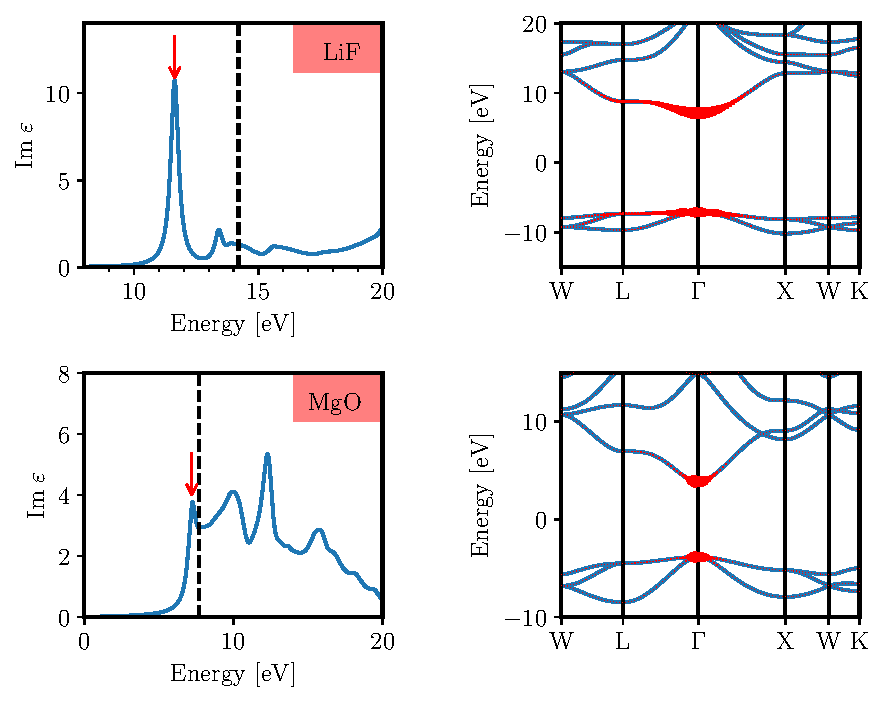
\includegraphics{work/plots/spectra/spectrum_lif_mgo.pdf}
\caption[Optical spectrum and electron-hole coupling coefficients of the first excitation in LiF and MgO.]{Left panels: Imaginary part of the dielectric function of LiF (top) and MgO (bottom).  The fundamental band gaps are marked by  dashed lines and the positions of the lowest-energy excitations by red arrows. Broadenings of 0.2\,eV (LiF) and 0.3\,eV (MgO) are applied. Right panels: Electron-hole coupling coefficients of the  lowest-energy excitation projected onto the band structure. The coupling coefficients are represented as circles, their size is proportional to the magnitude of the coefficients.\label{spectrum_figure}}
\end{figure}
Each electron-hole excitation obtained from the solution of the BSE is expressed as an expansion into independent-particle transitions (Eq.\;\eqref{eh_wf_expansion}). The expansion coefficients are given by the BSE eigenvectors $A^\lambda_{vc\k}$ corresponding to one $v\k\rightarrow c\k$ transition.  For an analysis of excitonic states, it is therefore convenient to introduce the electron-hole coupling coefficients  $w^\lambda_{v\k}$ and $w^\lambda_{c\k}$,  which define the contribution of a given valence or conduction state to the exciton, respectively. In terms of the BSE eigenvectors, they are computed as
%
\begin{equation}
    w^\lambda_{c\k} = \sum_v |A^\lambda_{vc\k}|^2, \qquad w^\lambda_{v\k} = \sum_c |A^\lambda_{vc\k}|^2.
\end{equation}
%
Exemplary, the coupling coefficients projected onto the band structure for the excitonic ground states in LiF and MgO are shown in Figure~\ref{spectrum_figure}, the results for the other materials can be found in Appendix\;\ref{app_excana}.  Additionally, the imaginary part of the dielectric function is shown, where the position of the exciton is marked. In LiF, the first exciton appears at 11.6\,eV and is, therefore, responsible for the large peak in the dielectric function shown in the upper panel. The largest coefficients can be found for transitions from the  valence band maximum (VBM) to the conduction band minimum (CBM) around $\Gamma$, but also transitions in some distance from the BZ center contribute significantly to this exciton. Due to the broad distribution of the coupling coefficients, moderately dense sampled grids (1000-2000 $\k$-points in total) suffice to describe the variation of the excitonic wave function $A^\lambda_{vc\k}$ in reciprocal space and, in turn, to converge the binding energy.\par
Turning to MgO, we find the first excitation at 7.2\,eV. Being a bright excitation, this exciton is responsible for the first peak of the spectrum, which is shown on the left-hand side of the lower panel in Figure~\ref{spectrum_figure}.  As can be seen from the figure, this exciton consists mostly of strongly localized transitions from the VBM to the CBM around $\Gamma$, and other bands contribute only to a much lower extent. Similar observations are made for the other low-binding energy materials GaN, ZnS, and ZnO. This poses a severe problem for computing converged values of the excitonic binding energy as very dense samplings around the center of the BZ are needed to obtain a converged value of the binding energy.\par
%
\begin{figure}[t]
\captionsetup{format=plain}
\centering
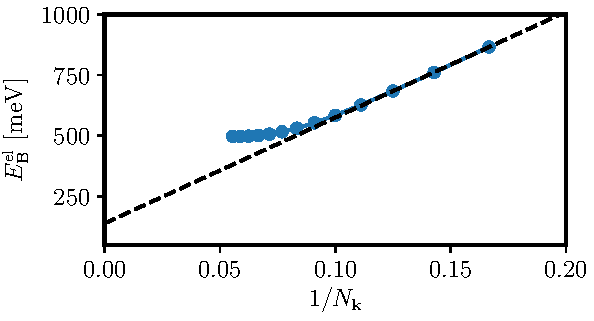
\includegraphics{work/plots/mgo_conv.pdf}
\caption[Excitonic binding energy, $E^\text{el}_\text{B}$, in MgO versus the inverse number of $\k$-points.]{Excitonic binding energy, $E^\text{el}_\text{B}$, of the first exciton in MgO computed with pure electronic screening versus the inverse number of $\k$-points, $N_\k$, in one direction. A~linear extrapolation using the five highest points is shown as dashed line. \label{conv_mgo}}
\end{figure}
%
As an example, Figure~\ref{conv_mgo} shows the excitonic binding energy $E^\text{el}_\text{B}$ in MgO, computed with pure electronic screening on a grid of $N_\k\!\times\!N_\k\!\times\!N_\k$ $\k$-points, versus 1/$N_\k$. It can be seen that the binding energy decreases linearly for coarse grids up to a sampling of 10$\times$10$\times$10 points and only for very dense grids a converging behavior can be observed. When increasing the grid from 17$\times$17$\times$17  to 18$\times$18$\times$18 points, the binding energy changes less than 0.5\%, which is seen as a sufficiently converged value. For the other materials with even lower binding energies, much denser grids would be necessary to reach convergence. However, such dense samplings  are computationally not affordable  with equally distributed $\k$-points, so that there were other methods developed like hybrid meshes. In the case of GaN, for instance, it was shown that the excitonic ground state can be converged by a dense sampling of an inner part of the BZ, which would otherwise require 2 million points distributed equally over the whole Brillouin zone\cite{draxl_gan}. Unfortunately, such a technique is not implemented in the current version of \exciting{}. Therefore, it is not possible to obtain properly converged values for the binding energies such that a different approach is needed to enable quantitative predictions within this thesis. It is presented in Section~\ref{subsec_compapproach}.\par
A further method used in the literature to overcome the difficulty of dense sampling is a simple extrapolation based on the linear decrease of the binding energy for coarse grids\cite{mgo_wrong_convergence} . However,  we assume that this method does not give the same binding energy as it would be obtained from a truly converged calculation. In MgO, the linear extrapolation, applied using the five highest points, is marked by a dashed line in~Figure~\ref{conv_mgo}. The extrapolation yields a value of around 140\,meV, which is far below the one of the converged system, which is around 500\,meV.
%




%---
\subsubsection{Phonon dispersions, Born effective charges, dielectric tensors}
%-----------------------------
\begin{figure}[t]
\captionsetup{format=plain}
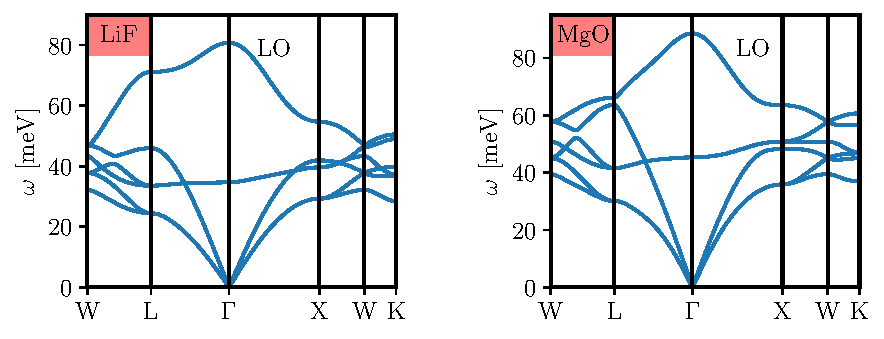
\includegraphics{work/plots/phonons/phonons.pdf}%
\caption[Phonon-dispersion curves for LiF and MgO.]{Phonon-dispersion curves for  LiF (left panel) and MgO (right panel). The longitudinal optical phonon modes most responsible for EPI are marked by~LO. \label{phonon_figure}}
\end{figure}
In Figure~\ref{phonon_figure} the phonon dispersions of LiF and MgO are shown as examples. The results for the other materials can be found in Appendix\;\ref{app_phonon}. As both crystals have a face-centered cubic structure with two atoms in the unit cell, their dispersion relations share some features. Both materials have six phonon modes, three acoustical and three optical. Two of the optical modes are transversal (TO), the other mode is longitudinal (LO), and therefore the most responsible for screening effects from phonons. At $\Gamma$, the two TO modes are degenerate and for both materials, the LO mode has a frequency of around 80\,meV.
\vfill
\newpage
Table~\ref{tab_comp_par}  shows the highest LO frequency $\omega^{\phantom{I}}_\text{LO}$ and the elements of the full static dielectric tensor $\boldsymbol{\varepsilon}_0$ and the Born effective charge tensor $\mathbf{Z}^*$. All materials exhibit large Born effective charges, which results in larger elements of the full dielectric tensors $\boldsymbol{\varepsilon}_0$ compared to the high-frequency tensor $\boldsymbol{\varepsilon}_\infty$ shown in Table~\ref{table_dynscreen}. 
 There is an overall agreement between computed and experimental values (see Table~\ref{tab_exp_data}) with only small discrepancies, in particular with regard to the Born effective charges and the phonon frequencies. A slight deviation of the computed elements of the full static dielectric tensor from the experimental counterparts can be observed, but for all materials the deviation does not exceed 10\%.  Although the dielectric tensor $\boldsymbol{\varepsilon}_0$ does not enter the construction of the screened Coulomb interaction in Eq.~\eqref{w_ph_fourier}, it is instructive to look at this quantity to quantify the effects of EPI on the excitonic binding energy: The tensor on the one hand appears in the limiting case of our first-principles approach in Eq.\;\eqref{w_ph_limit}, and on the other hand is used for evaluations within the Wannier-Mott model through Eq.\;\eqref{eb_rex}.

\begin{table}[t]
\captionsetup{format=plain}
\caption[Computed parameters relevant for EPI.]{Computed parameters relevant for EPI: Elements of the full static dielectric tensor  $\boldsymbol{\varepsilon}_0$, the Born effective charge tensor $\mathbf{Z}^*$, and the highest LO frequency. Only nonvanishing tensor elements are shown.  Parallel and perpendicular ($\parallel,\perp$) are to be understood with respect to the $\mathbf{c}$-axis of the wurtzite crystals.}
\vspace{1mm}
   \begin{tabularx}{\textwidth}{YYYY}
    \hline
    \hline
    Material  & $\boldsymbol{\varepsilon}_0$ & $\omega^{\phantom{I}}_\text{LO}$ [meV] & $|\mathbf{Z}^*|$ [a.u.] \\
    \hline
    LiF  & 9.6  & 83  & 1.1  \\
    MgO  & 10.1 & 91  & 2.0 \\
    ZnS  & 7.8  & 44  & 1.9 \\
    GaN  & 9.0 ($\perp$), 10.0 ($\parallel$)  & 91  & 2.6 ($\perp$), 2.8 ($\parallel$) \\
    ZnO  & 8.5 ($\perp$), 9.3 ($\parallel$)  & 73  & 2.1 ($\perp$), 2.2 ($\parallel$)\\
    \hline
    \hline
    \end{tabularx}
\label{tab_comp_par}
\end{table}

\vfill
\subsubsection{Computational approach for low binding energies}\label{subsec_compapproach}
%-------------------------------------
 \begin{figure}[t]
\captionsetup{format=plain}
\centering
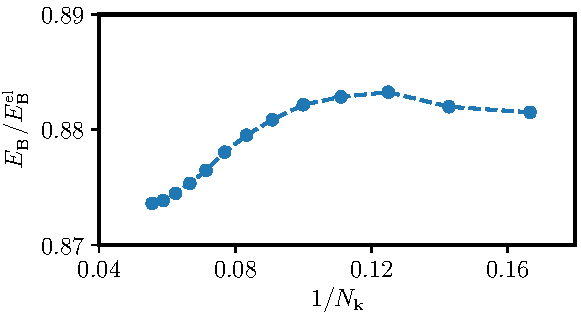
\includegraphics{work/plots/mgo_rel_conv.pdf}
\vspace{-2mm}
\caption[Ratio of the  binding energies $E_\text{B}^{\phantom{l}}$ and $E^\text{el}_\text{B}$ of the first exciton in MgO computed with and without the inclusion of EPI versus the inverse number of $\k$-points.]{Ratio of the  binding energies $E_\text{B}^{\phantom{l}}$ and $E^\text{el}_\text{B}$ of the first exciton in MgO computed with and without the inclusion of EPI  versus the inverse number of $\k$-points $N_\k$ in one direction. \label{conv_rel}}
\end{figure}
With the current implementation of \exciting{}, it is not possible to converge the low excitonic  binding energies in ZnS, GaN, and ZnO due to an insufficient $\k$-point sampling (see discussion in Section~\ref{subsec_exc_ana}). In order to make quantitative predictions within this thesis, we therefore follow an approach based on the use of  results published in the literature. More specifically, we use converged values for the binding energies $E^\text{el}_\text{B}$ and the corresponding excitation energies $E^{\lambda=0}$ obtained from the solution of the BSE using pure electronic screening. These quantities are needed as starting point for the setup of the BSE Hamiltonian in Eq.\;\eqref{h_dir_final} and for an analysis within the Wannier-Mott model in Eq.\;\eqref{eb_rex}. The key idea is that the relative effect of EPI on the binding energy is independent of the $\k$-point sampling if the same starting point is used for every grid. Therefore, also the ratio $E_\text{B}^{\phantom{l}}/E^\text{el}_\text{B}$ between the binding energy using the full screening and the binding energy with pure electronic screening is independent of the sampling. It is thus sufficient to compute both binding energies on a coarse grid and to use this ratio in order to renormalize the converged value for  $E^\text{el}_\text{B}$.\par
To justify the chosen approach, both binding energies are computed for MgO using grids of $N_\k\!\times\!N_\k\!\times\!N_\k$ points and the variation of the ratio  $E_{\text{B}}^{\phantom{l}}/E^\text{el}_{\text{B}}$ versus~$1/N_\k$ is observed. MgO is chosen, as in this material the  binding energy can be studied over a broad range of $1/N_\k$ until it converges. The corresponding values are shown in Figure~\ref{conv_rel}. For all calculations of the phonon BSE term through Eq.\;\eqref{h_dir_final}, the same starting point for the excitation energy $E^{\lambda=0}$ corresponding to a binding energy of $E^\text{el}_\text{B}=498$\,meV is used. The same number of points are used as in Figure~\ref{conv_mgo}, thus the whole range of the linear decrease up to the region where the binding energy converges is covered. As can be seen from the figure, the ratio of the two binding energies varies only very slightly with respect to the $\k$-point sampling and a change from less than 1\%-point can be observed when going from a 6$\times$6$\times$6 grid to a 18$\times$18$\times$18 grid. With increasing density of the grid, the ratio varies less, as for a large number of $\k$-points the two binding energies are converged. Also for the other materials, the ratio of the binding energies varies only very slightly with increasing number of mesh points, and the aforementioned procedure is therefore applied to these materials. The literature values for the binding energy corresponding to the used initial excitation energies can be found in Table~\ref{tab_wm_vs_full} in the next section.\par
 \begin{table}[t]
\captionsetup{format=plain}
\caption[High-frequency dielectric tensor $\boldsymbol{\varepsilon}_\infty$ computed in \exciting{} and in the literature.]{Components of the high-frequency dielectric tensor $\boldsymbol{\varepsilon}_\infty$ as computed in \exciting{} compared to experimental values. For ZnS, GaN, and ZnO, additionally literature values\cite{draxl_gan,zns_bse,zno_bse} are shown, which stem from the publications serving as reference for the binding energy $E^\text{el}_\text{B}$. Parallel and perpendicular ($\parallel,\perp$) are to be understood with respect to the $\mathbf{c}$-axis of the wurtzite crystals. For experimental references see Table~\ref{table_dynscreen}.}
\vspace{1mm}
    \centering
    \begin{tabularx}{\textwidth}{YYYY}
    \hline
    \hline
     Material & \exciting{} & Literature & Experiment \\
     \hline
    LiF & 1.8 & -   & 1.9 \\
    MgO & 2.7 & - & 2.9\\
    ZnS & 4.9 & 5.1  & 5.1 \\
    GaN & 4.8 ($\perp$), 4.9 ($\parallel$) & 5.2 ($\perp$),  5.3 ($\parallel$) & 5.4 ($\perp$), 5.8 ($\parallel$)\\
    ZnO & 3.7 ($\perp$), 3.7 ($\parallel$) & not published  &  3.7 ($\perp$), 3.8 ($\parallel$)\\
    \hline
    \hline
    \end{tabularx}
    \label{tab_highfreq_screen}
\end{table}
It is clear that this procedure does not provide a fully quantitative way to evaluate the effects of EPI since results of different codes using different computational parameters are used. Nevertheless, the BSE implementation within \exciting{} has been shown to be in good agreement with previous works at the same level of theory\cite{Vorwerk_2019} and therefore the findings are seen to be not just of a qualitative nature.\par
This assumption is supported by the values of the high-frequency dielectric tensors  $\boldsymbol{\varepsilon}_\infty$, which agree among the different computations. The components of the dielectric tensors of all investigated materials and their experimental counterparts are shown in Table~\ref{tab_highfreq_screen}. One can observe a slight underestimation of the high-frequency dielectric tensor as computed in \exciting{} compared to the reference values from literature calculations and experiment.  The underestimation  can be attributed to the use of quasiparticle corrections of the electronic structure. Evaluating the screening using the Kohn-Sham band structure, however, a much stronger overestimation is found. Overall, the values are close enough to expect that the published binding energies deviate only slightly from those which would have been obtained with \exciting{} using a dense sampling.
\vfill
%

%-------------------------
%-----------------------------------

%-----------------------------
\subsubsection{Renormalization of the binding energy}
%-------------------------

In Table~\ref{tab_wm_vs_full}, excitonic binding energies  computed with pure electronic screening $E_\text{B}^\text{el}$ and with the additional contribution from EPI $E_\text{B}^{\phantom{l}}$ are presented. The values obtained from our full first-principles approach (BSE) are compared with values obtained from the Wannier-Mott (WM) model and experimental values. The initial excitation energies for the setup of the BSE Hamiltonian (Eq.\;\eqref{h_dir_final}) and the computation within the WM model (Eq.\;\eqref{eb_rex})  are obtained from a BSE calculation employing pure electronic screening. For ZnS, GaN, and ZnO, these values correspond to binding energies  $E^\text{el}_\text{B}$ extracted from the literature\cite{draxl_gan,zns_bse,zno_bse}. The presented values for $E_\text{B}^{\phantom{l}}$ are obtained from one-shot calculations for both the BSE and WM approach, \textit{i.e.}, the binding energies are not updated. The convergence with respect to an update of the binding energy is discussed in Section~\ref{subsec_selfconsistent}.\par
\begin{table}[t]
\captionsetup{format=plain}
 \caption[Binding energies $E_\text{B}^{\phantom{l}}$ as obtained from first-principles calculations, the Wannier-Mott model and experiment.]{Binding energies in meV: $E^\text{el}_\text{B}$ computed with pure electronic screening, and $E_\text{B}^{\phantom{l}}$  with the additional effects of EPI. Results are obtained from our first-principles calculations (BSE) and the Wannier-Mott (WM) model. Experimental (Expt.) values are shown for comparison. Starting values $E^\text{el}_\text{B}$ are extracted from the literature for ZnS\cite{zns_bse}, GaN\cite{draxl_gan}, and ZnO\cite{zno_bse}. For experimental references see Table~\ref{table_dynscreen}. \label{tab_wm_vs_full}}
\vspace{1mm} 
 \centering
 \begin{tabularx}{\textwidth}{YYYYY}
    \hline
    \hline
%  \multicolumn{1}{c}{}& \multicolumn{2}{c}{BSE} & \multicolumn{1}{c}{WM } & \multicolumn{1}{c}{Expt.}\\
%  \hline
 Material & $E^\text{el}_\text{B}$ (BSE) & $E_\text{B}^{\phantom{l}}$ (BSE)  & $E_\text{B}^{\phantom{l}}$ (WM)  &  $E_\text{B}^{\phantom{l}}$ (Expt.) \\
\hline
LiF & 2568   & 2495 &  2502  & 1600\\
MgO & 498    & 435  &  439   & $\,\;85$\,-\,$100$\\
ZnS & 52     & 43   &  42    & $32$\,-\,$36$\\
GaN & 37     & 24   &  21    & $18$\,-\,$28$\\
ZnO & 68     & 48   &  45    & $50$\,-\,$60$\\
    \hline
    \hline
\end{tabularx}  
\end{table}
%
From the values in Table~\ref{tab_wm_vs_full}, we see that the exciton binding energy decreases in all of the investigated materials when EPI is included. However, large differences become apparent with regard to the  magnitude of effects. While a reduction of the binding energy  of around 30\% can be found in GaN and ZnO, there is only a decrease of less than 20\% in MgO and ZnS. In LiF, the binding energy decreases only about~3\%. For these differences, the different lattice polarizabilities, and, in particular,  the dynamics of the screening are responsible. These effects are further discussed in Section~\ref{subsec_dyn_pol_effects}. It can be found that the results obtained from our first-principles approach are close to those obtained within the WM model. For LiF, MgO, and ZnS, only small (relative) deviations can be observed, whereas larger ones are found for GaN and ZnO. As in the two latter materials the effects of EPI are stronger, the deviations between the two approaches become more pronounced. Overall, however, there is a good agreement between the results. When comparing these values, one should be aware of the fact that the ground-state excitons in the investigated materials (except LiF) fulfil the main assumption of the WM model, \textit{i.e.}, they are mostly composed of transitions from the valence band maximum to the conduction band minimum (see Section~\ref{subsec_exc_ana}). Furthermore, only a small number of LO phonon modes is present. Therefore, the assumptions made in Section~\ref{subsec_wm} to solve the WM model  analytically hold such that comparable values can be found as from a  full BSE solution. Our results are further supported by a recently published study\footnote[2]{This study also served as a reference for the converged value of the binding energy $E^\text{el}_\text{B}$ with pure electronic screening.} of the effects of EPI on the excitonic binding energy in ZnS, where a comparable result of 42\,meV was found\cite{zns_bse}.\par 

Moreover, it can be observed that the computed binding energies in ZnS, GaN, and ZnO come much closer to the experimental range when EPI is included, which demonstrates the importance of correctly capturing these effects. In the case of GaN, it should be noted that the literature value of $E^\text{el}_\text{B}=37$\,meV was obtained using a dielectric tensor whose elements are about 10\% smaller than the experimental values (see Table~\ref{tab_highfreq_screen}). An approximate reduction of the binding energy by 8\,meV  ($E^\text{el}_\text{B}=29$\,meV) is reported in the publication when using the experimental values for the high-frequency dielectric tensor\cite{draxl_gan}. Using this value as a starting point, a binding energy of $E_\text{B}^{\phantom{l}}=19$\,meV is obtained. 


For MgO and LiF, the discrepancies between computed and experimental values are still large. However, we do not attribute this observation to an erroneous treatment of EPI but to an overestimation of the binding energy computed with pure electronic screening. Using \exciting{}, binding energies $E^\text{el}_\text{B}$  of 498\,meV (MgO) and 2.568\,eV (LiF) are obtained. Similar large values of 430\,meV and 2.050\,eV are reported in the literature\cite{fuchs_08,low_cost}, where the deviation from our results can be mainly traced back to the fact that we used slightly lower dielectric constants (2.7 compared to~3.0  for MgO and 1.8  compared to around~2.0 for LiF). Within the hydrogen-like WM model, where $E^\text{el}_\text{B}\propto\varepsilon^{-2}_\infty$ (see Eq.\;\eqref{wm_rex}), the effect of larger dielectric constants can be estimated, reducing our values to binding energies of~410\,meV  (MgO) and~2100\,meV (LiF), respectively.  As in the literature\cite{fuchs_08,low_cost} the used values for $\varepsilon_\infty$ are even larger than the experimental ones (1.9 for LiF and 2.9 for MgO), we assume that the binding energies $E^\text{el}_\text{B}$ are overestimating the true values  $E_\text{B}^{\phantom{l}}$ not only by neglecting long-range EPI but also by other effects. It is, however, difficult to specify where this overestimation stems from. One possible reason could be the neglection of the short-range contribution to the electron-phonon coupling in this work. From an evaluation of Eq.\;\eqref{eb_rex}, it can be found that values of around $E^\text{el}_\text{B}=140$\,meV (MgO) and $E^\text{el}_\text{B}=1.7$\,eV (LiF) would correspond to a full binding energy $E_\text{B}^{\phantom{l}}$ within the range of experimental values.\par

\subsubsection{Effects of screening dynamics and lattice polarizability}\label{subsec_dyn_pol_effects}
In the interest of analyzing the effects of  lattice polarizability and dynamical screening  on the excitonic binding energy, we again compare the binding energy computed with pure electronic screening  $E_\text{B}^\text{el}$ with the full binding energy $E_\text{B}^{\phantom{l}}$ including effects from~EPI. As our approach accounts for Fr\"ohlich coupling, one expects that the polarizability of the lattice, \textit{i.e.}, the contribution of the lattice to the dielectric tensor, should determine how strong EPI affects the binding energy. In the derivation of the phonon contribution to the BSE Hamiltonian in Section~\ref{dir_int_ph}, it was further found that the impact of EPI on the binding energy depends on the ability of the lattice to follow the exciton formation. In order to illustrate the dynamical effects, we make use of the WM model. From Eq.\;\eqref{eps_eff}, we recall that in this model the effective dielectric constant screening the exciton formation can be defined by~$E_\text{B}^{\phantom{l}} = E^\text{el}_\text{B}\cdot(\varepsilon_\infty/\varepsilon_\text{eff})^2$. Based on this relation, we introduce the parameter~$f_\text{lat}$~as
%
\begin{equation}\label{flat}
    \varepsilon_\text{eff} = \varepsilon_\infty +f_\text{lat}\cdot(\varepsilon_0 - \varepsilon_\infty), 
\end{equation}
%
which takes values between 0 and 1, and can be interpreted as the fraction of the lattice polarizability contributing to the screening. While a value of 0 indicates that only electrons screen the exciton formation ($\varepsilon_\text{eff}=\varepsilon_\infty$), a value of 1 occurs if the whole lattice polarizability contributes to the screening($\varepsilon_\text{eff}=\varepsilon_0$). All values between 0 and 1 correspond to a fractional contribution of the lattice polarizability. 

\begin{table}[t]
\captionsetup{format=plain}
 \caption[Physical quantities determining the impact of EPI on the excitonic binding energy renormalization.]{Ratio between binding energies $E_\text{B}^{\phantom{l}}/E_\text{B}^\text{el}$ and physical quantities determining the impact of EPI on the binding energy.\label{tab_strength}}
 \vspace{1mm}
 \centering
 \begin{tabularx}{\textwidth}{YYYYY}
    \hline
    \hline
 Material  & $\omega^{\phantom{I}}_\text{LO}/E^\text{el}_\text{B}$& $f_\text{lat}$ [\%] & $\varepsilon_0/\varepsilon_\infty$ & $E_\text{B}^{\phantom{l}}/E_\text{B}^\text{el}$ \\
\hline
LiF    & 0.03 & 0.3 &  5.4   & 0.97 \\
MgO    & 0.2  & 2 &  3.8   & 0.87   \\
ZnS    & 0.8  & 17 &  1.6   & 0.83  \\
GaN    & 2.5  &  25  & 1.9   & 0.65  \\
ZnO    & 1.1  &  14 & 2.4   & 0.70  \\
    \hline
    \hline
\end{tabularx}  
\end{table}
%
In Table~\ref{tab_strength},  the ratios between the highest LO frequency and the binding energy $\omega^{\phantom{I}}_\text{LO}/E_\text{B}^{\text{el}}$,  between the averaged full static dielectric constant and the high-frequency constant $\varepsilon_0/\varepsilon_\infty$, and  between the full binding energy including effects from EPI and the binding energy computed with pure electronic screening $E_\text{B}^{\phantom{l}}/E_\text{B}^\text{el}$ as obtained from BSE are  presented. Additionally, the parameter $f_\text{lat}$ is shown. It can be observed that the larger  $\omega^{\phantom{I}}_\text{LO}$ is compared to  $E_\text{B}^{\text{el}}$, the higher is the lattice contribution $f_\text{lat}$ and, in turn, the smaller is $E_\text{B}^{\phantom{l}}$ compared to $E^\text{el}_\text{B}$. This can be interpreted as follows:~For large binding energies, the exciton formation is so fast that the lattice is unable to form a polarization cloud around the electron-hole pair. The contribution of the lattice polarizability to the screening is very small and the screening stems only from electrons. For small binding energies, in contrast, the exciton formation is slow such that the lattice vibrations have enough time to follow the motion of electron and hole. Consequently, the screening significantly increases when EPI is considered. In LiF, the phonon frequency is much smaller than the binding energy such that  the lattice can follow the fast exciton formation to a very low extent. The binding energy reduces by solely~3\% under the inclusion of EPI as only 0.3\% of the lattice polarizability contribute to the screening.  In the other materials, a larger fraction of the lattice polarizability is able to follow the exciton formation as phonon frequencies and binding energies are closer. In GaN, the phonon frequency is more than 2 times larger than the binding energy, which results in a reduction of the binding energy of 35\%. The  lattice is partly able to follow the slow exciton formation, 25\% of the lattice polarizability contribute to the screening.\par 

Moreover, it can be seen that the reduction from $E^\text{el}_\text{B}$ to  $E_\text{B}^{\phantom{l}}$ indeed depends on the lattice polarizability and, hence, the ratio of the dielectric constants $\varepsilon_0/\varepsilon_\infty$. The larger~$\varepsilon_0$ is compared to $\varepsilon_\infty$, the stronger is the influence of EPI resulting in a larger reduction of the binding energy. Looking at ZnS and ZnO, having comparable ratios $\omega^{\phantom{I}}_\text{LO}/E^\text{el}_\text{B}$ of 0.8 and 1.1 but different ratios $\varepsilon_0/\varepsilon_\infty$ of 1.6 and 2.4, respectively, we see that in ZnO  the binding energy is reduced by 30\%, whereas in ZnS only a reduction of 17\% can be observed. A comparable value is found for MgO due to the large lattice polarizability ($\varepsilon_0/\varepsilon_\infty=3.8$), although in this material the binding energy is 5 times larger than the LO phonon frequency. In LiF, the large lattice polarizability leads to a reduction of the binding energy of 3\%, despite the fact that the phonon frequency is almost negligible compared to the huge binding energy.\par

To demonstrate the importance of correctly treating the screening due to EPI, Table~\ref{tab_eb_dynscreen} shows the binding energy of the various materials computed without and with the inclusion of dynamical effects (the latter are equal to the values shown in Table~\ref{tab_wm_vs_full}). The case of neglecting dynamical effects corresponds to setting the weight in the second and third line of the phonon contribution to the direct BSE term Eq.\;\eqref{h_dir_final} equal to one.
%
\begin{table}[t]
\captionsetup{format=plain}
 \caption[Binding energies computed with and without treatment of  dynamical screening effects.]{Binding energies $E_\text{B}^{\phantom{l}}$ in meV computed with  dynamical (dyn.) and static (stat.) treatment of  screening effects. For comparison, the values calculated with pure electronic screening $E_\text{B}^\text{el}$ and the experimental (Expt.) values are shown as~well. \label{tab_eb_dynscreen}}
 \vspace{1mm}
 \centering
 \begin{tabularx}{\textwidth}{YYYYY}
    \hline
    \hline
 Material  & $E_\text{B}^\text{el}$ &   $E_\text{B}^{\phantom{l}}$ (dyn.) &  $E_\text{B}^{\phantom{l}}$ (stat.) &  $E_\text{B}^{\phantom{l}}$ (Expt.) \\
\hline
LiF & 2568  & 2495  & 1520 & 1600\\
MgO & 498   & 435   & 92  & $\,\;85$\;-\;$100$\\
ZnS & 52    & 43    & 31  & $34$\,-\,$37$\\
GaN & 37    & 24    & 18  & $18$\,-\,$28$\\
ZnO & 68    & 48    & 26  & $50$\,-\,$60$\\ 
    \hline
    \hline
\end{tabularx}  
\end{table}
%
It becomes evident that dynamical effects have a strong influence on the renormalization of the excitonic binding energy. In particular for LiF and MgO, materials with large (computed) binding energies, the neglection of the dynamics leads to binding energies much smaller than the values computed with dynamical screening. This can be explained by the fact that without dynamical effects each mode fully contributes to the screening, whereas in the dynamical case the lattice vibrations follow the exciton formation only to a very low extent in these materials. For LiF and MgO, it can further be observed that the binding energies computed under the assumption of static screening are very close to the experimental values. However, this is only the case due to a strong overestimation of the binding energy $E_\text{B}^\text{el}$ computed with pure electronic screening, as already discussed in the preceding section. For ZnS, GaN, and ZnO, the neglection of dynamical effects similarly leads to a stronger renormalization of the binding energies. At variance with LiF and MgO,  the additional screening effects are smaller, as also in the dynamical case the lattice follows the exciton formation to a large extent as phonon frequencies and binding energies are in the same order of magnitude.\par
Nevertheless, neglecting dynamical effects leads to an underestimation of the binding energies in ZnO and ZnS. In GaN, the computed value moves to the lower limit of the experimental range when a starting value of  $E_\text{B}^\text{el}=37$\,meV is used. However, this value is likely to be overestimated due to an underestimation of the dielectric tensor in the RPA screening (see the discussion in the previous section). Assuming that the correct value is around $E_\text{B}^\text{el}=28$\,meV, a binding energy of $E_\text{B}^{\phantom{l}}=14$\,meV is obtained when dynamical effects of the phonon screening are neglected. Similar to the case of ZnS and ZnO, this value also is below the experimental values, which were found in the range of 18\,-\,28\,meV.\par
In conclusion, the results discussed in this section show that a correct treatment of dynamical effects in the phonon part of the screening is crucial in order not to overestimate the renormalization of the excitonic binding energy due to EPI. It should be stressed  that this is true for materials with large and small binding energies alike, although, for LiF and MgO, the neglection of dynamical effects yields results much closer to experiment which indicates that additional effects might be present. 

\subsubsection{Self-consistent solution of the BSE}\label{subsec_selfconsistent}
%
\begin{figure}[t]
\captionsetup{format=plain}
\centering
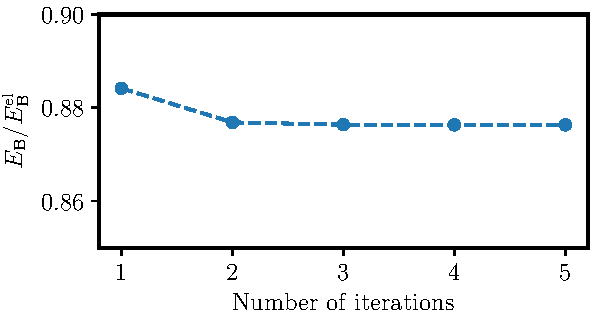
\includegraphics{work/plots/mgo_iteration.pdf}
\caption{Ratio of the binding energies $E_\text{B}^{\phantom{l}}/E^\text{el}_\text{B}$  of the first exciton in MgO versus the number of iterations.\label{iteration_conv}}
\end{figure}
%
As already discussed in Section~\ref{implement_subsec}, the BSE has, in principle, to be solved self-consistently, as the direct term itself depends on the BSE solutions $E^\lambda$.  In Figure~\ref{iteration_conv}, the ratio $E_\text{B}^{\phantom{l}}$ to the initial of value $E^\text{el}_\text{B} = 498$\,meV for the first exciton in MgO is shown versus the number of iterations. The first input energy for the ground-state excitation is the one obtained from pure electronic screening and corresponds to $E^\text{el}_\text{B}$. The resulting binding energy $E_\text{B}^{\phantom{l}}$ after the inclusion of EPI serves as the input energy of the next calculation. From the figure, we can see that sufficient convergence is reached after a few iterations. The reduction between the first to the fourth iteration is roughly 1\% with a change below 0.02\,meV from the third to the fourth iteration. A similar convergence behavior is observed for the other materials. Only one iteration is therefore seen to be satisfactory, as for ZnS, GaN, and ZnO exact numbers are in any case out of reach due to insufficient $\k$-point sampling. Moreover, even for fully converged calculations the error of excitonic binding energies from the solution of the BSE is presumably larger than the changes shown in Figure~\ref{iteration_conv} being  below~1\%.  

\vspace{\fill}
%-------------------------

\newpage
\phantom.
\vspace{3cm}
%----------------------------------
\section{Conclusions and outlook}
%----------------------------------
In the present thesis, a first-principles approach was developed accounting for the influence of electron-phonon interactions (EPI) on excitonic binding energies in polar materials. The derivation includes the coupling to all modes, and no assumptions about the crystal symmetry were made. This represents important progress as previous models are usually based on the coupling to specific modes in isotropic systems. A central element was the derivation of a frequency-dependent phonon contribution to the screened Coulomb interaction, which is completely general and does not require any assumptions about the material. Starting from the Fan-Migdal self-energy of electron-phonon coupling, defining screening effects stemming from phonons on a fundamental level, a real-space expression for the screened Coulomb interaction could be extracted. A leading idea was the expansion in terms of the electron-phonon matrix element, which allows the connection of the developed formalism to the standard notation. The corresponding contribution of phonons to the direct BSE term was derived, which results in an energy-dependent term due to the inclusion of frequency dependence. Being valid for all types of materials, we applied the developed formalism to polar crystals. Here, an explicit expression for the long-range electron-phonon matrix element exists, which is a generalized version of the Fr\"ohlich coupling.  It could be shown that a widely-used screening model is contained as a limiting case in our approach.  The derived expressions for the phonon contribution to screened Coulomb interaction and the direct BSE term were implemented into the all-electron code \exciting{}. \par
With the  developed approach, effects of EPI on the excitonic binding energy of LiF and the prototypical polar semiconductors MgO, GaN, ZnS, and ZnO were investigated. Except LiF, the ground state excitons in these materials have relatively low binding energies in the order of 100\,meV and are rather delocalized in real space. Hence, the excitons are composed of transitions  strongly localized around the center of the Brillouin zone, which requires an extremely dense sampling of this region  in order to converge the binding energy. In the current implementation of \exciting{}, such a sampling technique  is not implemented and converged computations of binding energies are therefore prohibitive for ZnS, GaN, and ZnO. Nevertheless, a computational approach based on the use of converged values published in the literature allowed quantitative predictions also for these materials. Specifically, converged values for the binding energies computed with pure electronic screening were used, and their ratio to the values obtained when including EPI could be computed. Both binding energies computed with \exciting{} and those extracted from the literature overestimate the binding energy if effects from EPI are neglected. After the inclusion of EPI, the computed values come significantly closer to or reach exactly the experimental range for the three materials ZnS, GaN, and ZnO. For LiF and MgO, however, the reduction of the binding energy is not large enough to reach the experimental range. Here, it is assumed that other physical effects, which we do not account for, have an influence on the binding energy as well. However, it is very difficult to specify wh ere the overestimation stems from. One possible reason could be the neglection of the short-range contribution to the electron-phonon coupling in this work. \par 
An analysis within the simplifying Wannier-Mott model yields values very close to those obtained from the first-principles approach. Furthermore, it could be shown that the developed method correctly accounts for dynamical screening effects: In LiF, where the binding energy is above of 2\,eV, EPI reduces the binding energy by less than 1\% as the lattice is unable to follow the fast exciton formation. In the other materials, reductions up to 30\% could be observed. Using results from different codes, the findings are not fully quantitative. However, since the different BSE codes have been shown to produce similar results for other calculations, the deviations are expected to be small.\par
Due to the aforementioned computational difficulties, the effects of EPI on excitonic binding energies were analyzed only for small polar binary compounds, which are already well studied in the literature. We intend to extend the study to more complex polar materials such as $\text{Ga}_2\text{O}_3$ and perovskites, where strong effects of EPI on excitons can be expected.  The implementation of more flexible grids in reciprocal space is urgently needed in this context.  A future goal is also the inclusion of screening effects on the whole optical spectrum, as in the current approach one is limited to study effects on a specific excitation. Furthermore, as temperature effects on excitonic binding energies can be observed in experiments\cite{exciton_perovskites}, it would be interesting to advance the developed formalism in this regard.
%-------------------------
%-------------------------

%-Anhang----------------------------------------------------------\addcontentsline{toc}{section}{Acknowledgements}


\appendix
\phantom{I}
\vspace{3cm}
\section{Supplementary results}
%%
This appendix supplements the results section for the materials not shown in the main text. It provides  phonon dispersions computed and electron-hole coupling coefficients and optical spectra as obtained from the solution of the Bethe-Salpeter equation. 


\subsection{Computational details}\label{app_comp_details}
The numerical results presented in this thesis are obtained with two different codes: The pseudopotential code \textsc{Q\!u\!a\!n\!t\!u\!m} ESPRESSO\cite{quantumespresso} and the full-potential all-electron code \exciting{}\cite{exciting}. In the following, it is summarized which code is used for which calculation, and the computational parameters are presented. The various grids for $\k$ and $\q$-points are given in Table~\ref{grids}. \par

\textsc{Q\!u\!a\!n\!t\!u\!m} ESPRESSO is used for all systems to relax the crystal structure and to calculate the phonon modes as well as the Born effective charges. The ground-state  DFT calculations are performed within the general gradient approximation (GGA) using the PBEsol functional\cite{pbesol}. The LO-TO splitting is computed including the nonanalytical part of the force constants  (see (Eq.\;\eqref{forceconst_an}) through the Born effective charges and the high-frequency dielectric tensor.\par
Ground-state calculations also performed with \exciting{}, followed by the study of excitonic properties  through the solution of the BSE. The basis size is set by the parameter $R_\text{MT}|\mathbf{G+k}|_\text{max} = 7.0$, which is found to be sufficient for converging the ground-state total energy of all systems. For the computation of spectra, the grids are shifted by  ($0.097/N_x$, $0.273/N_y$, $0.493/N_z$) (in lattice coordinates), in order to break the symmetry.  For computing binding energies, however, unshifted grids are used such to include the $\Gamma$-point. This is relevant as, in these materials, the electron-hole coupling coefficients of the lowest-energy excitation are largest at this point. Local-field effects are included up to a cutoff of $|\mathbf{G+q}|_\text{max}=3.0\,\text{a.u.}^{-1}$, and 100 empty states are used in the RPA screening. A scissor operator is used in the screening and the BSE part to adjust the computed band gaps to the experimental values from Table~\ref{table_dynscreen}. In the calculation of optical spectra, four valence bands and five conduction bands are considered, and a broadening of 0.3\,eV is applied. For the computation of the excitonic binding energy, three valence and two conduction bands are included (for LiF, five valence and four conduction bands).\par
%
\begin{table}[t]
\captionsetup{format=plain}
\caption[Grids for $\k$ and $\q$-points employed in the different calculations.]{Grids for $\k$ and $\q$-points employed in the different calculations: Ground state (GS), BSE (for MgO, different grids are used for the calculation of the optical spectrum and the binding energy $E^{\phantom{el}}_\text{B}$), and phonons.\label{grids}}
\vspace{1mm}
   \begin{tabularx}{\textwidth}{YYYY}
    \hline
    \hline
    Material  & $\k$-grid (GS) & $\k$-grid (BSE) & $\q$-grid (phonons) \\
    \hline
    LiF  & 10$\times$10$\times$10 & 12$\times$12$\times$12 & 4$\times$4$\times$4  \\
    MgO   &  10$\times$10$\times$10  & 12$\times$12$\times$12 (spec.) & 4$\times$4$\times$4\\
           &  & 18$\times$18$\times$18 ($E^{\phantom{el}}_\text{B}$) & \\
    ZnS  &  10$\times$10$\times$10  & 12$\times$12$\times$12 & 4$\times$4$\times$4\\
    GaN  &  10$\times$10$\times$8 & 12$\times$12$\times$8 & 4$\times$4$\times$4\\
    ZnO  &  10$\times$10$\times$8 & 12$\times$12$\times$8 & 4$\times$4$\times$4\\
    \hline
    \hline
    \end{tabularx}
\end{table}

\newpage

\subsection{Structure relaxation}
The following Table~\ref{tab_struct} summarizes the relaxed structure constants found for the different materials. 
\begin{table}[h]
\captionsetup{format=plain}
    \caption[Relaxed structure constants of the investigated materials in bohr.]{Relaxed structure constants $a$ in bohr of the investigated materials as computed and found by experiment. For GaN and ZnO in the wurtzite structure, the ratios $c/a$ are shown as well. Experimental values for LiF from\cite{lif_lattice}, for MgO from\cite{mgo_lattice}, for ZnS from\cite{zns_lattice}, for GaN from\cite{gan_lattice}, and for ZnO from\cite{zno_lattice}. }
    \vspace{1mm}
   \begin{tabularx}{\textwidth}{YYYYY}
    \hline
    \hline
     Material & $a$   & $c/a$  & $a$ (Expt.) & $c/a$ (Expt.)\\
     \hline
    LiF &  7.68 & -   & 7.61 & - \\
    MgO &  7.97 & -   &   8.03 & -  \\
    ZnS & 10.12 & -   &    10.22 & - \\
    GaN & 6.02 & 1.63  &   6.03 &  1.63   \\
    ZnO & 6.10 & 1.61 &   6.15 & 1.60   \\
    \hline
    \hline
    \end{tabularx}
    \label{tab_struct}
\end{table} 

\newpage
\subsection{Phonon dispersions}\label{app_phonon}

Figure~\ref{phonon_appendix} shows the computed phonon dispersions of ZnS, GaN, and ZnO along high-symmetry directions in the Brilouin zone.
\begin{figure}[H]
\centering
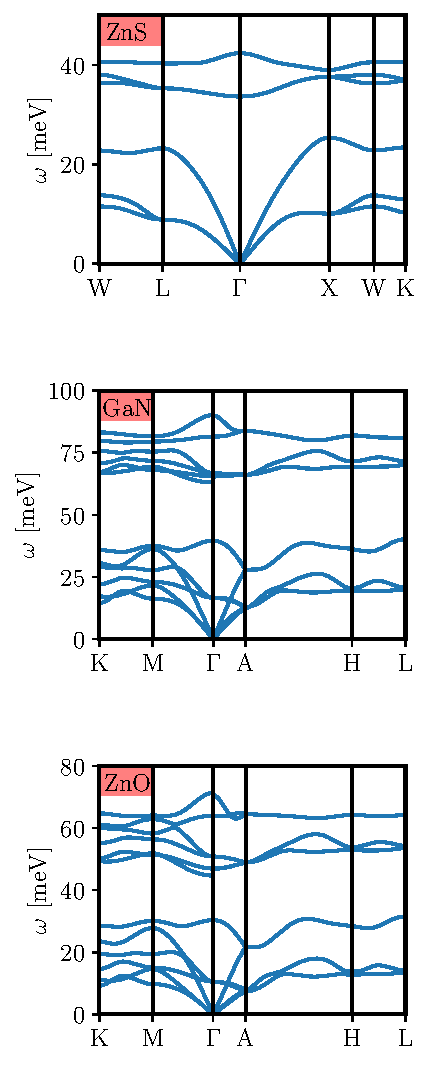
\includegraphics{work/plots/phonons/phonons_app.pdf}

\caption[ Phonon-dispersion curves of ZnS, GaN and ZnO.]{ Phonon-dispersion curves of ZnS (upper panel), GaN (middle panel), and ZnO (lower panel) along high-symmetry directions in the Brillouin zone. \label{phonon_appendix}}

\end{figure}

\subsection{Optical spectra}\label{app_excana}

\begin{figure}[H]

  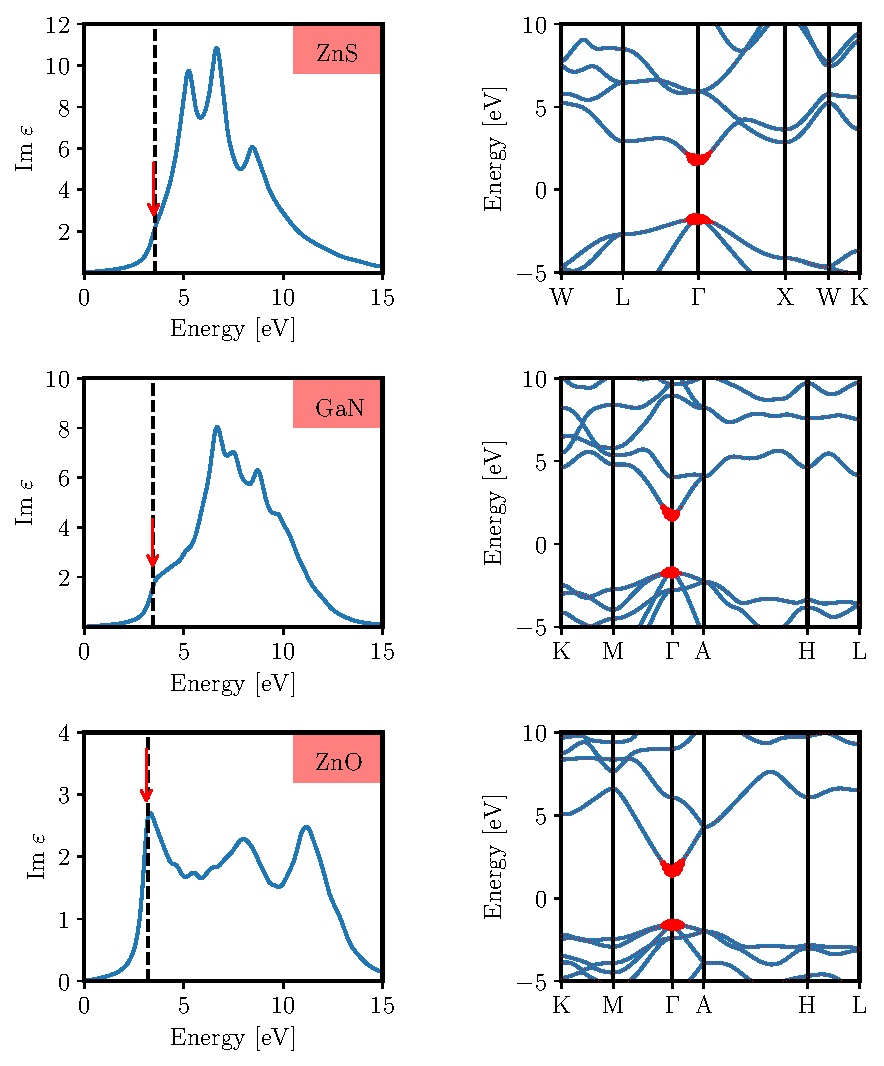
\includegraphics{work/plots/spectra/spectrum_zns_gan_zno.pdf}%
  \caption[Optical spectrum for ZnS, GaN and ZnO.]{Optical spectrum (left) and e-h coupling coefficients of the first exciton (right) of ZnS (upper panel), GaN (middle panel), and ZnO (lower panel). For  GaN and ZnO in the wurtzite structure, the spectra correspond to  light polarized perpendicular to the crystallographic $c$ direction. The position of the first exciton is marked by a red arrow. \label{spectrum_appendix}}
\end{figure}


\newpage
\subsection{Experimental values}

In Table~\ref{tab_exp_data}, we show the experimental values for the elements of the Born-effective charge tensor $\mathbf{Z}^*$, the full static dielectric tensor $\boldsymbol{\varepsilon}_0$, and the highest LO phonon frequencies.

\begin{table}[h]
\captionsetup{format=plain}
\caption[Experimental parameters relevant for EPI.]{Experimental parameters: Elements of the full static dielectric tensor  $\boldsymbol{\varepsilon}_0$ and the Born-effective charge tensor $\mathbf{Z}^*$, and the highest LO frequency in\,meV. Only non-vanishing tensor elements are shown, parallel and perpendicular ($\parallel,\perp$) are to be understood with respect to the $\mathbf{c}$-axis of the wurtzite crystals.  Data for LiF from \cite{lif_charges,lif_tensor,lif_phonon}, for MgO from \cite{mgo_charges,mgo_data}, for ZnS  from \cite{zns_charges,bechstedt2016many}, for ZnO from \cite{zno_data}, and for GaN from \cite{gan_data,gan_charges,gan_tensor}.\label{tab_exp_data}}
\vspace{1mm}
   \begin{tabularx}{\textwidth}{YYYY}
    \hline
    \hline
    Material  & $\boldsymbol{\varepsilon}_0$ & $\omega^{\phantom{I}}_\text{LO}$ [meV] & $|\mathbf{Z}^*|$ [a.u.] \\
    \hline
    LiF  & 9.0 & 82  &  1.0 \\
    MgO  & 9.8 & 89  & 2.0 \\
    ZnS  & 8.3  & 37  & 2.2 \\
    GaN  &  9.5($\perp$), 10.4 ($\parallel$)  & 91  &  2.7($\perp$), 2.8 ($\parallel$) \\
    ZnO  & 7.8($\perp$), 8.9 ($\parallel$)  & 73  & 2.1 ($\perp$), 2.1($\parallel$)\\
    \hline
    \hline
    \end{tabularx}
\end{table}


\newpage

\phantom{.}
\vspace{3cm}
\section{Periodic crystals}\label{bloch_waves}
%------------
%------------
In this appendix, the description of a periodic solid and the properties of Bloch waves in a periodic potential are reviewed. Furthermore, some useful integrals and summations over the crystal lattice are summarized.

%------------
\subsection{Crystal lattice}
%------------

Consider an infinite crystal composed of periodically arranged atoms. The crystal structure is described by a periodically repeated unit cell having the volume $\Omega^{\phantom{I}}_\text{UC}$, which is defined by a set of three basis vectors $\{\mathbf{a}_1,\mathbf{a}_2,\mathbf{a}_3\}$. All integer combination of the basis vectors  define the set of lattice vectors $\{\mathbf{R}\}$. For the theoretical study of crystals, the definition of a reciprocal lattice is useful. The basis vectors $\{\mathbf{b}_1,\mathbf{b}_2,\mathbf{b}_3\}$ in reciprocal space are defined by
%
\begin{equation}
    \mathbf{a}_i\cdot\mathbf{b}_j = 2\pi\,\delta_{ij} \quad   \forall \; i,j \in \{1,2,3\}.
\end{equation}
%
Accordingly, the set of reciprocal lattice vectors  $\{\mathbf{G}\}$ is given by all integer combinations of the reciprocal basis vectors.\par
Usually, just a finite number of unit cells $N_p=N_x\!\times\!N_y\!\times\!N_z$ is considered instead of infinitely large crystals. The set of these unit cells define the Born-von-K\'{a}rm\'{a}n (BvK) volume $V$=$N_p\,\Omega^{\phantom{I}}_\text{UC}$.\newpage
\noindent Commonly used identities over the BvK volume involving the lattice vectors are  given in the following:
%
\begin{align}
    \frac{1}{V}\int_V \text{\!\!d}\mathbf{r}\,e^{i\mathbf{(q-q')\cdot r}} & = \delta_\mathbf{qq'},\\[10pt]
    \frac{1}{N_p}\sum_\mathbf{R}e^{i\mathbf{(q-q')\cdot r}}  & = \delta_\mathbf{qq'}\label{crystalsum}.
\end{align}

%------------
\subsection{Bloch waves}
%------------
In a periodic potential obeying $v(\mathbf{r+R})=v(\mathbf{r})$ for any lattice vector $\mathbf{R}$, Bloch's theorem states that the solutions of the Schr\"odinger equation are of the form 
%
\begin{align}\label{bloch_int}
    \psi_{n\mathbf{k}}(\mathbf{r}) =  u_{n\mathbf{k}}(\mathbf{r})\,e^{i\mathbf{k\cdot r}},
\end{align}
%
where $u_{n\mathbf{k}}(\mathbf{r})=u_{n\mathbf{k}}(\mathbf{r+R})$ has the periodicity of the lattice. Bloch waves are labeled by a band index $n$ and a wave-vector $\mathbf{k}$. Not only electronic wavefunctions, but also other quantites may have a Bloch form, for instance the electron-phonon coupling function can be written as
%
\begin{equation}\label{blochcoupl2}
        g_{\mathbf{q}\nu}(\mathbf{r}) = e^{i\mathbf{q\cdot r}}\,\Delta_\text{P}^{\!\mathbf{q}\nu}v      ^{\phantom{I}}_\text{KS}(\mathbf{r}),
\end{equation}
%
where $\Delta_\text{P}^{\!\mathbf{q}\nu}v      ^{\phantom{I}}_\text{KS}(\mathbf{r})$ is the cell-periodic part of the function. In the main text, the Fourier coefficient of the coupling function is needed which is defined according to Eq.\;\eqref{fourier_coeff1}~as
%
\begin{align}\label{coupling_fourier2}
     \Tilde{g}_{\mathbf{q'}\nu}^{\mathbf{G}}(\mathbf{q}) = \frac{1}{V} \int \text{\!\!d}^3\mathbf{r}\, g_{\mathbf{q'}\nu}(\mathbf{r})\,e^{-i(\mathbf{q}+\mathbf{G})\cdot\mathbf{r}}.
\end{align}
%
Formally, the integration is to be taken over the whole crystal volume $V$, but due to the Bloch-property of the coupling function it can be rewritten as an integral over the unit cell with volume $\Omega^{\phantom{I}}_\text{UC}$. Further, the coefficient is only non-vanishing if $\mathbf{q=q'}$. Considering the Born-von-K\'{a}rm\'{a}n volume, the coordinate of an arbitrary vector $\mathbf{r}$ can \newpage be expressed as the sum of a vector from the unit cell and the coordinate $\mathbf{R}_p$ of the $p$th unit cell. The integral can accordingly be rewritten as
%
\begin{equation}\label{blochdelta}
    \begin{aligned}
    \frac{1}{V} \int_V \text{\!\!d}^3\mathbf{r}\, g_{\mathbf{q'}\nu}(\mathbf{r})\,e^{-i(\mathbf{q}+\mathbf{G})\cdot\mathbf{r}} & =  \frac{1}{V} \int_V \text{\!\!d}^3\mathbf{r}\,\Delta_\text{P}^{\!\mathbf{q}\nu}v      ^{\phantom{I}}_\text{KS}(\mathbf{r})\,e^{-i(\mathbf{q-q'+G)\cdot r}}\\[10pt]
     & = \frac{1}{V} \sum_p\int_{\Omega^{\phantom{I}}_\text{UC}} \text{\!\!d}^3\mathbf{r}\,\Delta_\text{P}^{\!\mathbf{q}\nu}v      ^{\phantom{I}}_\text{KS}(\mathbf{r})\,e^{-i(\mathbf{q-q'+G})\cdot(\mathbf{r}+\mathbf{R}_p)}\\[10pt]
     & = \frac{1}{V} \sum_p e^{-i(\mathbf{q-q'+G})\cdot\mathbf{R}_p}\\[10pt] 
     & \phantom{iiiiiiii} \times \int_{\Omega^{\phantom{I}}_\text{UC}}\text{\!\!d}^3\mathbf{r}\,\Delta_\text{P}^{\!\mathbf{q}\nu}v      ^{\phantom{I}}_\text{KS}(\mathbf{r})\,e^{-i\mathbf{(q-q'+G)\cdot r}}\\[10pt]
     & =  \delta_\mathbf{qq'}\frac{1}{\Omega^{\phantom{I}}_\text{UC}} \int_{\Omega^{\phantom{I}}_\text{UC}} \text{\!\!d}^3\mathbf{r}\, g_{\mathbf{q'}\nu}(\mathbf{r})\,e^{-i(\mathbf{q}+\mathbf{G})\cdot\mathbf{r}}.
    \end{aligned}
\end{equation}
%
In the last equality, the result of the crystal summation in Eq.\;\eqref{crystalsum} was used.


\newpage

\phantom{.}
\vspace{3cm}
\section{Mathematical tools}

\subsection{Fourier transformations}
Here, we summarize the conventions used in the thesis for various Fourier transformations. The expressions are given without proof, they can be found in any book in solid-state theory. 

\subsubsection{Functions in time}\label{fourier_time}

Any function in the time domain $f(t)$ can be transformed into the frequency domain~by
%
\begin{align}
       F(\omega) = \int\text{\!\!d}t\,f(t)\,e^{i\omega t}.
\end{align}                                          
%
The inverse transformation is given by
%
\begin{align}
    f(t) = \frac{1}{2\pi}\int\text{\!\!d}\omega\,F(\omega)\,e^{-i\omega t}.
\end{align}

\newpage

\subsubsection{Functions in real space}
%
Any function in real space $f(\mathbf{r})$   can be represented in terms of its Fourier components $F_\mathbf{G}(\mathbf{q})$ as 
%
\begin{align}\label{fourier_real_onearg}
    f(\mathbf{r}) = \sum^\text{BZ}_\mathbf{q}\sum_\mathbf{G}F_\mathbf{G}(\mathbf{q})\,e^{i\mathbf{(q+G)\cdot r}},
\end{align}
%
where the coefficients of the expansion are given by
%
\begin{align}\label{fourier_coeff1}
    F_\mathbf{G}(\mathbf{q}) = \frac{1}{V}\int_V \text{\!\!d}\mathbf{r}\,f(\mathbf{r})\,e^{-i\mathbf{(q+G)\cdot r}}.
\end{align}
%
The integration extends over the Born-von-K\'{a}rm\'{a}n (BvK) volume $V$. Equivalently, any function depending $f(\mathbf{r,r'})$ on two spatial coordinates can be given by its Fourier representation as
%
\begin{align}
    f(\mathbf{r,r'}) = \frac{1}{V}\sum^\text{BZ}_\mathbf{q,q'}\sum_\mathbf{G,G'}\,e^{i\mathbf{(q+G)\cdot r}}F_\mathbf{G,G'}(\mathbf{q,q'})\,e^{-i\mathbf{(q'+G')\cdot r'}}
\end{align}
%
and the Fourier coefficients are defined as
%
\begin{align}\label{fourier_coeff}
      F_\mathbf{G,G'}(\mathbf{q,q'}) = \frac{1}{V}\int\!\!\int_V \text{\!\!d}\mathbf{r}\text{d}\mathbf{r'}\,e^{-i\mathbf{(q+G)\cdot r}}\,f(\mathbf{r,r'})\,e^{i\mathbf{(q'+G')\cdot r'}}.
\end{align}



%-----------------
\subsubsection{Periodic functions}
%-----------------
In the case of a lattice periodic function  in a periodic crystal depending on one spatial argument, \textit{i.e.} $f(\mathbf{r+R})=f(\mathbf{r})$, only the coefficient corresponding to $\mathbf{q}=0$ will give a contribution to the expansion, such that in this case
%
\begin{align}
    f(\mathbf{r}) = \sum_\mathbf{G}F_\mathbf{G}(0)\,e^{-i\mathbf{G\cdot r}}.
\end{align}
%
Similarly, if a function of two coordinates in real space is periodic with respect to a shift of both arguments by the same lattice vector, \textit{i.e.}, $f(\mathbf{r+R,r'+R})=f(\mathbf{r,r'})$, the Fourier coefficients will only depend on one single reciprocal coordinate and the representation is given by
%
\begin{equation}\label{fourier_periodic}
     f(\mathbf{r,r'}) = \frac{1}{V}\sum^\text{BZ}_\mathbf{q}\sum_\mathbf{GG'}\,e^{i\mathbf{(q+G)\cdot r}}\,F_\mathbf{GG'}(\mathbf{q})\,e^{-i\mathbf{(q+G')\cdot r'}}.
\end{equation}
%
\newpage
\noindent The Fourier coefficients are obtained by integrating over the BvK volume $V$ according~to

%
\begin{align}\label{fourier_coeff_periodic}
      F_\mathbf{GG'}(\mathbf{q}) = \frac{1}{V}\int_V \text{\!\!d}\mathbf{r}\text{d}\mathbf{r'}\,e^{-i\mathbf{(q+G)\cdot r}}\,f(\mathbf{r,r'})\,e^{i\mathbf{(q+G')\cdot r'}}.
\end{align}


\subsection{Residue theorem}\label{residue}
Consider a positively oriented simple closed contour $C$ in the complex plane and a function $f(z)$ of a complex variable $z$ having $n$ poles inside the contour. The residue theorem states that integral over this contour can be evaluated by 
%
\begin{align}
    \int_C \text{\!\!d}z\,f(z) = 2\pi\,i\,\sum_k \underset{z=a_k}{\text{Res}}\,f(z),
\end{align}
%
where $\underset{z=a_k}{\text{Res}}\,f(z)$ is the residue of $f$ with respect to the pole $k$. The residue of a simple pole can be obtained according to
%
\begin{equation}\label{residue_pole}
   \underset{z=a_k}{\text{Res}}\,f(z) = \lim_{z\rightarrow a_k}(z-a_k)\,f(z).
\end{equation}

% A special application of the residue theorem is an integral along the real axis, as shown in Fig.~\ref{residue}. If possible, the contour is in this case chosen such that any additional contribution which is not on the real axis vanishes. In many cases, this is possible as the integrand decays exponentially in the upper or the lower half of the complex plane. Then, only the residues of the poles in the upper or lower half contribute to the integral.


%  \begin{figure}[H]
% \centering
% \begin{tikzpicture}[node distance=8cm]
% \node (xstart) {};
% \node (xend) [right of=xstart] {Re $z$};
% \node (ystart) [below of=xstart, xshift = 4 cm, yshift =  + 5cm] {};
% \node (yend) [above of=ystart,yshift=-2cm] {Im $z$};
% \node (center)[above of=ystart,xshift=3cm,yshift=-5cm] {};



% \node (a1) [above of =xstart, xshift = 2cm,yshift = -8.5cm,  circle,fill,inner sep=1.5pt]{};
% \node (texta1) [above of =xstart, xshift = 2cm,yshift = -9cm]{$a_1$};
% \node (a2) [above of =xstart, xshift = 3cm,yshift = -8.5cm,  circle,fill,inner sep=1.5pt]{};
% \node (texta2) [above of =xstart, xshift = 3cm,yshift = -9cm]{$a_2$};
% \node (a3) [above of =xstart, xshift = 5cm,yshift = -8.5cm,  circle,fill,inner sep=1.5pt]{};
% \node (texta3) [above of =xstart, xshift = 5cm,yshift = -9cm]{$a_n$};

% \node (b1) [above of =xstart, xshift = 3cm,yshift = -7.5cm,  circle,fill,inner sep=1.5pt]{};
% \node (textb1) [above of =xstart, xshift = 3cm,yshift = -7cm]{$b_1$};
% \node (b2) [above of =xstart, xshift = 4.5cm,yshift = -7.5cm,  circle,fill,inner sep=1.5pt]{};
% \node (textb2) [above of =xstart, xshift = 4.5cm,yshift = -7cm]{$b_2$};
% \node (b3) [above of =xstart, xshift = 6.5cm,yshift = -7.5cm,  circle,fill,inner sep=1.5pt]{};
% \node (textb3) [above of =xstart, xshift = 6.5cm,yshift = -7cm]{$b_{m}$};
% \node (textb3) [above of =xstart, xshift = 6.5cm,yshift = -10cm]{$C$};

% \node (dots1) [above of =xstart, xshift = 4.3cm,yshift = -8.5cm]{...};
% \node (dots2) [above of =xstart, xshift = 5.5cm,yshift = -7.5cm]{...};
% \node (linepoint) [above of =xstart, xshift = 5.5cm,yshift = -8cm]{};



% \draw  [->,>=stealth',very thick]   (xstart) -- (linepoint.center) ;
% \draw [line]   (linepoint.center) -- (xend) ;
% \draw [line]   (ystart) -- (yend) ;
% \draw [->,>=stealth',very thick] (center) arc (-10:-170:3cm);
% \end{tikzpicture}

% \caption{\label{residue} An integral along the real axis is expressed as a contour integral.}
% \end{figure}



%------------
%------------





\newpage
%-Literaturverzeichnis--------------------------------------------
\phantomsection
%\nocite{*}
%die Verwendung von bibtex ist Pflicht!!!in
\bibliographystyle{myabbrv}        % modified abbrv with doi
\phantom{.}
\vspace{3cm}
\bibliography{formal/bibliography}
\newpage
\phantom{.}
\vspace{3cm}
\listoffigures
\newpage
\phantom{.}
\vspace{3cm}
\listoftables

%-Glossary-------------------------------------------------------

%\printglossaries
%\glsaddall

%-Kapitel des Anhangs---------------------------------------------

\include{work/appendixA}
\include{work/appendixB}
%usw.

%-Abkuerzungen*---------------------------------------------------

%\include{abbreviations}

%-Danksagung-----------------------------------------------------

%-Danksagung------------------------------------------------------
\phantom.
\vspace{3cm}
\phantomsection\section*{Acknowledgements}
\addcontentsline{toc}{section}{Acknowledgements}
I would first like to thank Prof.\:Dr.\:Dr.\:h.c.\:Claudia Draxl, my academic advisor and first evaluator, for providing the opportunity to conduct my master thesis in her group.\par
 I am grateful to Prof.\:Dr.\:Fabio Caruso for proposing a challenging project and for supervising this thesis. I especially want to thank him for all his support and guidance throughout the time of my work.\par
A special thanks must be given to PD\:Dr.\:Pasquale Pavone. I am thankful for fruitful discussions, for helpful advises, and, in particular, for  extensive and constructive criticism of the manuscript.




%-Lebenslauf------------------------------------------------------

%\include{formal/cv}

%-Selbständigkeiterklärung---------------------------------------
% Ohne Unterschrift
% \phantom.
\vspace{3cm}
\section*{Eigenst\"andigkeitserkl\"arung}

Ich erkläre hiermit, dass ich die vorliegende Arbeit selbstst\"andig verfasst und noch nicht für andere Pr\"ufungen eingereicht habe. S\"amtliche Quellen einschließlich
Internetquellen, die unverändert oder abgewandelt wiedergegeben werden,
insbesondere Quellen für Texte, Grafiken, Tabellen und Bilder, sind als solche
kenntlich gemacht. Mir ist bekannt, dass bei Verstößen gegen diese Grunds\"atze
ein Verfahren wegen T\"auschungsversuchs bzw. T\"auschung eingeleitet wird.\\[10pt]

\noindent Berlin, den
%Mit Unterschrift (Scan)
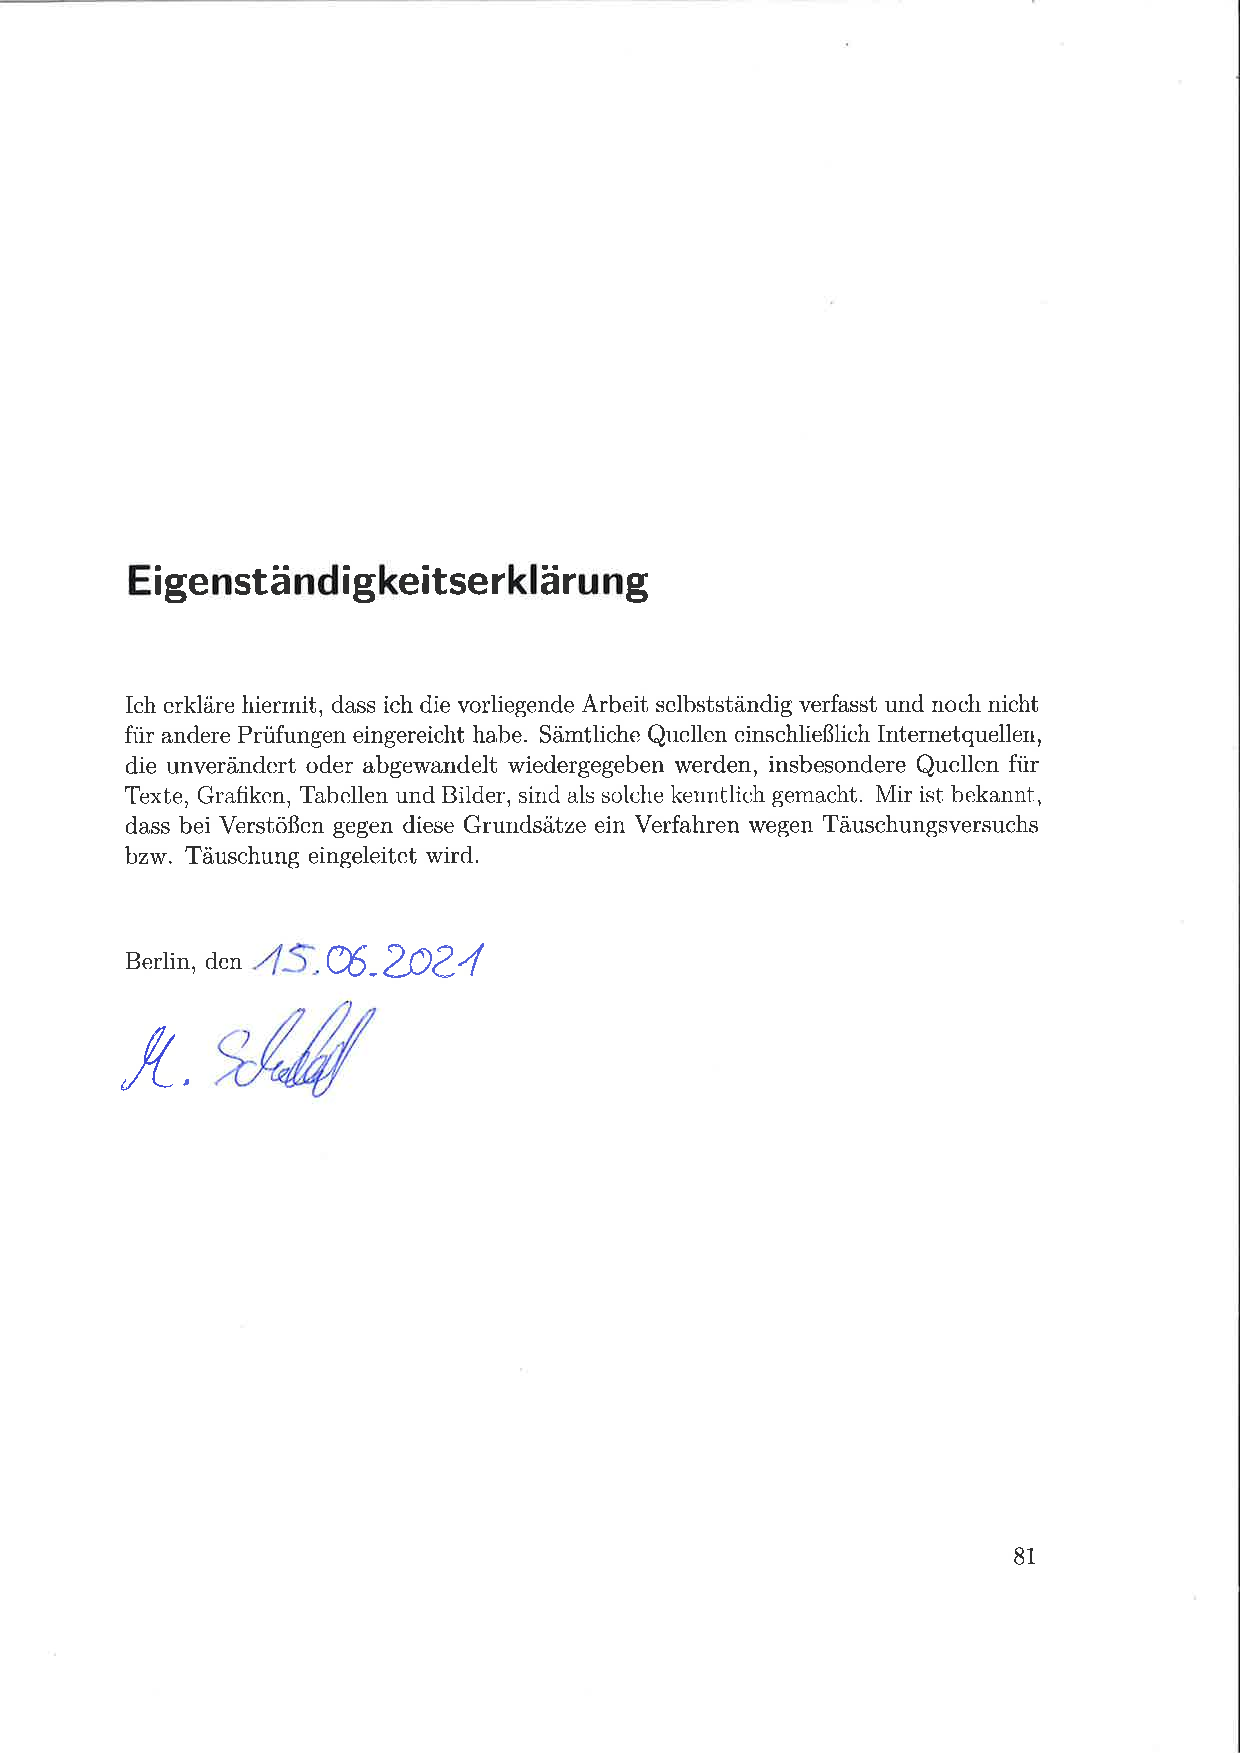
\includepdf[pages={1}]{formal/eigenstaendigkeit}

%-----------------------------------------------------------------

\end{document}